\documentclass{article}

% ICLR 2027 submission (double-blind). Official template files (ICLR/Master-Template, iclr2027, 2026-09-01) are used
% unmodified; no layout parameters are overridden. Main text <= 9 pages; statements, references and appendix are
% outside the limit.
\usepackage{iclr2027_conference,times}
% \iclrfinalcopy  % camera-ready only

%%%%% NEW MATH DEFINITIONS %%%%%

\usepackage{amsmath,amsfonts,bm}

% Mark sections of captions for referring to divisions of figures
\newcommand{\figleft}{{\em (Left)}}
\newcommand{\figcenter}{{\em (Center)}}
\newcommand{\figright}{{\em (Right)}}
\newcommand{\figtop}{{\em (Top)}}
\newcommand{\figbottom}{{\em (Bottom)}}
\newcommand{\captiona}{{\em (a)}}
\newcommand{\captionb}{{\em (b)}}
\newcommand{\captionc}{{\em (c)}}
\newcommand{\captiond}{{\em (d)}}

% Highlight a newly defined term
\newcommand{\newterm}[1]{{\bf #1}}


% Figure reference, lower-case.
\def\figref#1{figure~\ref{#1}}
% Figure reference, capital. For start of sentence
\def\Figref#1{Figure~\ref{#1}}
\def\twofigref#1#2{figures \ref{#1} and \ref{#2}}
\def\quadfigref#1#2#3#4{figures \ref{#1}, \ref{#2}, \ref{#3} and \ref{#4}}
% Section reference, lower-case.
\def\secref#1{section~\ref{#1}}
% Section reference, capital.
\def\Secref#1{Section~\ref{#1}}
% Reference to two sections.
\def\twosecrefs#1#2{sections \ref{#1} and \ref{#2}}
% Reference to three sections.
\def\secrefs#1#2#3{sections \ref{#1}, \ref{#2} and \ref{#3}}
% Reference to an equation, lower-case.
\def\eqref#1{equation~\ref{#1}}
% Reference to an equation, upper case
\def\Eqref#1{Equation~\ref{#1}}
% A raw reference to an equation---avoid using if possible
\def\plaineqref#1{\ref{#1}}
% Reference to a chapter, lower-case.
\def\chapref#1{chapter~\ref{#1}}
% Reference to an equation, upper case.
\def\Chapref#1{Chapter~\ref{#1}}
% Reference to a range of chapters
\def\rangechapref#1#2{chapters\ref{#1}--\ref{#2}}
% Reference to an algorithm, lower-case.
\def\algref#1{algorithm~\ref{#1}}
% Reference to an algorithm, upper case.
\def\Algref#1{Algorithm~\ref{#1}}
\def\twoalgref#1#2{algorithms \ref{#1} and \ref{#2}}
\def\Twoalgref#1#2{Algorithms \ref{#1} and \ref{#2}}
% Reference to a part, lower case
\def\partref#1{part~\ref{#1}}
% Reference to a part, upper case
\def\Partref#1{Part~\ref{#1}}
\def\twopartref#1#2{parts \ref{#1} and \ref{#2}}

\def\ceil#1{\lceil #1 \rceil}
\def\floor#1{\lfloor #1 \rfloor}
\def\1{\bm{1}}
\newcommand{\train}{\mathcal{D}}
\newcommand{\valid}{\mathcal{D_{\mathrm{valid}}}}
\newcommand{\test}{\mathcal{D_{\mathrm{test}}}}

\def\eps{{\epsilon}}


% Random variables
\def\reta{{\textnormal{$\eta$}}}
\def\ra{{\textnormal{a}}}
\def\rb{{\textnormal{b}}}
\def\rc{{\textnormal{c}}}
\def\rd{{\textnormal{d}}}
\def\re{{\textnormal{e}}}
\def\rf{{\textnormal{f}}}
\def\rg{{\textnormal{g}}}
\def\rh{{\textnormal{h}}}
\def\ri{{\textnormal{i}}}
\def\rj{{\textnormal{j}}}
\def\rk{{\textnormal{k}}}
\def\rl{{\textnormal{l}}}
% rm is already a command, just don't name any random variables m
\def\rn{{\textnormal{n}}}
\def\ro{{\textnormal{o}}}
\def\rp{{\textnormal{p}}}
\def\rq{{\textnormal{q}}}
\def\rr{{\textnormal{r}}}
\def\rs{{\textnormal{s}}}
\def\rt{{\textnormal{t}}}
\def\ru{{\textnormal{u}}}
\def\rv{{\textnormal{v}}}
\def\rw{{\textnormal{w}}}
\def\rx{{\textnormal{x}}}
\def\ry{{\textnormal{y}}}
\def\rz{{\textnormal{z}}}

% Random vectors
\def\rvepsilon{{\mathbf{\epsilon}}}
\def\rvtheta{{\mathbf{\theta}}}
\def\rva{{\mathbf{a}}}
\def\rvb{{\mathbf{b}}}
\def\rvc{{\mathbf{c}}}
\def\rvd{{\mathbf{d}}}
\def\rve{{\mathbf{e}}}
\def\rvf{{\mathbf{f}}}
\def\rvg{{\mathbf{g}}}
\def\rvh{{\mathbf{h}}}
\def\rvu{{\mathbf{i}}}
\def\rvj{{\mathbf{j}}}
\def\rvk{{\mathbf{k}}}
\def\rvl{{\mathbf{l}}}
\def\rvm{{\mathbf{m}}}
\def\rvn{{\mathbf{n}}}
\def\rvo{{\mathbf{o}}}
\def\rvp{{\mathbf{p}}}
\def\rvq{{\mathbf{q}}}
\def\rvr{{\mathbf{r}}}
\def\rvs{{\mathbf{s}}}
\def\rvt{{\mathbf{t}}}
\def\rvu{{\mathbf{u}}}
\def\rvv{{\mathbf{v}}}
\def\rvw{{\mathbf{w}}}
\def\rvx{{\mathbf{x}}}
\def\rvy{{\mathbf{y}}}
\def\rvz{{\mathbf{z}}}

% Elements of random vectors
\def\erva{{\textnormal{a}}}
\def\ervb{{\textnormal{b}}}
\def\ervc{{\textnormal{c}}}
\def\ervd{{\textnormal{d}}}
\def\erve{{\textnormal{e}}}
\def\ervf{{\textnormal{f}}}
\def\ervg{{\textnormal{g}}}
\def\ervh{{\textnormal{h}}}
\def\ervi{{\textnormal{i}}}
\def\ervj{{\textnormal{j}}}
\def\ervk{{\textnormal{k}}}
\def\ervl{{\textnormal{l}}}
\def\ervm{{\textnormal{m}}}
\def\ervn{{\textnormal{n}}}
\def\ervo{{\textnormal{o}}}
\def\ervp{{\textnormal{p}}}
\def\ervq{{\textnormal{q}}}
\def\ervr{{\textnormal{r}}}
\def\ervs{{\textnormal{s}}}
\def\ervt{{\textnormal{t}}}
\def\ervu{{\textnormal{u}}}
\def\ervv{{\textnormal{v}}}
\def\ervw{{\textnormal{w}}}
\def\ervx{{\textnormal{x}}}
\def\ervy{{\textnormal{y}}}
\def\ervz{{\textnormal{z}}}

% Random matrices
\def\rmA{{\mathbf{A}}}
\def\rmB{{\mathbf{B}}}
\def\rmC{{\mathbf{C}}}
\def\rmD{{\mathbf{D}}}
\def\rmE{{\mathbf{E}}}
\def\rmF{{\mathbf{F}}}
\def\rmG{{\mathbf{G}}}
\def\rmH{{\mathbf{H}}}
\def\rmI{{\mathbf{I}}}
\def\rmJ{{\mathbf{J}}}
\def\rmK{{\mathbf{K}}}
\def\rmL{{\mathbf{L}}}
\def\rmM{{\mathbf{M}}}
\def\rmN{{\mathbf{N}}}
\def\rmO{{\mathbf{O}}}
\def\rmP{{\mathbf{P}}}
\def\rmQ{{\mathbf{Q}}}
\def\rmR{{\mathbf{R}}}
\def\rmS{{\mathbf{S}}}
\def\rmT{{\mathbf{T}}}
\def\rmU{{\mathbf{U}}}
\def\rmV{{\mathbf{V}}}
\def\rmW{{\mathbf{W}}}
\def\rmX{{\mathbf{X}}}
\def\rmY{{\mathbf{Y}}}
\def\rmZ{{\mathbf{Z}}}

% Elements of random matrices
\def\ermA{{\textnormal{A}}}
\def\ermB{{\textnormal{B}}}
\def\ermC{{\textnormal{C}}}
\def\ermD{{\textnormal{D}}}
\def\ermE{{\textnormal{E}}}
\def\ermF{{\textnormal{F}}}
\def\ermG{{\textnormal{G}}}
\def\ermH{{\textnormal{H}}}
\def\ermI{{\textnormal{I}}}
\def\ermJ{{\textnormal{J}}}
\def\ermK{{\textnormal{K}}}
\def\ermL{{\textnormal{L}}}
\def\ermM{{\textnormal{M}}}
\def\ermN{{\textnormal{N}}}
\def\ermO{{\textnormal{O}}}
\def\ermP{{\textnormal{P}}}
\def\ermQ{{\textnormal{Q}}}
\def\ermR{{\textnormal{R}}}
\def\ermS{{\textnormal{S}}}
\def\ermT{{\textnormal{T}}}
\def\ermU{{\textnormal{U}}}
\def\ermV{{\textnormal{V}}}
\def\ermW{{\textnormal{W}}}
\def\ermX{{\textnormal{X}}}
\def\ermY{{\textnormal{Y}}}
\def\ermZ{{\textnormal{Z}}}

% Vectors
\def\vzero{{\bm{0}}}
\def\vone{{\bm{1}}}
\def\vmu{{\bm{\mu}}}
\def\vtheta{{\bm{\theta}}}
\def\va{{\bm{a}}}
\def\vb{{\bm{b}}}
\def\vc{{\bm{c}}}
\def\vd{{\bm{d}}}
\def\ve{{\bm{e}}}
\def\vf{{\bm{f}}}
\def\vg{{\bm{g}}}
\def\vh{{\bm{h}}}
\def\vi{{\bm{i}}}
\def\vj{{\bm{j}}}
\def\vk{{\bm{k}}}
\def\vl{{\bm{l}}}
\def\vm{{\bm{m}}}
\def\vn{{\bm{n}}}
\def\vo{{\bm{o}}}
\def\vp{{\bm{p}}}
\def\vq{{\bm{q}}}
\def\vr{{\bm{r}}}
\def\vs{{\bm{s}}}
\def\vt{{\bm{t}}}
\def\vu{{\bm{u}}}
\def\vv{{\bm{v}}}
\def\vw{{\bm{w}}}
\def\vx{{\bm{x}}}
\def\vy{{\bm{y}}}
\def\vz{{\bm{z}}}

% Elements of vectors
\def\evalpha{{\alpha}}
\def\evbeta{{\beta}}
\def\evepsilon{{\epsilon}}
\def\evlambda{{\lambda}}
\def\evomega{{\omega}}
\def\evmu{{\mu}}
\def\evpsi{{\psi}}
\def\evsigma{{\sigma}}
\def\evtheta{{\theta}}
\def\eva{{a}}
\def\evb{{b}}
\def\evc{{c}}
\def\evd{{d}}
\def\eve{{e}}
\def\evf{{f}}
\def\evg{{g}}
\def\evh{{h}}
\def\evi{{i}}
\def\evj{{j}}
\def\evk{{k}}
\def\evl{{l}}
\def\evm{{m}}
\def\evn{{n}}
\def\evo{{o}}
\def\evp{{p}}
\def\evq{{q}}
\def\evr{{r}}
\def\evs{{s}}
\def\evt{{t}}
\def\evu{{u}}
\def\evv{{v}}
\def\evw{{w}}
\def\evx{{x}}
\def\evy{{y}}
\def\evz{{z}}

% Matrix
\def\mA{{\bm{A}}}
\def\mB{{\bm{B}}}
\def\mC{{\bm{C}}}
\def\mD{{\bm{D}}}
\def\mE{{\bm{E}}}
\def\mF{{\bm{F}}}
\def\mG{{\bm{G}}}
\def\mH{{\bm{H}}}
\def\mI{{\bm{I}}}
\def\mJ{{\bm{J}}}
\def\mK{{\bm{K}}}
\def\mL{{\bm{L}}}
\def\mM{{\bm{M}}}
\def\mN{{\bm{N}}}
\def\mO{{\bm{O}}}
\def\mP{{\bm{P}}}
\def\mQ{{\bm{Q}}}
\def\mR{{\bm{R}}}
\def\mS{{\bm{S}}}
\def\mT{{\bm{T}}}
\def\mU{{\bm{U}}}
\def\mV{{\bm{V}}}
\def\mW{{\bm{W}}}
\def\mX{{\bm{X}}}
\def\mY{{\bm{Y}}}
\def\mZ{{\bm{Z}}}
\def\mBeta{{\bm{\beta}}}
\def\mPhi{{\bm{\Phi}}}
\def\mLambda{{\bm{\Lambda}}}
\def\mSigma{{\bm{\Sigma}}}

% Tensor
\DeclareMathAlphabet{\mathsfit}{\encodingdefault}{\sfdefault}{m}{sl}
\SetMathAlphabet{\mathsfit}{bold}{\encodingdefault}{\sfdefault}{bx}{n}
\newcommand{\tens}[1]{\bm{\mathsfit{#1}}}
\def\tA{{\tens{A}}}
\def\tB{{\tens{B}}}
\def\tC{{\tens{C}}}
\def\tD{{\tens{D}}}
\def\tE{{\tens{E}}}
\def\tF{{\tens{F}}}
\def\tG{{\tens{G}}}
\def\tH{{\tens{H}}}
\def\tI{{\tens{I}}}
\def\tJ{{\tens{J}}}
\def\tK{{\tens{K}}}
\def\tL{{\tens{L}}}
\def\tM{{\tens{M}}}
\def\tN{{\tens{N}}}
\def\tO{{\tens{O}}}
\def\tP{{\tens{P}}}
\def\tQ{{\tens{Q}}}
\def\tR{{\tens{R}}}
\def\tS{{\tens{S}}}
\def\tT{{\tens{T}}}
\def\tU{{\tens{U}}}
\def\tV{{\tens{V}}}
\def\tW{{\tens{W}}}
\def\tX{{\tens{X}}}
\def\tY{{\tens{Y}}}
\def\tZ{{\tens{Z}}}


% Graph
\def\gA{{\mathcal{A}}}
\def\gB{{\mathcal{B}}}
\def\gC{{\mathcal{C}}}
\def\gD{{\mathcal{D}}}
\def\gE{{\mathcal{E}}}
\def\gF{{\mathcal{F}}}
\def\gG{{\mathcal{G}}}
\def\gH{{\mathcal{H}}}
\def\gI{{\mathcal{I}}}
\def\gJ{{\mathcal{J}}}
\def\gK{{\mathcal{K}}}
\def\gL{{\mathcal{L}}}
\def\gM{{\mathcal{M}}}
\def\gN{{\mathcal{N}}}
\def\gO{{\mathcal{O}}}
\def\gP{{\mathcal{P}}}
\def\gQ{{\mathcal{Q}}}
\def\gR{{\mathcal{R}}}
\def\gS{{\mathcal{S}}}
\def\gT{{\mathcal{T}}}
\def\gU{{\mathcal{U}}}
\def\gV{{\mathcal{V}}}
\def\gW{{\mathcal{W}}}
\def\gX{{\mathcal{X}}}
\def\gY{{\mathcal{Y}}}
\def\gZ{{\mathcal{Z}}}

% Sets
\def\sA{{\mathbb{A}}}
\def\sB{{\mathbb{B}}}
\def\sC{{\mathbb{C}}}
\def\sD{{\mathbb{D}}}
% Don't use a set called E, because this would be the same as our symbol
% for expectation.
\def\sF{{\mathbb{F}}}
\def\sG{{\mathbb{G}}}
\def\sH{{\mathbb{H}}}
\def\sI{{\mathbb{I}}}
\def\sJ{{\mathbb{J}}}
\def\sK{{\mathbb{K}}}
\def\sL{{\mathbb{L}}}
\def\sM{{\mathbb{M}}}
\def\sN{{\mathbb{N}}}
\def\sO{{\mathbb{O}}}
\def\sP{{\mathbb{P}}}
\def\sQ{{\mathbb{Q}}}
\def\sR{{\mathbb{R}}}
\def\sS{{\mathbb{S}}}
\def\sT{{\mathbb{T}}}
\def\sU{{\mathbb{U}}}
\def\sV{{\mathbb{V}}}
\def\sW{{\mathbb{W}}}
\def\sX{{\mathbb{X}}}
\def\sY{{\mathbb{Y}}}
\def\sZ{{\mathbb{Z}}}

% Entries of a matrix
\def\emLambda{{\Lambda}}
\def\emA{{A}}
\def\emB{{B}}
\def\emC{{C}}
\def\emD{{D}}
\def\emE{{E}}
\def\emF{{F}}
\def\emG{{G}}
\def\emH{{H}}
\def\emI{{I}}
\def\emJ{{J}}
\def\emK{{K}}
\def\emL{{L}}
\def\emM{{M}}
\def\emN{{N}}
\def\emO{{O}}
\def\emP{{P}}
\def\emQ{{Q}}
\def\emR{{R}}
\def\emS{{S}}
\def\emT{{T}}
\def\emU{{U}}
\def\emV{{V}}
\def\emW{{W}}
\def\emX{{X}}
\def\emY{{Y}}
\def\emZ{{Z}}
\def\emSigma{{\Sigma}}

% entries of a tensor
% Same font as tensor, without \bm wrapper
\newcommand{\etens}[1]{\mathsfit{#1}}
\def\etLambda{{\etens{\Lambda}}}
\def\etA{{\etens{A}}}
\def\etB{{\etens{B}}}
\def\etC{{\etens{C}}}
\def\etD{{\etens{D}}}
\def\etE{{\etens{E}}}
\def\etF{{\etens{F}}}
\def\etG{{\etens{G}}}
\def\etH{{\etens{H}}}
\def\etI{{\etens{I}}}
\def\etJ{{\etens{J}}}
\def\etK{{\etens{K}}}
\def\etL{{\etens{L}}}
\def\etM{{\etens{M}}}
\def\etN{{\etens{N}}}
\def\etO{{\etens{O}}}
\def\etP{{\etens{P}}}
\def\etQ{{\etens{Q}}}
\def\etR{{\etens{R}}}
\def\etS{{\etens{S}}}
\def\etT{{\etens{T}}}
\def\etU{{\etens{U}}}
\def\etV{{\etens{V}}}
\def\etW{{\etens{W}}}
\def\etX{{\etens{X}}}
\def\etY{{\etens{Y}}}
\def\etZ{{\etens{Z}}}

% The true underlying data generating distribution
\newcommand{\pdata}{p_{\rm{data}}}
% The empirical distribution defined by the training set
\newcommand{\ptrain}{\hat{p}_{\rm{data}}}
\newcommand{\Ptrain}{\hat{P}_{\rm{data}}}
% The model distribution
\newcommand{\pmodel}{p_{\rm{model}}}
\newcommand{\Pmodel}{P_{\rm{model}}}
\newcommand{\ptildemodel}{\tilde{p}_{\rm{model}}}
% Stochastic autoencoder distributions
\newcommand{\pencode}{p_{\rm{encoder}}}
\newcommand{\pdecode}{p_{\rm{decoder}}}
\newcommand{\precons}{p_{\rm{reconstruct}}}

\newcommand{\laplace}{\mathrm{Laplace}} % Laplace distribution

\newcommand{\E}{\mathbb{E}}
\newcommand{\Ls}{\mathcal{L}}
\newcommand{\R}{\mathbb{R}}
\newcommand{\emp}{\tilde{p}}
\newcommand{\lr}{\alpha}
\newcommand{\reg}{\lambda}
\newcommand{\rect}{\mathrm{rectifier}}
\newcommand{\softmax}{\mathrm{softmax}}
\newcommand{\sigmoid}{\sigma}
\newcommand{\softplus}{\zeta}
\newcommand{\KL}{D_{\mathrm{KL}}}
\newcommand{\Var}{\mathrm{Var}}
\newcommand{\standarderror}{\mathrm{SE}}
\newcommand{\Cov}{\mathrm{Cov}}
% Wolfram Mathworld says $L^2$ is for function spaces and $\ell^2$ is for vectors
% But then they seem to use $L^2$ for vectors throughout the site, and so does
% wikipedia.
\newcommand{\normlzero}{L^0}
\newcommand{\normlone}{L^1}
\newcommand{\normltwo}{L^2}
\newcommand{\normlp}{L^p}
\newcommand{\normmax}{L^\infty}

\newcommand{\parents}{Pa} % See usage in notation.tex. Chosen to match Daphne's book.

\DeclareMathOperator*{\argmax}{arg\,max}
\DeclareMathOperator*{\argmin}{arg\,min}

\DeclareMathOperator{\sign}{sign}
\DeclareMathOperator{\Tr}{Tr}
\let\ab\allowbreak

\usepackage[utf8]{inputenc}
\usepackage[T1]{fontenc}
\usepackage{hyperref}
\usepackage{url}
\usepackage{booktabs}
\usepackage{amsmath,amssymb,amsthm}
\usepackage{nicefrac}
\usepackage{microtype}
\usepackage{xcolor}
\usepackage{graphicx}
\usepackage{wrapfig}
\newtheorem{proposition}{Proposition}

% =====================================================================
% NUMBER MACROS — single source of truth. Every value regenerates from the released result files; \pendingnum
% renders a visible red marker so that no placeholder can silently survive into a submitted PDF.
\newcommand{\pendingnum}[1]{\textcolor{red}{\textbf{[#1]}}}
% TRL2D official protocol (The Well), released CNextU-net checkpoint:
\newcommand{\TRLanchorRepro}{0.1934}  % our re-evaluation of the official ckpt
\newcommand{\TRLanchorPub}{0.1956}    % published CNextU-net one-step test VRMSE
\newcommand{\TRLwindows}{873}         % official test windows
\newcommand{\TRLvanilla}{$0.19307 \pm 0.00008$}
\newcommand{\TRLquantum}{$0.19315 \pm 0.00009$}
\newcommand{\TRLmlp}{$0.19314 \pm 0.00019$}
\newcommand{\TDvanilla}{$1.0301 \pm 0.0449$}
\newcommand{\TDquantum}{$\mathbf{0.9528 \pm 0.0542}$}
\newcommand{\TDmlp}{$1.0322 \pm 0.0259$}
\newcommand{\TDnoent}{$1.0156 \pm 0.0433$}
\newcommand{\TDgutz}{$1.0495 \pm 0.1219$}
\newcommand{\MSquantum}{$\mathbf{0.9486 \pm 0.0231}$}
\newcommand{\MSnoent}{$0.9664 \pm 0.0264$}
\newcommand{\MSgutz}{$0.9782 \pm 0.0418$}
\newcommand{\MSanchor}{0.9707}
\newcommand{\MSvanilla}{$0.9867 \pm 0.0196$}
\newcommand{\MSmlp}{$1.0041 \pm 0.0160$}
% Qubit ladder (sprint arena, 2,000 steps, TD k=4, 3 seeds, VRMSE@8):
\newcommand{\QLzero}{$0.9567 \pm 0.2554$}
\newcommand{\QLfive}{$0.8427 \pm 0.0709$}
\newcommand{\QLten}{$0.9332 \pm 0.2166$}
\newcommand{\QLtwenty}{$0.9269 \pm 0.2792$}
\newcommand{\QLthirty}{$0.8447 \pm 0.0511$}
\newcommand{\QLmlp}{$0.9534 \pm 0.1354$}
\newcommand{\QLgeo}{$0.8951 \pm 0.1367$}
\newcommand{\QLgutz}{$0.8393 \pm 0.0463$}
\newcommand{\MechanismVerdict}{interactions appear necessary at the official start; entanglement is not separable
from interaction nonlinearity at three seeds}
% Cross-benchmark matched-control audit (paper/judge/judge.py -> runs/judge/scorecard.md), primary rows:
\newcommand{\AuditQvT}{5\,/\,1\,/\,2}   \newcommand{\AuditQvTp}{0.22}
\newcommand{\AuditQvM}{4\,/\,2\,/\,2}   \newcommand{\AuditQvMp}{0.69}
\newcommand{\AuditMvT}{2\,/\,2\,/\,4}   \newcommand{\AuditMvTp}{1.00}
\newcommand{\AuditREqt}{$+0.04\%$ $[-0.00, +0.08]$}
\newcommand{\AuditREqm}{$+0.53\%$ $[-0.39, +1.45]$}
% Sophelio TEST (single scoring, rule in paper/sophelio/score_test.py):
\newcommand{\SophTEST}{0.9910}
% Allocation study (paper/alloc/analyze.py -> runs/alloc/summary.md; doc 33):
\newcommand{\AllocRows}{TRL2D, rayleigh\_benard, shear\_flow and MHD\_64 with the released CNextU-net, RealPDEBench with its released U-Net and FNO, and the heat plume with the 1HP\_NN U-Net}
\newcommand{\AllocCeilExample}{from 0.039 to 0.34 on shear\_flow and from 0.047 to 0.46 on the heat plume}
\newcommand{\AllocPelzerStatic}{$9.2\%$}
\newcommand{\AllocPelzerPooled}{$1.45\%$}
\newcommand{\AllocPelzerOracle}{$15\%$}
\newcommand{\AllocFNOeff}{93\%}
\newcommand{\AllocPreds}{captured never exceeded $U$; captured rises with $U$ across the 42 row--strategy cells, Spearman $\rho = 0.71$ with row-bootstrap 95\% CI $[0.18, 0.98]$; but routing beats pooling on 5 of 7 rows, failing exactly on the two where no tested corrector captured the error, and gain-predicted routing beats energy routing on only 3 of 7, within noise of learned and proxy routing}
\newcommand{\AllocQvM}{3 rows better, 3 worse, 1 tied; random-effects $+0.006\%$ $[-0.005, +0.017]$}
\newcommand{\AllocPair}{$-0.43\%$ to $+0.01\%$ on the five rows with predictable error, none significant}
\newcommand{\AllocTDC}{13 of 22 (it leads on 9)}
\newcommand{\AllocRange}{0.9--36\%}
% =====================================================================

\title{Utilization over Qubits:\\Rydberg Registers in Physics World Models}

\author{Anonymous}

\makeatletter\def\TableRows#1{\@@input #1 }\makeatother   % generated table rows (expandable inside tabular)
\begin{document}

\maketitle

\begin{abstract}
In hybrid classical--quantum models, how many qubits are available matters less than how well they are used. We attach
an input-dependent Rydberg-atom co-processor, QUOTA, to world models on ten scientific and optimization tasks (fusion,
geothermal, fluid flow and vehicle routing; released checkpoints where available), under decision rules registered before each run, most after earlier test results on the same rows. With the same 30
qubits, routing cuts error by up to 36\%, against 7\% for the standard design that averages features before the qubits
see them; a linear corrector on the same routes, writing spatial modes that averaging cannot reach, already gets 29 of
the 36 points, input-adaptive routing adds 3--4 points, and a similarly sized classical core behind the same routing design gains as much (at 100 qubits, ten 10-atom
groups, on shear flow the register beat a smaller graph-blind MLP, 199 against 244 parameters, on five new seeds by
2.5\%, but a registered follow-up did not establish that edge against a graph-aware GNN of similar size or a wider MLP). With the backbone fixed (the rest retrained),
error falls as the budget grows to 100 qubits, by 16\% on shear flow and 8\% on convection, and levels off at 200 although
the captured share still rises; registered bounds for 50, 100 and 200 qubits (oracle-coverage diagnostics from test
labels, not forecasts) held on every seed. The gains come from allocating by signal type: a router trained on residuals
predicts, from the input and the backbone's forecast, which frequency modes (Fourier octaves and wavelet tiles) to
correct; selected modes get a classical bypass plus the register, the rest a classical head. Atom positions, detunings and tethers between atom groups are also set per input, but in a registered control
the tested geometry and tethers did not pass the rule for a gain. At the sizes we can simulate, we detect no consistent quantum
superiority over matched classical cores. A descriptive closed form, $G(K)=\eta\,U_\infty[1-(1+K/K_0)^{1-a}]$ with
$a\approx2$, tracks the share of error energy removed by $K$ qubits, where $U_\infty$ is the output basis's reachable share (for
any core) and $\eta$ a core's fill.
\end{abstract}

\section{Introduction}
\label{sec:intro}

Learned physics simulators are now central to scientific machine learning, from turbulence and magnetohydrodynamics
\citep{ohana2024thewell,mccabe2025walrus} to tokamak plasmas \citep{boschi2026tokamind,rousseau2026tokamark} and
real-world flow measurements \citep{hu2026realpdebench}. In parallel, a fast-growing literature inserts small
quantum circuits into such models: hybrid neural operators \citep{ma2025qufex,liu2026hqfnet,ali2026phqfno},
quantum adapters for frozen networks \citep{koikeakino2025quantumpeft,liu2025qpa,raj2025quic}, and quantum-informed
priors for turbulence \citep{wang2026qiml,xue2026qcml}. Whether the quantum part does what a classical
module with the same interface and parameter count could not is rarely tested; where tested, apparent
edges vanish under equal-tuning classical baselines \citep{bowles2024better,pandey2026qrcbaselines}.

We run that test at scale, on the analog neutral-atom model family that current hardware natively evolves
\citep{kornjaca2024aquila}. QUOTA (\emph{Qubit Utilization thrOugh Trained Allocation}) is a Rydberg register (one atom is one qubit)
whose allocation is learned, not hand-placed. Per-atom detunings are functions of each input; geometry and drives are
trained by gradient; register size and graph are chosen by architecture search; band-limited or routed insertions
decide which modes (or, per input, which error tiles) the atoms serve. It is inserted into the \emph{released}
checkpoints of published models and compared with a parameter-matched MLP core behind the identical interface, a
no-interaction ablation, and a mean-field control, under kill rules fixed before each run. The premise is a division of labor:
a pretrained classical model handles the easily digitized part of a field, and a small qubit budget is worth only as
much as it is utilized on the part each input gets wrong. We separate two claims. Utilization, not qubit count, governs the gain. Whether a
quantum core exploits a given utilization better than a classical one is a second claim; at the sizes we can simulate we detect no consistent quantum superiority, and we claim no equivalence margin.

\begin{figure}[t]
\centering
\IfFileExists{fig_arch.pdf}{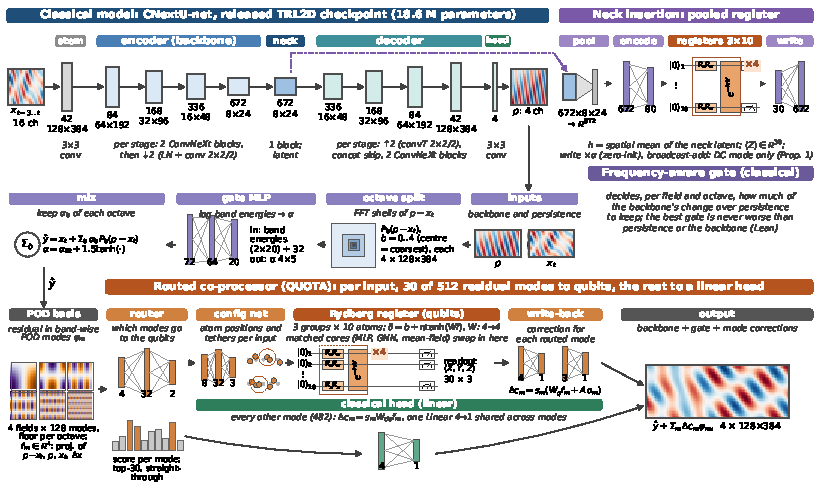
\includegraphics[width=0.97\linewidth]{fig_arch.pdf}}{}
\caption{Architecture with tensor sizes (TRL2D). Each module has a coloured band (its name) and a line on its role.
Top: the released CNextU-net (slabs: channels, height$\times$width) and the standard pooled register in its neck
(Prop.~\ref{prop:pool}). Middle: the frequency-aware gate. Bottom: the routed co-processor, with the register at
gate level; matched classical cores swap into its slot. Bars: fully connected layers. Other backbones:
Appendix~\ref{app:arch}.}
\label{fig:overview}
\end{figure}

\paragraph{Contributions.}
\begin{enumerate}
  \item \textbf{Input-dependent allocation of qubits} (\S\ref{sec:system}, \S\ref{sec:alloc}, Fig.~\ref{fig:overview}):
  each prediction's error is split into Fourier octaves and band-wise POD modes; a router picks input-dependent modes,
  mostly coarse, for a classical bypass plus 30 Rydberg atoms whose positions, detunings and tethers are set per input,
  the rest to a classical head, behind a frequency-aware gate between backbone and persistence. With the same 30 atoms error falls by
  \AllocRange{} across rows, 36\% on convection against 7\% pooled; a linear corrector writing non-DC modes gives 29 of the
  36 points, adaptive routing 3--4, and matched classical cores gain as much.
  \item \textbf{Hybrid scaling with the qubit budget} (\S\ref{sec:alloc}, Appendix~\ref{app:hscale}): with the classical
  model fixed, error falls from 0 to 100 qubits, by 16\% on shear flow and 8\% on convection, and levels off at 200,
  tracked by a descriptive closed form; bounds for 50, 100 and 200 qubits, registered before the runs, held on all 18 seeds.
  \item \textbf{Proofs of where qubits can help} (\S\ref{sec:why}, Lean 4): a register fed spatially averaged (\emph{pooled}) features, the standard design, reads and writes only the DC mode of the latent it is attached to (Proposition~\ref{prop:pool}); routed corrections are
  bounded per Fourier band; the optimal band gate is never worse than persistence or the backbone.
  \item \textbf{A matched-control audit on released models} (\S\ref{sec:audit}): eight physical benchmarks (turbulence,
  MHD, convection, shear flow, tokamak transport and equilibrium, geothermal flow), real-world flows (RealPDEBench) and vehicle routing with two released solvers
  (Appendix~\ref{app:routing}), with similarly sized classical cores (MLP, GNN on its own learned graph, mean-field
  register) in the register's slot; a long-horizon TRL2D edge (\S\ref{sec:trl2d}) did not replicate on a registered fourth seed.
\end{enumerate}

\section{Related work}
\label{sec:related}

\paragraph{Quantum modules in classical surrogates.} Hybrid FNO and U-Net variants
\citep{ma2025qufex,liu2026hqfnet,ali2026phqfno} and quantum-informed turbulence priors \citep{wang2026qiml,xue2026qcml}
typically report gains without parameter-matched cores or released-checkpoint anchors; the closest in-model study, a 5-qubit
mixer in a 3-D FNO, beat a larger dense mixer but not its matched MLP-mixer \citep{papierz2026hqlpfno}. Quantum
adapters for frozen language models \citep{koikeakino2025quantumpeft,liu2025qpa} use quantum circuits to
\emph{generate} classical weights, so inference is classical by construction; our inference-inertness finding
reaches the same deployment regime empirically, the classical-surrogate regime of \citet{schreiber2023surrogates}. Reservoir and attribution studies show that apparent quantum edges
shrink under equal-tuning classical baselines \citep{pandey2026qrcbaselines,pandey2026qrcdimension} and reach nulls
with matched controls and multiplicity correction \citep{chen2026qeat,gillani2026audit,levy2026sidecar,herbort2026cloud};
the register-free QSWM finds a short-horizon edge on cellular automata \citep{sun2026qswm}. We follow the benchmarking
cautions of \citet{bowles2024better} and \citet{schuld2022advantage}, adding pre-registration, kill rules, and
released-checkpoint anchors across eight domains.

\paragraph{Analog ansätze, dequantization, and scaling.} Rydberg reservoirs \citep{bravo2022rydbergqrc,kornjaca2024aquila}
and quantum neural operators \citep{wang2025quanonet} report gains against quantum or unmatched baselines. ReCon co-trains atom positions and drives derivative-free
\citep{silver2024recon}, ResQ feeds inputs into detunings on fixed lattices \citep{chen2026resq}, and PulserDiff
differentiates pulses and positions \citep{pulserdiff2025}; position gradients were argued ineffective under the divergent $r^{-6}$
term \citep{dekeijzer2025consensus}, which we bound by clamping distances while training geometry by exact statevector
autodiff. Variational models that are both trainable and non-dequantizable exist, but on specially constructed learning
problems \citep{gilfuster2025dequant}, and trained quantum models admit classical shadows
\citep{keller2026shadow}; our dequantization suite measures this on a trained world model. Saturation in qubit count
has been reported in non-parameter-matched sweeps \citep{ionq2026scaling,vyskubov2026scaling,zabihi2026hqpinn} and is
predicted by a frozen-block bound \citep{qi2026lego}; our ladder adds a 0-qubit arm and a matched core.

\paragraph{Spectral limits of neural surrogates.} Neural networks fit low frequencies first
\citep{rahaman2019spectral}, and neural PDE solvers lose long rollouts through high-frequency error
\citep{lippe2023pderefiner}. We give the mirror-image statement for insertion modules: a pooled module reads and
writes only the DC mode, whatever its core (Proposition~\ref{prop:pool}).

\section{QUOTA: the register, its insertion, and the controls}
\label{sec:system}

\paragraph{Insertion.} A backbone produces a latent field $z \in \mathbb{R}^{d \times N}$ over $N$ spatial positions.
The standard insertion pools $h = \frac1N\sum_{s} z_{:,s}$, applies a core $c(h) \in \mathbb{R}^{m}$, and writes back a
zero-initialized gated broadcast $z_{:,s} \leftarrow z_{:,s} + \alpha \odot U c(h)$ for every $s$ ($\alpha = 0$ at
initialization, so the inserted model starts exactly at the released checkpoint). Six audit rows insert at a
field-valued latent (a U-Net or operator neck); two (the Sophelio starter model and TokaMind) insert at a vector
latent, where the core sees the whole latent and no pooling occurs. \S\ref{sec:move} replaces this insertion by
band-limited and routed ones.

\paragraph{Register core.} Each 10-atom register evolves under
$H/\hbar = \sum_i \tfrac{\Omega_\ell}{2} X_i - \sum_i \delta_{\ell,i} n_i + \sum_{i<j} C_6 |r_i - r_j|^{-6} n_i n_j$
with input-conditioned detunings $\delta_{\ell,i} = b_{\ell,i} + \pi\tanh(W_\ell h)_i$ ($W$ zero-initialized in the pooled
neck, Gaussian with s.d.\ 0.1 in the routed co-processor),
trainable drives $\Omega_\ell$, times $\tau_\ell$ and 2-D atom coordinates $r_i$ (distances clamped at $0.5\,R_b$),
$L{=}4$ layers of a first-order split (per-atom $R_z(\delta)R_x(\Omega)$, then the diagonal interaction phase), and
$\langle Z_i\rangle$ readout (the routed co-processor also reads $\langle X_i\rangle,\langle Y_i\rangle$). Thirty atoms are three blockade-decoupled registers, keeping trainability fixed across
the qubit ladder \citep{cerezo2025barren}. Training uses an exact complex64 statevector propagator with autograd,
cross-checked against CUDA-Q ($\max_i|\Delta\langle Z_i\rangle| \le 10^{-6}$, 12 qubits).

\paragraph{Controls.} Every control implements the identical pool$\to$core$\to$residual interface at matched total
parameters (the MLP core's width is set from the register's allocated parameter count; at the TRL2D neck the cores
differ by 124 parameters, 0.08\% of the core and under 0.001\% of the 18.6-million-parameter model). \emph{Matched MLP:} a one-hidden-layer MLP core. \emph{No-interaction:} $V_{ij}\equiv 0$ from step 0 (a product state; removes
entanglement and the interaction nonlinearity). \emph{Mean-field (Gutzwiller):} the interaction phase replaced by its
Hartree decoupling $\theta_i = \tau\sum_{j\ne i} V_{ij}\langle n_j\rangle$, which keeps the $V_{ij}(r)$ nonlinearity and
trainable geometry but forbids entanglement. The ladder removes structure, then interactions, then entanglement alone.

\paragraph{Cost and deployment.} Every experiment, from fine-tuning the released backbones to exact register simulation, ran on a single NVIDIA DGX Spark (one GB10 chip, 128\,GB unified memory). Exact simulation is the price: one TRL2D fine-tuning step (released CNextU-net, forward, backward and AdamW, batch 4) takes 504\,ms for the backbone, 511\,ms ($+1.4\%$) with the MLP core,
and 595\,ms ($+18\%$) with the 30-atom register. Trained neck registers are inference-inert, so deploying them needs no quantum hardware (Appendix~\ref{app:dynamic}).

\paragraph{Probabilistic variant.} Following functional generative networks \citep{alet2025fgn}, a noise draw $\xi_m$
enters the configuration network, so each draw gives the input its own atom positions, detunings and tethers and one
ensemble member $\hat y_m$. Training minimizes the fair energy score \citep{gneiting2007scoring},
$\mathrm{ES}=\frac1M\sum_m\|\hat y_m-y\|-\frac{1}{M(M-1)}\sum_{m<m'}\|\hat y_m-\hat y_{m'}\|$ ($M{=}2$, norms in VRMSE
units, i.e.\ divided by each window's own target variance, which makes it observation-weighted and not strictly
proper), and a validation-tuned scale $\tau$ sets the spread (Appendix~\ref{app:fgn}).

\section{Protocol}
\label{sec:protocol}

\paragraph{Hypothesis and kill rule.} H1: the register improves the benchmark metric over a parameter-matched
classical core trained with identical hyperparameters and step budget; if the core is statistically indistinguishable
or better across seeds, H1 is rejected for that regime (rule fixed before each round). Each benchmark has one primary
row fixed a priori. Tuning (Optuna, train/validation only) gives every model, backbone included, the same trial
budget; TEST is scored once.

\paragraph{Statistics.} Per row, seed-paired relative gains, paired $t$ tests and the paired 95\% CI half-width;
across rows, a tie-aware sign test and a random-effects pool (Table~\ref{tab:auditfull}); on TRL2D, per-trajectory
Wilcoxon tests, Holm-corrected. $\pm$ is the standard deviation over three seeds.

\paragraph{Pre-registration.} Hypotheses, kill rules and decision rules were timestamped before the corresponding
runs (self-attested for review; code, logs and the record are released); the one extension registered after its
models' results were known (\S\ref{sec:trl2d}) is labelled as such. Each final configuration saw TEST once, but some
later protocols were designed after earlier TEST results on the same rows; Appendix~\ref{app:claims} labels every claim
confirmatory or exploratory accordingly.

\section{Results}
\label{sec:results}

\subsection{The register ties a matched classical core across eight benchmarks}
\label{sec:audit}

\begin{table}[t]
\centering
\caption{From the published state of the art to classical $+$ qubits (test split; lower is better except $S$; three
seeds unless noted). Published: PDE-FM (shear flow, convection), Flowers 4$\to$1 (TRL2D), EddyFormer (MHD), CNextU-net (rollout), released U-Net (RealPDEBench), RouteFinder, RADAR (RRNCO), CaliciBoost (Caco-2; $^\P$not re-derivable from training data, App.~\ref{app:caco2}); $^\#$+test-time search). Our best: strongest classical result (Appendix~\ref{app:sota}; $^e$ensemble), bold if below published; other bold: best register-comparison arm; vs columns at 30 qubits (seeds better in parentheses). Top: routed co-processor on a fixed fine-tuned CNextU-net; persistence 0.0646, 0.2024, 0.5761, 0.418; convection on every test window. Middle: pooled register in each neck ($^\dagger$two length-matched seeds; $^\ddagger$backbone tuned under an earlier objective). Bottom: register in the model's own latent (rollout four seeds, RouteFinder and Caco-2 five; $^\S$bf16). Full statistics: Table~\ref{tab:auditfull}.}
\label{tab:audit}
\footnotesize
\setlength{\tabcolsep}{2.5pt}
\resizebox{\linewidth}{!}{%
\begin{tabular}{lccccccccc}
\toprule
Benchmark & Published & Our best & Our classical & $+$MLP & $+$30 qubits & $+$50 & $+$100 & vs MLP & vs classical \\
\midrule
\multicolumn{10}{l}{\emph{Routed co-processor: input-dependent qubit configuration}} \\
\TableRows{tab_routed_rows.tex}
\midrule
\multicolumn{10}{l}{\emph{Standard design: pooled register in the neck}} \\
FNO arena (TRL2D data) & --- & --- & 0.9567 & 0.9534 & \textbf{0.8447} & --- & --- & $+11.4\%$ (3/3) & $+11.7\%$ (2/3) \\
MHD (MHD\_64)$^\dagger$ & 0.1160 & \textbf{0.1154}$^e$ & 0.1897 & 0.1897 & \textbf{0.1896} & --- & --- & $+0.0\%$ (2/2) & $+0.0\%$ (2/2) \\
convection (RB) & 0.0415 & \textbf{0.0403}$^e$ & 0.4563 & 0.5275 & \textbf{0.4221} & --- & --- & $+20.0\%$ (3/3) & $+7.5\%$ (1/3) \\
shear flow & 0.0345 & \textbf{0.0198} & 0.2686 & \textbf{0.2539} & 0.2659 & --- & --- & $-4.7\%$ (2/3) & $+1.0\%$ (2/3) \\
tokamak transport (TORAX) & --- & --- & 0.0158 & \textbf{0.0141} & 0.0168 & --- & --- & $-19.2\%$ (0/3) & $-6.4\%$ (2/3) \\
geothermal plume (1HP)$^\ddagger$ & --- & --- & 0.0291 & 0.0292 & \textbf{0.0288} & --- & --- & $+1.3\%$ (2/3) & $+1.2\%$ (2/3) \\
fusion equilibrium ($S\uparrow$)$^\ddagger$ & 0.9959 & 0.9949 & 0.7905 & 0.7848 & \textbf{0.7929} & --- & --- & $+1.0\%$ (2/3) & $+0.3\%$ (1/3) \\
tokamak signals (TokaMark) & 0.140 & \textbf{0.1334}$^e$ & 0.1509 & 0.1504 & \textbf{0.1501} & --- & --- & $+0.2\%$ (1/3) & $+0.5\%$ (2/3) \\
\midrule
\multicolumn{8}{l}{Neck rows better\,/\,worse\,/\,tied (sign test)} & \AuditQvM{} ($p{=}\AuditQvMp$) & \AuditQvT{} ($p{=}\AuditQvTp$) \\
\midrule
turbulence, rollout 13:30 (TRL2D) & 1.01 & \textbf{0.9892} & 0.9892 & 1.0101 & \textbf{0.9660} & --- & --- & $+4.4\%$ (2/4) & $+2.3\%$ (1/4) \\
real flow, foil (RealPDEBench) & 0.00948 & \textbf{0.00931} & 0.00948 & \textbf{0.00939} & \textbf{0.00939} & --- & --- & $0.0\%$ & $+1.0\%$ \\
routing, RouteFinder (gap \%)$^\S$ & 8.58 & \textbf{6.02}$^\#$ & 8.65 & --- & \textbf{8.61} & --- & --- & --- & $+0.5\%$ (2/5) \\
routing, RRNCO ACVRP (gap \%) & 2.61 & \textbf{2.41}$^\#$ & \textbf{3.49} & --- & 3.71 & --- & --- & --- & $-6.2\%$ (0/3) \\
molecules, Caco-2 (TDC, MAE) & 0.256$^\P$ & 0.276 & 0.362 & \textbf{0.345} & 0.437 & --- & --- & $-26.6\%$ & $-20.7\%$ \\
\bottomrule
\end{tabular}}
\end{table}
\begin{figure}[t]
\centering
\IfFileExists{fig_outputs_all.pdf}{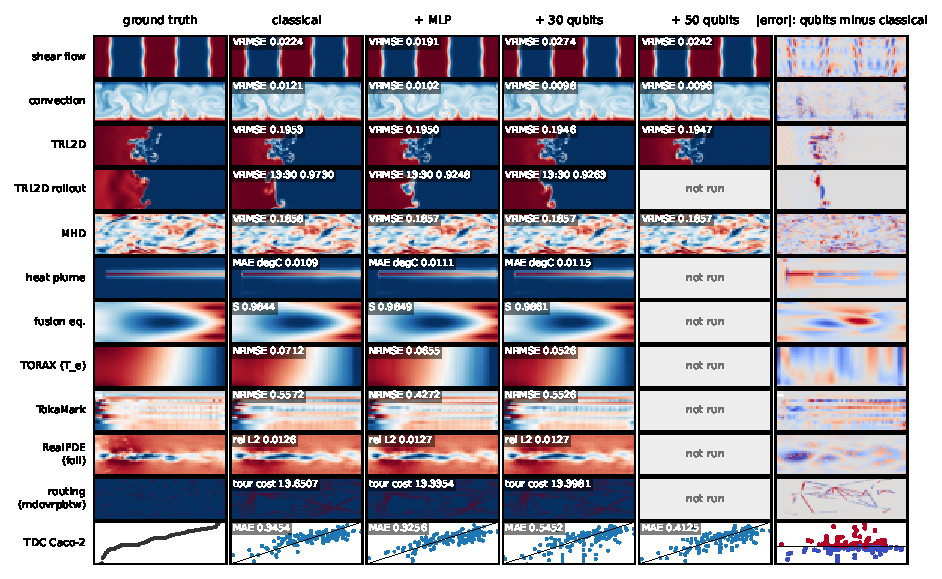
\includegraphics[width=\linewidth]{fig_outputs_all.pdf}}{}
\caption{Model outputs against ground truth, one sample each, fixed in advance, on every benchmark with register arms
(not RRNCO). Columns: classical, $+$ matched MLP, $+$30 and $+$50 qubits (routed co-processor of Table~\ref{tab:audit}, top,
on shear flow, convection, TRL2D and MHD; TRL2D rollout: step 22 of 30; the pooled neck register elsewhere; ``not run'': no 50-qubit model), and the change in absolute error from classical to
the largest register shown (blue: lower). Panels carry that sample's error ($S$ for fusion: higher is better). TDC
Caco-2: predicted against true permeability; routing: tours. Notes per row: Figure~\ref{fig:outputs_all}.}
\label{fig:fields_well}
\end{figure}


Table~\ref{tab:audit} reads left to right: published state of the art, our classical model, and the same model with a
matched MLP or with qubits. The rows use the released checkpoints of The Well's CNextU-net \citep{ohana2024thewell} and
of TokaMind \citep{boschi2026tokamind} on TokaMark \citep{rousseau2026tokamark}, the official U-Net pipelines of a
groundwater heat-transport surrogate \citep{pelzer2025heat} and of the Fusion Equilibrium Challenge
\citep{waller2026fusion}, a TORAX benchmark \citep{citrin2024torax}, and our FNO arena. Against the best published numbers (PDE-FM \citep{soares2025pdefm}, PhysiX \citep{nguyen2025physix}, Flowers \citep{muser2026flowers}, EddyFormer \citep{du2025eddyformer}), our shear-flow hybrid is lower (0.0207 vs 0.0345, full test); a gated three-backbone ensemble is numerically close on convection (0.0403 vs 0.0415; best single model 0.0425) and 1\% lower on TRL2D (0.1909 vs 0.1930, same 4$\to$1 protocol), with more compute; on MHD a retrained Flowers backbone with a metric-aligned fine-tune is 1.0\% above as one model (0.1172 vs 0.1160) and at parity as a two-backbone ensemble (0.1154); TokaMark is matched by one Scratch run (0.1379 vs 0.140) and 4.7\% lower with a post hoc three-run ensemble (0.1334). The margins come from the classical part, a frequency gate with persistence; the routed co-processor adds 12--13\% on shear flow and 5--6\% on convection, where the error is predictable (Figure~\ref{fig:fields_well}), and matched classical cores match it. In
the neck no comparison is significant after correction (sign test $p=\AuditQvMp$ against the matched core;
Figure~\ref{fig:audit}). Separately, a pooled register reads and writes only the spatial mean of its latent (Proposition~\ref{prop:pool}); we do not test whether this explains the null.
Where a fine-tuned model beats a published number, the backbone alone beats it within seed noise, so those gains
belong to fine-tuning (Appendix~\ref{app:sota}); four neck rows are imprecise (paired 95\% CI half-widths 53--99\%,
Appendix~\ref{app:audit}).

\subsection{A candidate effect that did not replicate: long-horizon rollouts on TRL2D}
\label{sec:trl2d}

On TRL2D we fine-tuned the official CNextU-net in two registered rounds. With a one-step objective every model
improves on the checkpoint indistinguishably (backbone \TRLvanilla, MLP \TRLmlp, register \TRLquantum). Trained through
rollouts \citep{brandstetter2022message} and scored on The Well's long-horizon window 13:30 (published 1.01), the
register was the only model below the checkpoint on three seeds (\TDquantum{} vs \TDvanilla{} and MLP \TDmlp), but a
registered fourth seed did not replicate the edge (Table~\ref{tab:trl2d}, Appendix~\ref{app:perseed}).









\subsection{What pooling constrains: the insertion's DC latent mode}
\label{sec:why}

\begin{proposition}[a pooled register sees only the spatial mean of its latent]\label{prop:pool}
Let $P(z) = \frac1N\sum_{s=1}^{N} z_s$ be mean pooling over $N$ positions and let $g$ satisfy $\sum_s g_s = 0$.
Then $P(z+g) = P(z)$; in particular $P$ is invariant to adding any multiple of a non-DC discrete Fourier mode
($\zeta^N = 1$, $\zeta \ne 1$). A spatially constant write-back $c$ is orthogonal to every zero-mean field,
$\sum_s c\, g_s = 0$. Hence the insertion of \S\ref{sec:system} reads and writes only its latent's DC spatial mode, whatever its core. In any orthonormal basis, a perfect correction of the
coefficients in a set $T$ leaves exactly the energy outside $T$.
\end{proposition}

{\sloppy All four statements are proved in Lean~4 with Mathlib \citep{demoura2021lean4,mathlib2020}, standard axioms only (Appendix~\ref{app:lean}).\par} Call the share of the error energy in the modes
an insertion can read and write its \emph{utilization ceiling}. The proposition concerns the insertion latent; a
downstream decoder could spread a DC latent change over spatial outputs, so for pooled insertions we report the
\emph{measured} DC share of the output error, not a proved ceiling. On TRL2D
(Table~\ref{tab:bands}, Appendix~\ref{app:spectral}) the DC shell holds \textbf{2.9\%} of the fine-tuned model's one-step error energy; the backbone
misses 8--11\% of the one-step change at $1\le|k|\le 4$ but 34--45\% at $|k|\ge 17$, the spectral bias of neural
surrogates \citep{rahaman2019spectral,lippe2023pderefiner}. Paired over seeds, the register's only measurable effect is
at $k{=}0$ ($-0.49\% \pm 0.21$ of that band's error, 3/3 seeds; matched MLP $+0.10\% \pm 0.19$); every other band
moves within noise. The classical core is confined to the same mode, which is why the two tie.

\subsection{Raising utilization: aiming the insertion where the error lives}
\label{sec:move}

\begin{table}[t]
\centering
\caption{Correcting only the low-frequency or high-order part of a model's prediction (test split unless noted;
three seeds). RealPDEBench airfoil: relative $L_2$ on 5{,}140 test windows; the corrector acts on the
lowest $3{\times}4{\times}4$ space--time Fourier modes of the prediction. Fusion equilibrium (Sophelio):
score $S$ on validation; the corrector writes PCA components $k\ge8$ of a frozen model.}
\label{tab:move}
\small
\setlength{\tabcolsep}{4pt}
\begin{tabular}{lcccc}
\toprule
Model (benchmark) & Model alone & $+$linear & $+$MLP & $+$qubits \\
\midrule
U-Net, released (RealPDEBench) $\downarrow$ & 0.00948 & \textbf{0.00937} & 0.00939 & 0.00939 \\
FNO, released (RealPDEBench) $\downarrow$ & 0.01413 & 0.01292 & \textbf{0.01267} & \textbf{0.01267} \\
frozen NAS model (Sophelio, validation) $\uparrow$ & 0.9864 & --- & 0.9876 & 0.9879 \\
\bottomrule
\end{tabular}
\end{table}

If pooling is capped by the DC share, an insertion aimed where the error lives should help, and help any core
(Table~\ref{tab:move}). On the RealPDEBench airfoil \citep{hu2026realpdebench}, a low-mode corrector lowers the
released U-Net's test relative $L_2$ from 0.00948 to 0.00937 and the FNO's by 10\%; a linear map captures most of it,
and the register equals its matched MLP to four digits. On the Fusion Equilibrium Challenge (full-data pipeline), a
coupling that writes only the fine PCA components lifts VALID $S$ by $+0.0012$ to $+0.0015$ with either core; the
register leads its matched MLP by $+0.0002$ ($p \ge 0.41$), or by $+0.0010$ ($p=0.09$ corrected) with a
register-selected learning rate (Appendix~\ref{app:move}).

\paragraph{Evaluation error, persistence, and a frequency-aware gate.} On rayleigh\_benard and shear\_flow, persistence
beats The Well's published baselines and every backbone we fine-tuned, though not the foundation models PDE-FM (both rows) and PhysiX (convection) (Fig.~\ref{fig:gate}a): the benchmark's per-window VRMSE is dominated by
low-variance windows that MSE-trained backbones barely weight. A causal gate between backbone and persistence per Fourier
octave (its optimum is proved never worse than either) cuts shear\_flow's test VRMSE from 0.2297 to 0.0272. Routing then sends the
reachable error to the qubits (Fig.~\ref{fig:gate}b), and the register, a GNN on the same graph and an MLP all reach
about 0.020 (Appendix~\ref{app:gate}). Trained end to end with the metric as loss, a three-backbone gated ensemble reaches 0.0403 on
rayleigh\_benard (full test; persistence 0.2024).

\begin{figure}[t]
\centering
\IfFileExists{fig_gate.pdf}{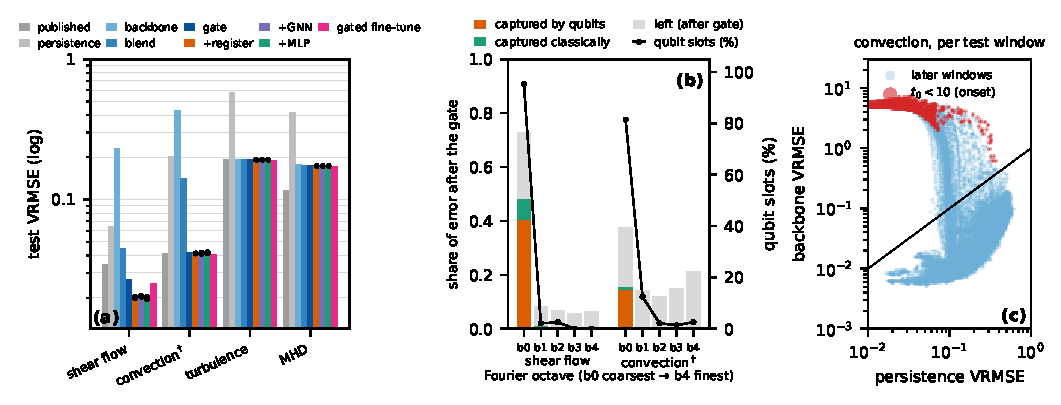
\includegraphics[width=\linewidth]{fig_gate.pdf}}{}
\caption{Where the error sits on the four Well benchmarks (shear flow, Rayleigh--B\'enard convection, turbulent
radiative layer, 3-D MHD). (a) Test VRMSE, log scale, from the published best model through persistence
($\hat y_{t+1}{=}x_t$), our backbone, the frequency gate, and the gate plus qubits, GNN or MLP (dots: seeds;
$^\dagger$stratified test sample). (b) After the gate, the share of the remaining error in each Fourier octave captured
by the qubits, by the classical head, or left; the line gives the router's share of the 30 qubits per octave: 80--95\%
go to the coarse octave that holds the predictable error. (c) Convection, per test window: at convection onset (red)
the backbone is 10--100$\times$ worse than persistence; the gate corrects it.}
\label{fig:gate}
\end{figure}

\subsection{Which input-dependent allocation? A registered cross-benchmark study}
\label{sec:alloc}

\begin{figure}[t]
\centering
\IfFileExists{fig_alloc.pdf}{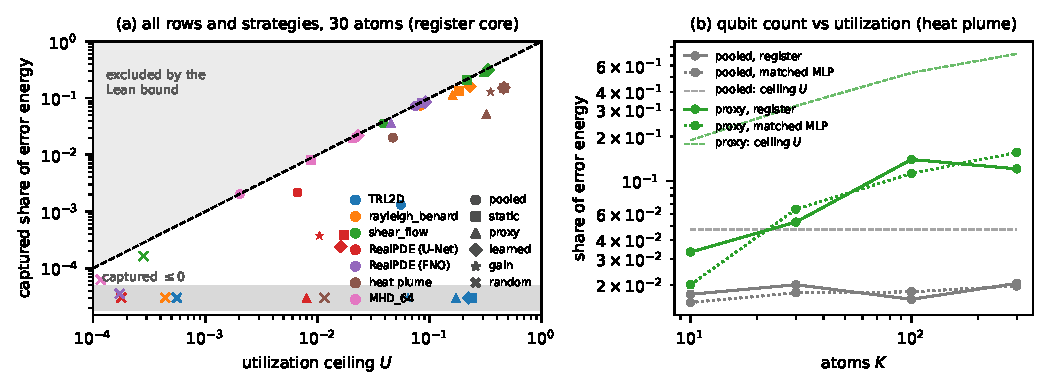
\includegraphics[width=\linewidth]{fig_alloc.pdf}}{\fbox{\parbox{0.9\linewidth}{\centering\pendingnum{fig\_alloc.pdf missing}}}}
\caption{Allocation study (frozen backbones, test split, three seeds). (a) Captured share of each backbone's error energy
against the utilization ceiling $U$ of the allocation, for every row and strategy with the register core; no point can lie above the diagonal. (b) On the heat plume, adding atoms to the pooled insertion
changes nothing (its ceiling is the DC share); routed atoms keep improving as their ceiling grows. Cores coincide throughout (dotted: matched MLP).}
\label{fig:alloc}
\end{figure}

\begin{table}[t]
\centering
\caption{Allocation study, 30 atoms, register core, test split, mean of three seeds. Pooled: the audit's insertion
(ceiling = DC share). Best: the register's validation-best tile strategy, its utilization ceiling $U$, the captured
share of error energy and the test-metric gain over the frozen backbone (VRMSE; relative $L_2$ on RealPDEBench); the last
column is the register's seed-paired gain over its matched MLP at that strategy. On TRL2D and RealPDEBench (U-Net) every
tile strategy captures at most 0.0004, and the listed one is the tie-broken validation choice. rayleigh\_benard's mean
gain is tail-driven: the convection onset (4\% of windows) gives 47\%; median VRMSE $-0.3$ to $-0.5\%$. $^\dagger$Released checkpoint does not
reproduce its published number under our evaluator (Appendix~\ref{app:sota}).}
\label{tab:alloc}
\footnotesize
\setlength{\tabcolsep}{3pt}
\begin{tabular}{lccccccc}
\toprule
 & \multicolumn{2}{c}{pooled} & \multicolumn{4}{c}{best tile strategy} & \\
\cmidrule(lr){2-3}\cmidrule(lr){4-7}
Row (frozen backbone) & DC share & gain & strategy & $U$ & captured & gain & reg.\ vs MLP \\
\midrule
%ALLOC-ROWS-BEGIN
TRL2D (CNextU-net) & 0.056 & $+0.06\%$ & static & 0.238 & 0.000 & $+0.00\%$ & $+0.00\%$ (0/3) \\
rayleigh\_benard (CNextU-net) & 0.083 & $+6.69\%$ & proxy & 0.161 & 0.113 & $+36.25\%$ & $-0.48\%$ (1/3) \\
shear\_flow (CNextU-net)$^\dagger$ & 0.039 & $+6.77\%$ & learned & 0.335 & 0.316 & $+26.29\%$ & $+0.03\%$ (3/3) \\
MHD\_64 (CNextU-net)$^\dagger$ & 0.002 & $+0.11\%$ & gain & 0.023 & 0.022 & $+0.87\%$ & $+0.00\%$ (1/3) \\
RealPDEBench (U-Net) & 0.007 & $+0.12\%$ & static & 0.017 & 0.000 & $+0.01\%$ & $-0.00\%$ (0/3) \\
RealPDEBench (FNO) & 0.074 & $+3.32\%$ & gain & 0.091 & 0.085 & $+3.87\%$ & $+0.01\%$ (3/3) \\
Heat plume (1HP\_NN U-Net) & 0.047 & $+1.45\%$ & static & 0.459 & 0.152 & $+9.23\%$ & $-0.18\%$ (1/3) \\
%ALLOC-ROWS-END
\bottomrule
\end{tabular}
\end{table}

\paragraph{Design.} To separate \emph{where} the atoms work from \emph{what} computes there, we freeze each backbone and
train a co-processor to correct its residual $r = y - p$ in an orthonormal multi-level Haar basis ($r$ is the training target; at inference the co-processor sees only causal inputs and $p$). Per input, a strategy picks
the $K$ tiles the atoms read and write: \emph{pooled} (the audit's insertion), \emph{static}, \emph{proxy},
\emph{learned}, \emph{gain} (the budgeted optimum) or \emph{random}
(Appendix~\ref{app:alloc}). Atoms sit at their tiles, so the allocation sets the interaction graph, and every core
starts as the same linear corrector. Proved bounds fix what can be measured: the captured share never exceeds the \emph{utilization ceiling} $U$, ceilings nest, and a broadcast correction removes at most the DC energy. Rows: \AllocRows; $K=30$, three
seeds, every choice on validation, test once; the protocol and its two amendments were registered before the runs.

\paragraph{Allocation sets the ceiling; predictability sets how much of it is reached.} With the same 30 atoms,
routing raises the ceiling far above the pooled DC share (Table~\ref{tab:alloc}; e.g.\ \AllocCeilExample), and where
the backbone's error is systematic the gain follows: routed atoms cut mean VRMSE by 36\% on rayleigh\_benard and 26\% on
shear\_flow against about 7\% pooled (both relative to released backbones that persistence beats in the mean,
Appendix~\ref{app:gate}; a linear corrector alone: 29\% and 26\%, so the cores add 7.5 points and none); on the heat plume 30 static atoms lower error by \AllocPelzerStatic{} against
\AllocPelzerPooled{} pooled (oracle \AllocPelzerOracle), and the matched MLP does as well; RealPDEBench's FNO reaches \AllocFNOeff{} of $U$. On TRL2D
nothing is captured by any strategy or core, even under oracle placement with a 44\% ceiling. Yet with the residual
supplied as a feature the same pipeline captures 99.7\% of it, so the released turbulence backbone's fine-scale error is
not predictable by these correctors from causal inputs. The registered predictions split accordingly (\AllocPreds).

\begin{figure}[t]
\centering
\IfFileExists{fig_hybrid_scaling.pdf}{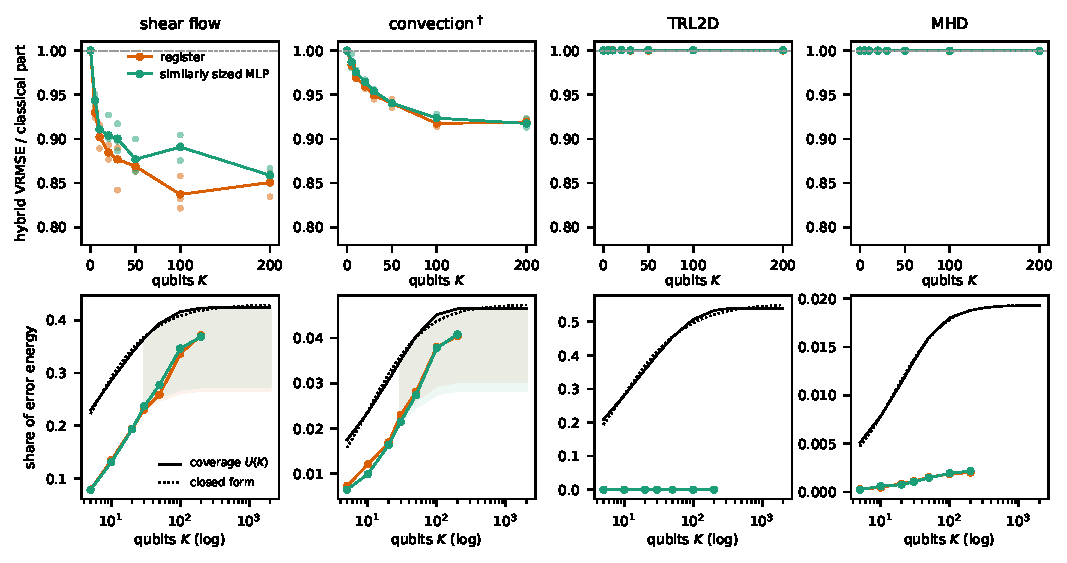
\includegraphics[width=0.78\linewidth]{fig_hybrid_scaling.pdf}}{}
\caption{Hybrid scaling with the qubit budget, backbone fixed, rest retrained per budget (three seeds; dots are seeds; $K$ counts atoms in
groups of at most 10, so the largest joint quantum state has 10 atoms). Top: test VRMSE
relative to the classical part ($K{=}0$). Error falls with each added atom group up to 100 qubits on shear flow and convection
($^\dagger$stratified test sample), where the correctors capture the backbone's error, and levels off at 200 while the
captured share still rises; it stays at 1 on TRL2D and MHD, where they capture almost none of it. Bottom: captured share of the pre-gate anchor's error energy (register, MLP)
against the reachable share $U(K)$ (solid) and the closed form of $G(K)$ (dotted); the 50-, 100- and 200-qubit points
fell inside ranges registered before they ran.}
\label{fig:hscale}
\end{figure}


\paragraph{Qubit count versus utilization.} Figure~\ref{fig:alloc}b shows this on the heat plume: 10 to 300 pooled
atoms capture 1.5--2.1\% (ceiling 4.7\%), while routed atoms capture 2, 6, 11 and 16\% as their ceiling grows from 19\%
to 72\%. With the backbone fixed (the rest retrained per budget), the hybrid's error falls with the budget, by 12, 13 and 16\% on shear\_flow and 5, 6 and 8\% on rayleigh\_benard at 30, 50 and 100 qubits, and levels off at 200 (15\% and 8\%; on shear flow the change from 100 to 200 is not resolved with three seeds, paired $p=0.41$, while the captured share still rises on every seed) (MLP at 100: 11\% and 8\%). A descriptive closed form, $G(K)=\eta\,U_\infty[1-(1+K/K_0)^{1-a}]$, tracks this: the reachable share $U(K)$ is an oracle coverage computed from test labels (so it describes, and does not forecast) and follows the closed form within 0.015 ($a$ 1.85--2.62); the registered bounds $[\eta_{\text{prev}}U(K),U(K)]$ for 50, 100 and 200 qubits held on all 18 seeds (Figure~\ref{fig:hscale}, Appendix~\ref{app:hscale}), and a prospective test on unseen rows, predicted from validation data only, is registered. In a registered control (same routing design, each model trained separately) a fixed layout without tethers matches per-input positions and tethers within 0.1\%, and a 3-D layout does not help (Appendix~\ref{app:hscale}).

\paragraph{The core.} At each row's validation-best strategy the register ties its matched MLP (\AllocQvM), as it does
the mean-field register and a 4$\times$ MLP; a register placed beside an MLP on the same atoms ties two MLPs
(\AllocPair). A controlled probe finds no analog edge, and on targets generated by interacting Rydberg dynamics the register beats
matched MLPs and GNNs but not its classical mean-field twin (Appendix~\ref{app:alloc}). A probabilistic variant is in Appendix~\ref{app:fgn}: under a registered proper score both the register and its matched MLP beat the deterministic hybrid and a tuned dressing on every seed.

\section{Limitations and conclusion}
\label{sec:limitations}

Most primary comparisons use three seeds (exceptions are marked in the tables and appendix), four audit rows have paired 95\% CI half-widths of 53--99\%, and TEST sets were reused across protocol amendments (Appendix~\ref{app:claims}).
Registers are simulated exactly in groups of at most ten atoms \citep{liu2025qpa}; decoherence is unmodelled (readout and calibration tests: Appendix~\ref{app:dynamic}). The allocation study freezes backbones and evaluates test samples on four rows.

A hybrid model should budget utilization, not qubits:
atoms aimed at the error a backbone gets wrong predictably turn a fixed budget into gains that grow with budget, whereas
a pooled insertion reads and writes only its latent's DC mode, whatever its atom count (proved; measured on seven rows). At exactly simulable sizes a matched classical core does that job as well as the register; the one candidate regime,
long-horizon rollouts under rollout-aware training, did not replicate at four seeds. Next are long-horizon world models for digital twins (\citealp{li2025worldmodelbench},
Appendix~\ref{app:future_world_models}), where per-step error compounds, and neutral-atom hardware testing whether
native Hamiltonian dynamics raise $\eta$ where classical cores cannot. None of these results is a claim of quantum advantage \citep{schuld2022advantage,cerezo2025barren}.

\clearpage
\subsection*{AI use statement}
In this work we used a generative AI coding agent (Anthropic's Claude Code) for code implementation, running and
monitoring experiments, computing statistics, producing figures, literature search, and drafting and revising the
manuscript text, under the authors' direction and written protocols; and a second agent (Google's Gemini, via the
Antigravity CLI) for an independent leakage review of code, a reviewer-style critique of the manuscript, and one
validation-only post-processing sweep, whose outputs the first agent checked before use; and, after submission, a third
agent (OpenAI's Codex) for an adversarial review of the submitted version and a draft of the protocol for the
prospective test (Appendix~\ref{app:claims}), which the authors adopted. The agents also helped propose controls and
draft protocol and decision-rule language; the authors directed the hypotheses, benchmark choices, decision rules and
kill rules and take responsibility for them. We have reviewed the AI-assisted work: the reported numbers are produced by
released scripts from released result files, and the audit rows are cross-checked by an independent script
(\texttt{paper/judge/judge.py}); citations were checked against the publisher's or arXiv record; core components
(simulators, routing, scoring) have unit tests. We take responsibility for the final content of this work, including
text, claims and artifacts produced with the aid of generative AI.

\subsection*{Ethics statement}
The work uses public simulation and measurement datasets under their licenses (RealPDEBench under CC BY-NC, used for
non-commercial research) and a benchmark we generated with an open-source simulator; no human subjects or personal
data are involved. The application domains (fusion, geothermal and flow modelling) are civilian energy research. All
experiments ran on one workstation; negative results are reported in full to discourage selective reporting of quantum
benefits.

\subsection*{Reproducibility statement}
Section~\ref{sec:protocol} and Appendices~\ref{app:audit}--\ref{app:mhd} specify every protocol, split, metric and
statistic. The code release contains the register implementation with unit tests, checkpoint-surgery and fine-tuning
code, evaluation scripts for every benchmark, the audit script that regenerates Table~\ref{tab:audit} from per-seed
result files, the Lean~4 sources of Proposition~\ref{prop:pool}, the timestamped pre-registration record, training
logs and evaluation arrays, and the package lock file; released checkpoints and datasets are public. The anonymized
supplementary material already contains the code, the Lean sources, every per-seed result file behind the allocation,
scaling, probabilistic and routing tables, the pre-registration notes, and a script that regenerates those tables.

\bibliographystyle{iclr2027_conference}
\bibliography{references}

\appendix

\section{Audit details}
\begin{figure}[h]
\vspace{-12pt}
\centering
\IfFileExists{fig_audit.pdf}{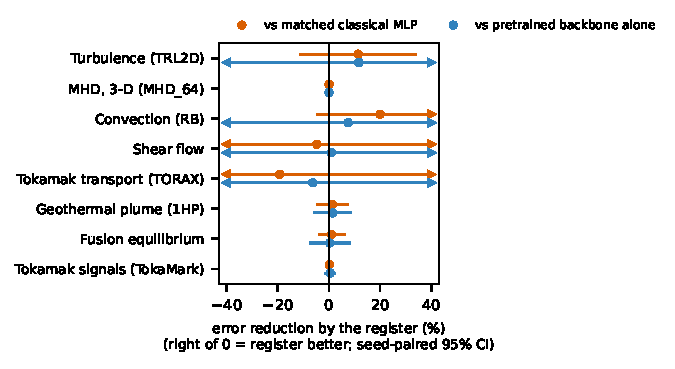
\includegraphics[width=0.55\linewidth]{fig_audit.pdf}}{}
\vspace{-14pt}
\caption{The audit at a glance: every 95\% interval of the register's seed-paired gain crosses zero.}
\label{fig:audit}
\vspace{-10pt}
\end{figure}
\begin{table}[h]
\centering
\caption{Matched-control audit, primary rows (three seeds unless noted; lower is better except Sophelio $S$).
Gains are seed-paired relative improvements of the register (positive $=$ better), with the number of seeds on which
the register is better and the paired $t$-test $p$. Metrics: VRMSE (@8: eighth rollout step), MAE in $^\circ$C,
official score $S$, NRMSE. CI: paired 95\% CI half-width of the register-vs-backbone gain (the effect just significant at $p<0.05$ given the observed spread; not a power-based MDE). Backbones: FNO (TRL2D arena), released CNextU-net (MHD\_64,
rayleigh\_benard, shear\_flow), 1-D spectral (TORAX-Bench), U-Net (heat plume, Sophelio starter), released TokaMind
(TokaMark). $^\dagger$Two length-matched seeds (Appendix~\ref{app:mhd}). $^\ddagger$Backbone tuned under the earlier
single-seed objective (mixed protocol). On rayleigh\_benard and shear\_flow, persistence ($\hat y_{t+1}=x_t$) scores
0.2024 and 0.0646, below every backbone and adapter in this table; the fix is in Appendix~\ref{app:gate}.}
\label{tab:auditfull}
\footnotesize
\setlength{\tabcolsep}{2pt}
\begin{tabular}{lccccccr}
\toprule
Benchmark & Backbone & $+$MLP & $+$Reg. & \multicolumn{2}{c}{Reg.\ vs MLP (\%)} & Reg.\ vs backbone (\%) & CI (\%) \\
\midrule
TRL2D arena & 0.9567 & 0.9534 & 0.8447 & $+11.4$ & 3/3, .16 & $+11.7$ 2/3 & 53 \\
MHD\_64$^\dagger$ & 0.1897 & 0.1897 & 0.1896 & $+0.0$ & 2/2, .28 & $+0.0$ 2/2 & 0.3 \\
rayleigh\_benard & 0.4563 & 0.5275 & 0.4221 & $+20.0$ & 3/3, .07 & $+7.5$ 1/3 & 69 \\
shear\_flow & 0.2686 & 0.2539 & 0.2659 & $-4.7$ & 2/3, .85 & $+1.0$ 2/3 & 99 \\
TORAX-Bench & 0.0158 & 0.0141 & 0.0168 & $-19.2$ & 0/3, .40 & $-6.4$ 2/3 & 84 \\
1HP heat plume$^\ddagger$ & 0.0291 & 0.0292 & 0.0288 & $+1.3$ & 2/3, .44 & $+1.2$ 2/3 & 5.2 \\
Sophelio $S$\,$\uparrow$$^\ddagger$ & 0.7905 & 0.7848 & 0.7929 & $+1.0$ & 2/3, .46 & $+0.3$ 1/3 & 7.5 \\
TokaMark 1-1 & 0.1509 & 0.1504 & 0.1501 & $+0.2$ & 1/3, .63 & $+0.5$ 2/3 & 1.8 \\
\midrule
\multicolumn{4}{l}{Rows better\,/\,worse\,/\,tied (sign-test $p$)} & \multicolumn{2}{c}{\AuditQvM{} ($p{=}\AuditQvMp$)} & \AuditQvT{} ($p{=}\AuditQvTp$) & \\
\multicolumn{4}{l}{Random-effects pooled gain [95\% CI]} & \multicolumn{2}{c}{\AuditREqm} & \AuditREqt & \\
\bottomrule
\end{tabular}
\end{table}
\label{app:audit}

The audit script reads every per-seed value from the result files rather than from summaries, fixes one primary row
per benchmark in advance, and reports per row the seed-paired gains, paired $t$, sign counts, $d_z$, Glass's
$\Delta$ and the paired 95\% CI half-width; across rows it reports a tie-aware sign test, the mean over rows with a
$t$ interval, and a DerSimonian--Laird random-effects pool with $I^2$ and leave-one-out values. Secondary rows:
MHD\_64 with all three seeds at unequal training length (register vs MLP $+4.2\%$, 3/3, $p=0.42$; flagged because four
of nine runs stopped at about 7.5k of 20k steps and at matched length the arms agree to four decimals with the gate
never opening, $|\alpha| \approx 4{\times}10^{-5}$); TORAX-Bench at fixed untuned hyperparameters (register vs backbone
$+9.1\%$, 3/3, $p=0.14$; vs MLP $+1.1\%$, 1/3); the heat plume at fixed hyperparameters (register vs MLP $+0.7\%$, 1/3);
Sophelio at fixed hyperparameters (register vs MLP $-0.2\%$, 1/3); TokaMark with a CNN backbone (one seed; register vs
backbone $+4.0\%$); and the TRL2D arena with a shared-link register ($+13.3\%$ vs MLP, 3/3, $p=0.20$). Three errors were
caught by the script before reaching a claim: the unequal-length MHD comparison above; a shear-flow published anchor
our evaluator does not reproduce (released checkpoint 0.9946 vs published 0.8080); and an inverse-variance pool that
rows with identical arms dominate, which is why the mean over rows and leave-one-out values are reported. Register
vs MLP leave-one-out pools range from $+0.16\%$ to $+2.16\%$, every interval including zero.

\section{Backbone architectures and insertion points}
\label{app:arch}
Figure~\ref{fig:overview} draws the TRL2D instance at layer level. Figure~\ref{fig:arch_backbones} draws the other
backbones of the audit (Table~\ref{tab:auditfull}) and of the comparison with published numbers
(Appendix~\ref{app:sota}) in the same way: feature maps as slabs labelled channels and grid size, fully connected
layers as bars labelled with their widths, Fourier and transformer layers as blocks. Shapes and parameter counts are
traced from the code and the released configurations (\texttt{paper/alloc/arch\_dump.py}). The register (orange) sits
at one latent per backbone. Where the latent is a field it is pooled first (the FNO before its projection, the
CNextU-net neck, the 1HP U-Net bottleneck, between the blocks of the TORAX-Bench spectral network); where the latent
is a vector it is read whole, with no pooling (the first hidden layer of the Sophelio starter UNetLite, TokaMind's CLS
token; \S\ref{sec:system}). Every write-back is zero-initialized and gated, so each hybrid starts at its released or
pretrained backbone. The routed co-processor (Fig.~\ref{fig:overview}, bottom) does not depend on the backbone: it
reads the backbone output and persistence and writes POD-mode corrections. The vehicle-routing solvers are described
in Appendix~\ref{app:routing}.

\begin{figure}[h]
\centering
\IfFileExists{fig_arch_backbones.pdf}{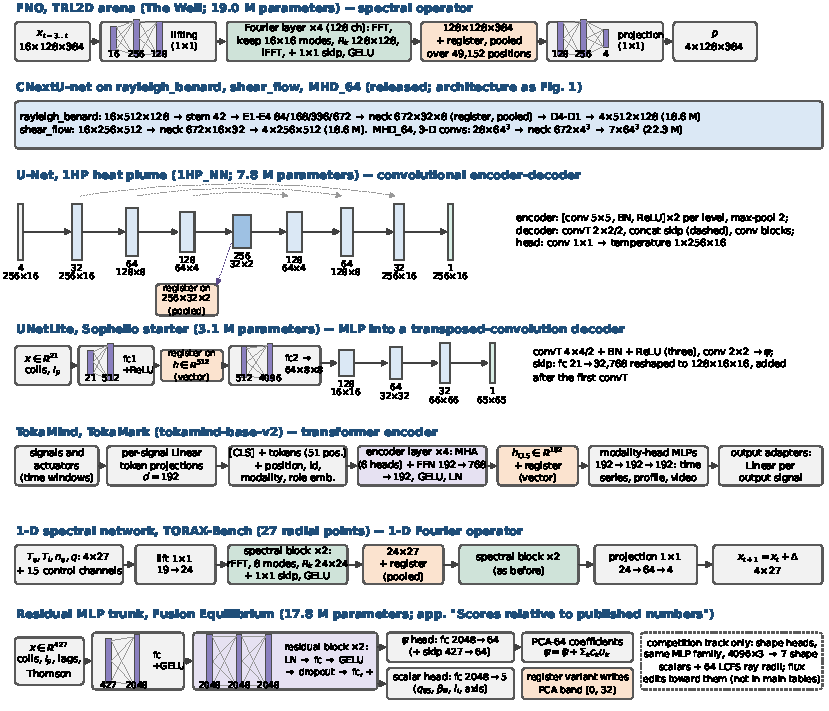
\includegraphics[width=\linewidth]{fig_arch_backbones.pdf}}{}
\caption{The other backbones at layer level, with tensor sizes, parameter counts and the register's insertion point
(orange). The shape heads in the last row's dashed box belong to the competition track only and enter no table of
the main text.}
\label{fig:arch_backbones}
\end{figure}

\section{Spectral evidence and machine-checked statements}
\label{app:spectral}

\begin{table}[h]
\centering
\caption{TRL2D (180 test windows): where the released checkpoint's error lives, by FFT shell $|k|$, and what the
register changes (paired over three Round-1 seeds, relative change of that shell's error energy vs vanilla).}
\label{tab:bands}
\small
\begin{tabular}{lcccc}
\toprule
$|k|$ shell & error energy share & change energy share & change missed by backbone & register vs vanilla \\
\midrule
0 (DC) & 0.029 & 0.022 & 0.23 & $-0.49\% \pm 0.21$ (3/3) \\
1--4 & 0.201 & 0.361 & 0.08--0.11 & within noise \\
5--16 & 0.428 & 0.459 & 0.11--0.21 & within noise \\
17--32 & 0.231 & 0.116 & 0.34 & within noise \\
$\ge$33 & 0.111 & 0.042 & 0.44--0.45 & within noise \\
\bottomrule
\end{tabular}
\end{table}




Both decompositions conserve energy (Haar relative error 0, FFT shells $2{\times}10^{-7}$). With Haar wavelets the
backbone misses 11\% of the change at the coarsest scale, rising to 18, 26, 32 and 37\% at 16, 8, 4 and 2 pixels; the
top 30 of 196{,}416 detail tiles per sample hold 32.9\% of the detail error energy, eleven times the DC ceiling, and a
zero-parameter router that ranks tiles by the backbone's own predicted change captures 9.4\% at $K{=}30$ (about 1{,}650
times a random choice); learned routers beat it only at $K \ge 3{,}000$. A routed register on TRL2D is a pilot
(Section~\ref{sec:limitations}).

\label{app:lean}
\paragraph{Machine-checked statements.} {\sloppy Lean~4 with Mathlib, standard axioms only (\texttt{propext},
\texttt{Classical.choice}, \texttt{Quot.sound}), no \texttt{sorry}: \texttt{pool\_blind} and \texttt{pool\_blind\_mode}
(mean pooling is invariant to zero-mean perturbations, in particular non-DC Fourier modes); \texttt{broadcast\_orthogonal};
\texttt{band\_energy\_split} and \texttt{residual\_after\_band\_removal} (Parseval split and the exact residual after a
perfect correction on a coefficient set, the ceiling of any $K$-tile corrector); \texttt{pointwise\_min\_optimal} and
\texttt{swap\_improves} (top-$K$ by energy is the optimal budgeted assignment); \texttt{reupload\_degree} (an $L$-layer
re-uploading circuit's spectrum lies in $[-L, L]$); \texttt{vdw\_sensitivity\_anti} (geometry acts as frequency
modulation); \texttt{lattice\_sep}; and \texttt{dip\_inplane}, \texttt{dip\_axial}, \texttt{dip\_magic} (signed dipolar
couplings require an out-of-plane coordinate); and, for the allocation study (\S\ref{sec:alloc}),
\texttt{gain\_le\_ceiling} (in any orthonormal basis, a correction supported on a coefficient set $T$, with arbitrary
coefficients, lowers the error energy by at most the error energy on $T$), \texttt{ceiling\_mono} (nested allocations
have nested ceilings), and \texttt{pooled\_gain\_le\_dc} (a spatially constant correction $c$ lowers
$\sum_i e_i^2$ by at most $(\sum_i e_i)^2/n$, whatever core and however many atoms produced $c$); and, for the
frequency-localized router and the persistence gate (Appendix~\ref{app:sota}), \texttt{band\_span\_le\_energy} (Bessel
inside a band: the energy on orthonormal band-localized modes never exceeds the band's energy, so captured$_b\le$
span$_b\le$ full$_b$ per band and window), \texttt{gate\_energy\_exact} and \texttt{gate\_coeff\_exact} (the gated
residual's energy and every mode coefficient are exact functions of three band statistics and two coefficients, for any
gate value), and \texttt{gate\_opt\_le} with its specializations \texttt{gate\_opt\_le\_persistence} and
\texttt{gate\_opt\_le\_trunk} (the best scalar gate per band is no worse than persistence or the backbone). The standard step that turns a parameterized circuit into a truncated
Fourier series is not formalized. A separate file checks algebraic consequences of a proposed configuration-aware
error model ($E = E_\infty + A P^{-\alpha}(1 - g\,u) + \dots$ with utilization $u \in [0,1)$): improvement with
utilization holds only when the signed gain $g \ge 0$, which is an empirical question the audit answers with a null.\par}

\section{Moving the insertion: protocols}
\label{app:move}

\paragraph{RealPDEBench.} Airfoil (NACA4418) real PIV velocity, 20 input and 20 output steps at $64\times128$; the
benchmark's public splits (5{,}133 validation and 5{,}140 test windows over 98 trajectories), normalizer and metric
code, with the full-set metric computed in exact chunks. The corrector reads the lowest $3\times4\times4$ space--time
modes of the backbone's prediction and of the last input window, standardizes them on the training split, passes them
through a zero-initialized gated core (none, linear, matched MLP, or 3$\times$10-atom register; the MLP and register
share input and output maps), and writes a correction to the same modes; it trains on training windows, early-stops
on validation relative $L_2$, and scores test once per arm and seed. The corrector does not exceed the released paper's
reported numbers, which are not reproducible on the current data release; the comparison is to the released checkpoint
evaluated with the benchmark's code.

\paragraph{Fusion Equilibrium Challenge.} Full-data pipeline (7{,}041 DIII-D shots, 1.56M frames; magnetics and Thomson
profiles; an extraction unit error placed the intended $-200$ to $+20$\,ms magnetics lags within 0.2\,ms, so these
models see no temporal context, Appendix~\ref{app:sota}), a PCA-64 flux decoder whose ground-truth projection scores $S = 0.9991$, and a stage-1
architecture search that fixed the frozen backbone. The stage-2 search over couplings (latent or spectral-routed,
register size and graph, $\le$30 atoms) ran on VALID only; its top three configurations were re-run with three seeds
beside matched MLP twins. Register vs MLP by configuration: 10-atom ring, learning rate $2.4{\times}10^{-3}$:
0.9878 vs 0.9876 ($p=0.43$); same register at $1.6{\times}10^{-3}$: 0.9878 vs 0.9868 ($p=0.030$, Bonferroni 0.09);
5-atom ring: 0.9879 vs 0.9876 ($p=0.41$). After the single registered test scoring (0.9910 on our held-out split of
training shots; the development leaderboard, which scores the public test fold, stood at 0.9932 in August and 0.9959 on
September 25), a
post-processing sweep on VALID only (shrinkage of high-order PCA coefficients, per-shot temporal smoothing, outlier
filters) raised the full-VALID score of the entry ensemble from 0.99127 to 0.99143. That is 1.7 times the estimated
ensemble seed SD, below the threshold we set in advance (3 times) for spending a second test scoring, so no second
test was run. The same selection rule, registered before the 3-D register results, was then applied to two further
pools and each selection scored once on the held-out split: classical trunks with the 3-D register models ($S$ 0.99100,
six members) and with their 3-D MLP twins (0.99099, seven). They tie each other and the classical-plus-MLP entry
(0.99102); the 3-D register selection is 0.0005 above the earlier 2-D register selection (0.99046), and the
classical-only selection scores 0.99097.

\section{Allocation study: protocol, per-strategy results and the analog--digital probe}
\begin{figure}[h]
\centering
\begin{minipage}[c]{0.52\linewidth}
\centering
\scriptsize
\setlength{\tabcolsep}{3pt}
\begin{tabular}{lcc}
\toprule
Register (fixed backbone) & Atoms & VRMSE@8 \\
\midrule
FNO backbone alone & 0 & \QLzero \\
$+$ Rydberg register & 5 & \QLfive \\
$+$ Rydberg register & 10 & \QLten \\
$+$ Rydberg registers & 20 & \QLtwenty \\
$+$ Rydberg registers ($3{\times}10$) & 30 & \QLthirty \\
\midrule
$+$ matched MLP (control) & --- & \QLmlp \\
$+$ 30 atoms, conditioned geometry & 30 & \QLgeo \\
$+$ 30 atoms, mean-field pilot & 30 & \QLgutz \\
\bottomrule
\end{tabular}
\end{minipage}\hfill
\begin{minipage}[c]{0.45\linewidth}
\centering
\IfFileExists{fig_scaling.pdf}{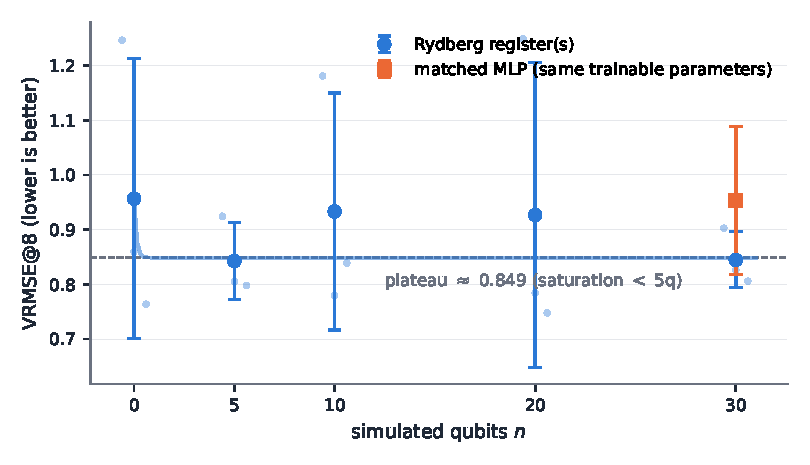
\includegraphics[width=0.85\linewidth]{fig_scaling.pdf}}{}
\end{minipage}
\caption{Rollout accuracy versus register size at fixed backbone, data and step budget (sprint arena, 3 seeds; amber:
matched MLP). The 0- and 30-atom arms ran first; the interior arms and the mean-field pilot were pre-registered before
execution. Points above 10 atoms add registers of 10. A constant fits the $n \ge 5$ points (a saturating fit puts
any rise below five atoms).}
\label{fig:scaling}
\end{figure}

\paragraph{Qubit count and inertness.} In a fixed-budget arena (FNO backbone, 2{,}000 steps), accuracy is flat from
five qubits: 5 atoms reach \QLfive{} against \QLthirty{} for 30 (Figure~\ref{fig:scaling}). The trained register is
inference-inert (product-state surrogates reproduce it within $2.4{\times}10^{-5}$), so any gain arises in training
(mechanism tests: Appendix~\ref{app:perseed}).

\label{app:alloc}

\paragraph{Caches and exactness.} Each frozen backbone predicts every window once (fp32; the convolutional and spectral
backbones have no layers NVFP4 applies to). Training windows are a uniform random sample of 3{,}000 (700 on the heat
plume); validation and test windows are uniform samples of all windows or the full split. For every window we store
the per-channel residual energy, the metric denominators, and, for 320 tiles per rule (proxy, static, random, oracle),
the Haar coefficients of $p - x_t$, $p$, $x_t$, $x_t - x_{t-1}$ and $r$. Because the transform is orthonormal, the
corrected per-channel error is $E_c - \sum_{i\in S}\big(r_{ic}^2 - (r_{ic} - c_{ic})^2\big)$ exactly, so VRMSE and
relative $L_2$ are computed without reconstructing fields; captured $\le U$ held on every cell. On the heat plume, the
"state" is the training-mean temperature field and the "change" is the permeability input, since the task is not
autoregressive; its study metric is VRMSE of the normalized temperature, not the benchmark's MAE.

\paragraph{Strategies and corrector.} A \emph{tile} is one Haar scale, orientation and position, all channels
together. \emph{Pooled}: global statistics in, one broadcast constant per channel out. \emph{Static}: the $K$ tiles
with the largest mean training error. \emph{Proxy}: top-$K$ by the energy of the backbone's own predicted change.
\emph{Learned}: a scorer trained to rank residual energy. \emph{Gain}: a scorer trained on the co-processor's own
realized per-tile gain. \emph{Random}. Atoms sit at their tiles ($x,y$ from position, $z$ from scale); detunings come from
tile features and global context. Each tile receives $c_i = s_i(W_{\kappa(i)} f_i + A\,o_i)$ with a per-(scale,
orientation) linear map $W$ shared by every arm, the core's readout $o_i = (\langle Z_i\rangle, \langle X_i\rangle,
\langle Y_i\rangle)$ and a zero-initialized $A$. With $A=0$ (the registered linear arm) the corrector alone gains 28.8\%
on rayleigh\_benard (proxy) and 26.3\% on shear\_flow (learned), test, three seeds; the cores' further 7.5 points on
rayleigh\_benard come from its heaviest-error windows (ranked by the backbone's error, the top 10\% carry 96\% of them; the median window changes by
$10^{-4}$), and on the other rows, at the listed tile strategies, the register adds at most 0.8 points (heat plume; MLP 1.0; 1.6 at
the heat plume's learned strategy). Input-adaptive routing adds 3.9 points to the linear corrector on shear\_flow but
none on rayleigh\_benard, where only the cores gain from it (3.4 register, 3.5 MLP). A registered replication with five new seeds (test windows reused) finds no register edge over the matched MLP on the convection-onset windows ($t_0<10$; MLP minus register $-0.09$ to $+0.06$ VRMSE, positive on 3/5 seeds), while both beat the classical mean-field twin there by 0.55--0.85 on every seed. The amendments: global context for tile co-processors after the
first cells; planetswe excluded because its released checkpoints do not reproduce.

\paragraph{Co-processor.} Tile features are scale-free (coefficients divided by the tile's own scale $s_i$, clipped),
plus log scale, scale and orientation one-hots, normalized position and the window's global statistics. Registers
are groups of 10 atoms in Morton (Z-order) order of their tiles; each atom's detuning per layer is
$b_{\ell i} + \pi\tanh(w_\ell^\top f_i)$ (weights shared across atoms), positions are tile coordinates divided by learned
per-axis blockade scales plus a learned scale-plane separation, and four layers of the propagator of
\S\ref{sec:system} are applied. The DeepSets MLP sees $[f_i, \bar f]$ and has the nearest width to the register's
parameter count (e.g.\ 316 vs 271 on TRL2D, 156 vs 165 on the heat plume). Scorers are two-layer MLPs trained with a
listwise loss over each window's proxy shortlist, on residual energy (learned) or on the proxy-trained co-processor's
realized per-tile gain (gain). AdamW, learning rate $3{\times}10^{-3}$, batch 64 windows, up to 40 epochs with patience 6
on validation; the loss is the negative captured share. A learning-rate check on TRL2D ($10^{-3}$ to $10^{-4}$) left the
TRL2D null unchanged.

\paragraph{Analog--digital probe.} Groups of 10 atoms with features $f_i \sim U[-1,1]^4$ on random sites of a
$4{\times}4{\times}2$ grid; targets per atom $\sin(\omega\, f_i^\top u)\cos(\omega\,\overline{f^\top v})$ (analog),
$\mathrm{sign}(f_i^\top u)\,\mathrm{sign}(\overline{f^\top v})$ (digital); 20k/5k/10k groups, Adam $3{\times}10^{-3}$, 3{,}000
steps, best-validation checkpoint, test $R^2$, three seeds. Registered rule: an analog edge requires the register to
beat its matched MLP on 3/3 seeds at $\ge 3$ of the five $\omega$. Test $R^2$, mean of three seeds ($^*$exploratory arms added after the $\omega \le 4$ results; MLP: nearest width to the register's 84 parameters, 75; MLP$^+$: next width up, 93):
\begin{center}\footnotesize\setlength{\tabcolsep}{3pt}
\begin{tabular}{lccccccc}
\toprule
core & $\omega{=}0.5$ & $\omega{=}1$ & $\omega{=}2$ & $\omega{=}4$ & $\omega{=}8$ & $\omega{=}16$ & digital \\
\midrule
register & 0.999 & 0.998 & 0.990 & 0.873 & 0.000 & -0.000 & 0.067 \\
mean-field & 0.803 & 0.971 & 0.990 & 0.642 & -0.000 & --- & 0.226 \\
MLP & 1.000 & 0.999 & 0.979 & 0.953 & -0.000 & -0.000 & 0.719 \\
MLP$^{+}$ & 1.000 & 1.000 & 0.989 & 0.956 & -0.000 & -0.000 & 0.920 \\
MLP$\times$4 & 1.000 & 1.000 & 0.986 & 0.989 & 0.012 & -0.000 & 0.954 \\
register, linear enc.$^*$ & --- & --- & --- & 0.874 & -0.000 & -0.000 & --- \\
sine-MLP$^*$ & --- & --- & --- & 0.988 & -0.000 & -0.000 & --- \\
\bottomrule
\end{tabular}\end{center}
Outside physics, on 22 TDC ADMET endpoints the register trails its matched MLP on \AllocTDC{}.

\paragraph{Caco-2 leader audit.}\label{app:caco2}
The Caco-2 leader (CaliciBoost, MAE 0.256) reproduces exactly with its released code (0.2560 $\pm$ 0.0060, five
seeds), but only with its hard-coded per-seed feature subsets and its GPU tree builder (CPU histograms: 0.271). TDC's
training and test sets do not change with the seed, yet the subsets do, and the code has no validation split. Without
selection the same model scores 0.294 $\pm$ 0.004; choosing the same number of features by permutation importance inside
the training data, as a method must, gives 0.308 $\pm$ 0.010. We list 0.256 as published, but it cannot be re-derived from
training data alone; our best, 0.276 (MapLight features and CheMeleon embeddings, CatBoost), is ahead of both re-derived values.

\paragraph{Positive control: quantum-generated targets.} Registered before any run, in the same harness: each atom's
target is $\langle Z_i\rangle$ after a 30-step Trotterized interacting Rydberg quench (constant drive $\Omega{=}1.5$,
input-set detunings $\delta_i{=}2f_i^\top u$, $V_{ij}{=}r_{ij}^{-6}$ with nearest neighbours at $V{\approx}1.8$). The
teacher's depth and fixed geometry lie outside the trained 4-layer ansatz. After a design critique, and before any register
result, we added message-passing cores that see the teacher's exact pair interactions. Test $R^2$ (three seeds):
mean-field register 0.671, register 0.433, GNN 0.333 and 0.357 (4$\times$), MLPs 0.19--0.20. The register beats
every MLP and GNN on every seed, so the harness separates cores sharply when the target calls for it. It loses to its
mean-field twin on every seed, however, so the registered rule is not met. What helps on these targets is the
Rydberg structure (geometry and $r^{-6}$ interactions), which the classical mean-field model carries. At ten atoms and
this training budget, entanglement adds nothing.

\section{Compute cost}
\label{app:compute}
All runs used one NVIDIA DGX Spark (GB10 Grace Blackwell chip, 128\,GB of unified CPU--GPU memory, Arm64 host); no cluster or cloud compute was used.
Median wall-clock per training step on the TRL2D neck insertion (released CNextU-net, $4\times16\times128\times384$
input, forward, backward and AdamW in float32, 25 steps after 5 warm-up, two repetitions, GPU shared with other jobs):
backbone 504\,ms, matched MLP 511\,ms, 30-atom register 595\,ms. The exact statevector propagator is the only added cost;
inference with a trained register can use its product-state surrogate at the MLP's cost because the trained register is
inference-inert.

\paragraph{Qubits are not parameters.} Every register--MLP comparison sizes the MLP from the register's parameter
count, never at one parameter per qubit (exactly in the neck audit; in the routed co-processor the integer hidden
width leaves the MLP smaller, as below). A 10-atom group evolves a $2^{10}=1{,}024$-amplitude state, but only its detuning maps, drives,
evolution times and coordinates are trained, and it returns three expectation values per atom, not its amplitudes. In the
routed co-processor on TRL2D at 30 qubits the register core has 244 parameters (241 trainable; its three length-scale
parameters are frozen) and its MLP 199, which
leaves the MLP two hidden units per atom. The qubit axis of Appendix~\ref{app:hscale} is therefore a different axis
from the parameter counts of classical world models: 30 to 50 qubits add a few hundred trainable parameters to a backbone
of 18.6 million (the TRL2D CNextU-net). That the register still ties an MLP with no more trainable parameters says these tasks, at these
sizes, do not draw on its larger state space.

\section{Scores relative to published numbers (all classical lifts)}
\label{app:sota}

\begin{table}[h]
\centering
\caption{Our best numbers against published ones. Every gain is attributable to classical components (the register effect on the TRL2D long-horizon row did not
replicate at four seeds, \S\ref{sec:trl2d}) (fine-tuning, correctors, ensembles,
edge-weighted training); the register's contribution is measured in Tables~\ref{tab:audit}--\ref{tab:move}.
Ensembles are labelled as such.}
\label{tab:sota}
\small
\setlength{\tabcolsep}{3pt}
\resizebox{\linewidth}{!}{%
\begin{tabular}{lllll}
\toprule
Benchmark & Published best & Released checkpoint, our evaluator & Persistence & Ours (component) \\
\midrule
TRL2D one-step VRMSE $\downarrow$ & Flowers 0.1930 (CNextU-net 0.1956) & 0.1934 & 0.5761 & \textbf{0.1909} (gated fine-tuning, 3-backbone ensemble; plain 3-seed ensemble 0.1929; Flowers' conditioned 1$\to$1 protocol: 0.1907) \\
TRL2D rollout 13:30 $\downarrow$ & CNextU-net 1.01 & 1.0132 & --- & 0.9528 (TD fine-tune with register, 3 seeds; 0.9660 with the registered fourth) \\
RealPDEBench foil rel.\ $L_2$ $\downarrow$ & released U-Net & 0.00948 & --- & 0.00931 (linear corrector $+$ 0.2 U-Net-real, VALID-weighted) \\
TokaMark 1-1 $\downarrow$ & TokaMind-Scratch 0.140 (FT-Base 0.150) & --- & n/a & 0.1334 (3 Scratch-recipe runs, equal weight, VALID-selected after the registered 4-member ensemble, 0.1400; one run 0.1379) \\
shear\_flow $\downarrow$ & PDE-FM 0.0345 (PhysiX 0.0700) & 0.9946 & 0.0646 & \textbf{0.0207} (gated classical part $+$ 30 routed qubits, 3 seeds; classical part alone 0.0236; with a metric-aligned loss 0.0197, 2 seeds, matched MLP 0.0199, seeds split 1--1) \\
rayleigh\_benard $\downarrow$ & PDE-FM 0.0415 (PhysiX 0.1470) & 0.6679 & 0.2024 & 0.0403 (gated, metric-aligned fine-tuning; equal-weight 3-backbone ensemble; best single model 0.0425; backbone alone 0.4563; 8-pass $x$-symmetry average 0.0366$^\dagger$) \\
Fusion Equilibrium Ch.\,1 $S$ $\uparrow$ & 0.9959$^\ast$ & --- & n/a & TEST 0.9949 (VALID-selected 7-member ensemble \SophTEST{}, VALID 0.9913; with registered shape-head post-processing and a $\psi$-specialist ensemble as described below; still below the best) \\
\bottomrule
\end{tabular}}
\end{table}

$^\ast$Fusion Equilibrium: best development-leaderboard entry on the public DIII-D test fold, September 25, 2026 (0.9932 in August). Our TEST is a held-out split of the training shots, not the same test set.
MHD\_64's released checkpoint evaluates to 0.5447 per-channel VRMSE, not the published 0.1633 (our gated, fine-tuned
backbone: 0.1725 on the full test split; current best 0.1160, EddyFormer. A Flowers model trained from scratch with the authors' schedule scores 0.1216 (their 0.1165); with the divergence-free and conserved-mean projections 0.1191, after a 5-epoch fine-tune on the VRMSE itself 0.1172, and blended with the gated CNextU-net by channel and band (weights fit on TRAIN) 0.1154, which we call parity; symmetry averaging, 8$\times$ inference, gives 0.1035$^\dagger$. In the CNextU-net model, its error is regime-level, not a tail: over the two
fine-tuned CNextU-net seeds trained to full length the five super-Alfv\'enic test runs, $M_A{=}2$, score 0.217--0.218 against
0.136--0.137 at $M_A{=}0.7$ (61\% of the error), flat in time, and the worst 10\% of windows hold 14\% of the mean, which leaves routed modes little to reach), and shear\_flow's to
0.9946, not 0.8080; on shear\_flow we therefore compare with the foundation models PDE-FM \citep{soares2025pdefm} and
PhysiX \citep{nguyen2025physix}, which report full official test splits without ensembles or test-time augmentation,
and not with the released checkpoint. Our classical part alone (0.0236, full test split) is below PDE-FM's 0.0345; on
rayleigh\_benard our ensemble (0.0403) is within 3\% of PDE-FM's single model (0.0415), which we call parity, not a win; our best single model scores 0.0425 (its first test score), 2.3\% above it. Averaging each model over the exact symmetries of the periodic cell (reflection $x\to-x$ with $u_x\to-u_x$, times four periodic shifts; $^\dagger$8$\times$ inference, registered before its test score) gives 0.0383 for the single model and 0.0366 for the ensemble ($-9.8\%$ and $-9.1\%$, paired over test trajectories, 95\% CIs within $\pm0.8$ points); PDE-FM reports a single pass. The gap between the register and the matched MLP neck (one checkpoint each, seed 1337: 0.0425 vs 0.0438, $-3.1\%$) shrinks to $-0.8\%$ under the same averaging (0.0383 vs 0.0386); it is one checkpoint pair, not a training replication (the multi-seed tests are in Appendix~\ref{app:hscale}).
Training protocols differ (per-dataset fine-tuning here, cross-physics pre-training there) and are not normalized.
Persistence ($\hat y_{t+1}=x_t$, full official test splits, the benchmark's own mean VRMSE) is a necessary baseline on
the Well rows: it scores 0.2024 on rayleigh\_benard and 0.0646 on shear\_flow, below The Well's published baselines,
PhysiX on shear\_flow (0.0700) and every backbone we trained (0.36--0.57 and 0.22--0.34), though not PDE-FM, although the backbones win 84\% and 54--63\% of the individual windows; their
mean is dominated by a heavy tail of low-variance windows. On TRL2D (0.5761) and MHD\_64 (0.4183, beaten on every window) the backbones are far
better than persistence. We therefore make no state-of-the-art statement from backbone numbers on rayleigh\_benard or
shear\_flow. With the band gate and metric-aligned fine-tuning (Appendix~\ref{app:gate}), rayleigh\_benard reaches 0.0403 on
the full test split, a fifth of persistence. This reflects metric alignment, not better convective dynamics: the
convection-onset windows ($t_0<10$, 3.6\% of test windows) carry 39\% of the backbone's mean VRMSE (backbone 4.86,
persistence 0.038 on them), and the classical gate leans on persistence per band and window where the backbone is unreliable. Recent foundation and compact models on The Well \citep{mccabe2025walrus,sankaran2026wavelit} report the
\emph{median} one-step VRMSE over windows, not the benchmark's mean. Because the mean is dominated by the heavy tail
discussed above, their numbers are not comparable to the mean-based scores in this table.

\paragraph{Where TokaMark 1-1 is lost.} Training TokaMind from scratch with its published recipe gives 0.1379 in our
evaluator (one seed), matching the reported 0.140; the registered equal-weight ensemble of this model with three
fine-tuned FT-Base seeds gives 0.1400: the FT-Base members (0.150--0.151 each) hold three of the four equal weights and dilute
the Scratch model. We report this registered ensemble as is. After it, a stratified VALID diagnosis (534 shots) selected
the equal-weight ensemble of the three Scratch-recipe runs below (vanilla, MLP neck, register neck; one seed), registered
before its TEST score: 0.1334, $-3.2\%$ against the single run (paired over 1{,}020 test shots, 95\% CI 2.9--3.6\%,
829 shots better); adding the three FT-Base runs with per-feature weights fit on TRAIN gives 0.1332, not resolved from it ($-0.17\%$, CI $-0.41$ to $+0.07\%$). It is post hoc with respect to the registered ensemble and credits neither neck. With the neck swapped
at the same slot on the Scratch recipe (one seed each), the register neck gives 0.1404 and the MLP neck 0.1391: neither
helps this backbone. On the FT-Base recipe the 3-D tethered register (full recipe, one seed) scores 0.1512 against 0.1500
for its matched MLP (2{,}178{,}573 and 2{,}178{,}411 parameters) and 0.1504 without a neck; the MLP is lower on 13 of the 15 signals
(one seed, descriptive). The registered ensembles tie: 0.1400 (vanilla), 0.1400 (register neck), 0.1402 (MLP neck). Per target, our 3-seed register-neck FT-Base ensemble (0.1454 overall) beats
TokaMind-Scratch (0.140; per-target values from its Table A.2 \citep{boschi2026tokamind}) on the plasma geometry:
$x$-point $z$ 0.0201 vs 0.022, $x$-point $r$ 0.1654 vs 0.170, magnetic-axis $z$ 0.0725 vs 0.075. The whole gap is in the
three pressure ratios: $\beta_{\mathrm{pol}}$ 0.1655 vs 0.153, $\beta_N$ 0.1687 vs 0.157, $\beta_{\mathrm{tor}}$ 0.1680
vs 0.157. The vanilla and MLP-neck ensembles show the same pattern. By shot length, the mean per-shot NRMSE is 0.172
on the shortest quarter of test shots ($\le$218 windows, mostly early terminations) against 0.131--0.141 on the rest,
so the gap is concentrated in short, disrupted discharges. It is not a learnable bias. On the test windows, the share of
the $\beta$ squared error explained by its mean within bins of shot length $\times$ time in shot is at most 0.6\% (an
in-sample upper bound for any additive correction on those bins), and the reconstructed $\beta$ labels jump 1.5--9.6$\times$
more than the predictions between consecutive windows. We read this as noise in the EFIT labels near termination and
fit no correction; the rule was fixed before the numbers.

\paragraph{Where the Fusion Equilibrium score is lost.} On full VALID, $1-S=0.0088$ for the entry; the consistency
term (shape scalars derived from the predicted flux: elongation, internal inductance, volume, axis position) carries
75\% of it, the LCFS distance 17\%, $\psi$ 2\%. Two input errors surfaced in a stratified diagnosis: our magnetics
lags were sub-millisecond (above), and on the 20\,kHz shots (70\%) the challenge's shared plasma-current time vector
reads $|I_p|<5\%$ of its peak at 57--100\% of EFIT frames, which cannot hold during a plasma; anchoring it to the
magnetics clock removes this (pre-breakdown $|I_p|$ median 0.2\% of peak). A matched retrain of the entry's best trunk
(two seeds, 180 stratified VALID shots, official $S$) registered before running shows that neither correction helps:
the re-anchored current alone lowers $S$ by 0.0011--0.0017 (95\% CIs below zero); with the true-ms lags as well, pooled
$\psi$ and scalar-head $R^2$ improve on both seeds but $S$ changes by $-0.0006$ and $-0.0005$ (CIs span zero), because
the flux-derived shape consistency worsens; a second registered pass (an explicit acquisition-rate input; lags floored at $-50$\,ms) lowers $S$ further. The entry is therefore not retrained, and the gap to the best
development-leaderboard entry (0.9959) stays open.

\paragraph{Where the Fusion Equilibrium score is recovered.} Most of the consistency loss comes from extraction, not the flux map: the true $\psi$ projected on the 64 PCA components scores $S=0.9991$, and our predicted map has $R^2_\psi=0.9997$, yet the shape scalars derived from it lose 3\%. The scorer reads the magnetic axis as a sub-pixel critical point (the $Z_{\rm axis}$ spread, 0.043\,m, is below one 0.05\,m cell) and the boundary through the X-point, so small flux errors near critical points are amplified. Direct heads trained on the scorer's own extraction of the training-split flux (from its stored 256-component form; no validation or test labels) beat the shape extracted from our predicted flux on 180 stratified VALID shots: $R^2$ 0.991 vs 0.978 for $Z_{\rm axis}$ (the trunk's own head), 0.965 vs 0.933 for elongation, 0.987 vs 0.966 for volume, boundary radius error 7.1 vs 9.9\,mm. Registered inference-only edits move the predicted flux so that the scorer's extraction lands on the heads. The plasma core is shifted (Gaussian window, zero at the boundary) until the scorer's O-point finder returns the head axis. The flux is warped radially about the axis so that the extracted boundary meets the head radii, leaving the far field fixed. An area-preserving elongation about the boundary's centre matches the scorer's elongation to its head. Finally the interior flux profile is remapped toward the internal-inductance head, keeping the axis, boundary level and boundary gradient. Each step was picked on VALID and scored once on our held-out TEST split (373 shots): $S$ $0.99102\to0.99155$ (axis), $\to0.99159$ (inductance; a weak replication, $+0.00003$ against $+0.00018$ on VALID), $\to0.99251$ (boundary), $\to0.99291$ (heads retrained on all training frames with gradient clipping, after unclipped long runs diverged in 2 of 3 seeds), $\to0.99323$ (elongation) and $\to0.99339$ (heads trained twice as long with the seven scalars weighted equal to the 64 boundary radii) $\to0.99343$ (six head seeds) and $\to0.99369$ (flux from three $\psi$-only trunks, trained without the scalar loss, each step re-scored on a GPU port of the post-processing that matches the CPU one under the official scorer) $\to0.99490$ (inputs with the plasma current re-timed on 20\,kHz shots and lags in true milliseconds, for the $\psi$ trunks, the $q_{95}$/$\beta_N$ trunks and the heads, plus a lateral warp of the top and bottom points toward the triangularity heads; the warp alone adds $+0.00005$). Elongation $R^2$ rises from 0.931 to 0.959, volume from 0.968 to 0.984, and the boundary distance falls from 0.0146 to 0.0119. Dedicated $q_{95}/\beta_N$ heads, finer boundary sampling at fixed head quality, and a triangularity shear did not help. The leaderboard file stores $\psi$ in float16, as the starter kit recommends; on VALID that alone costs 0.0004 (the same with and without the edits), so float32 storage is the exact fix.

\section{Confirmatory and exploratory claims}
\label{app:claims}

Every final configuration was scored on TEST once, but most protocols were designed after earlier TEST results on the
same rows were known (new seeds or budgets on the same test windows included), so TEST was reused adaptively across
amendments and only the first audit round is confirmatory. Table~\ref{tab:claims} labels each claim.
\emph{Confirmatory}: the decision rule and the TEST sample were fixed before any TEST result on that row.
\emph{Registered, TEST-informed}: the rule was fixed before the run, but the design followed earlier TEST results on
the same rows; these claims are exploratory. \emph{Descriptive}: no decision rule. A prospective test on benchmark rows
not used elsewhere in this paper (active\_matter and gray\_scott\_reaction\_diffusion; TEST downloaded only after the
prediction, the 24 trained models and the rule were locked and hashed; each model scored once) predicted from VALID that
error-proxy routing beats pooled insertion in both the register and a matched MLP core. It held on both rows: mean
seed-paired TEST gains 12.3\% (register) and 14.1\% (MLP) on active\_matter, 15.2\% and 24.8\% on gray\_scott
(trajectory-bootstrap 95\% intervals above zero). The MLP gained more than the register on both rows, so this supports this
operational proxy-insertion strategy on these rows, not a quantum advantage; it does not isolate routing from the
insertion architecture, and the gain is concentrated (two of 21 active\_matter configurations give about 80\% of the
absolute improvement; gray\_scott's gliders about 90\%). Post hoc, on the gray\_scott V2 half of VALID an earlier, separately trained linear-only tile
corrector of the same recipe scored below the register-based corrector on all three seeds, and removing the core term
from the frozen register checkpoints also lowered V2 error on all three seeds. On gray\_scott the proxy arm has about 60\% fewer co-processor
parameters than pooled; on active\_matter it has about 53\% more.

\begin{table}[h]
\centering
\caption{Status of each claim. Rows in the order of the main text.}
\label{tab:claims}
\footnotesize
\setlength{\tabcolsep}{3pt}
\begin{tabular}{p{0.47\linewidth}p{0.2\linewidth}p{0.27\linewidth}}
\toprule
Claim & Status & Where \\
\midrule
Pooled neck register ties its matched core on eight benchmarks & confirmatory & \S\ref{sec:audit}, Table~\ref{tab:audit} \\
TRL2D long-horizon edge does not replicate at a fourth seed & TEST-informed (negative) & \S\ref{sec:trl2d} \\
Frequency gate beats persistence and the backbone & TEST-informed & \S\ref{sec:move}, Appendix~\ref{app:gate} \\
Routing gains 26\%/36\% vs 7\% pooled (linear corrector alone 26\%/29\%); matched cores gain as much & TEST-informed & \S\ref{sec:alloc}, Table~\ref{tab:alloc} \\
Error falls with the budget; bounds at 50, 100, 200 qubits hold & TEST-informed ($U$ from test labels) & \S\ref{sec:alloc}, Appendix~\ref{app:hscale} \\
Register beats a smaller graph-blind MLP (199 vs 244 parameters) at 100 qubits on shear flow (5/5 new seeds), not established against a graph-aware GNN (239) or a wider MLP (297) & registered replication, TEST-informed & Appendix~\ref{app:hscale} \\
Closed form $G(K)$; captured share $\le U$ (an algebraic check) & descriptive & \S\ref{sec:alloc} \\
Tested per-input geometry, tethers and 3-D layout did not meet the registered gain rule & TEST-informed (negative) & Appendix~\ref{app:hscale} \\
3-D register vs its matched MLP per benchmark & TEST-informed; no two-sided test passes & Appendix~\ref{app:hscale} \\
Probabilistic hybrid: lower proper energy score than the deterministic hybrid and a VALID-tuned dressing (shear\_flow, rayleigh\_benard; 3/3 seeds; matched MLP equal) & registered & Appendix~\ref{app:fgn} \\
Scores against published numbers & descriptive & Appendix~\ref{app:sota} \\
Routing gains are predictable from validation data on unseen rows & confirmatory, pending & registered \\
\bottomrule
\end{tabular}
\end{table}

\section{Evaluation-error analysis: persistence, a frequency-aware gate, and metric-aligned fine-tuning}
\label{app:gate}

\paragraph{Where the Well backbones fail.} The benchmark's score is the mean over windows of a per-window, per-field
VRMSE, which divides each window's error by that window's variance. On rayleigh\_benard and shear\_flow this mean is
dominated by a heavy tail of low-variance windows (early convection onset; slowly evolving shear layers). There the
backbones, trained with plain MSE on normalized fields, give those windows almost no weight. Persistence
($\hat y_{t+1}=x_t$) is therefore a strong baseline: on the full official test splits it scores 0.2024 and 0.0646,
below The Well's published baselines (0.6566, 0.8080) and every backbone we fine-tuned, though not PDE-FM (0.0415, 0.0345), although the backbones win 84\% and
54--63\% of individual windows. A per-window oracle choice between backbone and persistence would score 0.044--0.048 and
0.036--0.039. On TRL2D (0.5761) and MHD\_64 (0.4183) persistence is far behind.

\paragraph{A classical, frequency-aware gate.} A related classical design in Hybrid Neural World Models
\citep{lakshmanan2026hnwm} gates a neural surrogate against a reference-solver fallback using an error map that detects
sharp dynamical events (shocks, fronts). In our architecture, the fallback is persistence, evaluated per window and
Fourier octave; rather than abandoning surrogate throughput via an expensive numerical solver fallback, QUOTA routes the
remaining frequency-localized residual modes directly to an agile quantum (or matched classical) co-processor. We split
the backbone's increment over persistence into five dyadic
$\ell_\infty$ Fourier shells $P_b$ (orthogonal projectors summing to the identity) and predict
$\hat y = x_t + \sum_b \alpha_{c,b}\,P_b\big(p(x) - x_t\big)$ per field $c$. With $\alpha$ fitted in closed form on
training windows (the \emph{blend}) or predicted per window from causal features (the \emph{gate}: band energies of
$p-x_t$ and of the last input increment, normalized by the last input frame's variance), the gated residual's energy
and every mode coefficient are exact functions of cached band statistics (\texttt{gate\_energy\_exact},
\texttt{gate\_coeff\_exact}; the per-band oracle gate is no worse than persistence or the backbone,
\texttt{gate\_opt\_le}). The blend keeps the backbone's low bands and falls back to persistence for the high bands of
the velocity fields ($\alpha\approx1$ at low $k$, $0$--$0.1$ at the top octave). A first version normalized the gate's
features by the \emph{target} frame's variance. We caught this leak, archived those runs, and reran with causal features.
Every number below is causal; the change moved results by less than 1\%.

\paragraph{The routed register after the gate.} The residual that remains is written in band-wise POD modes (POD
computed inside each band, so each qubit carries a signal of known band, and per band captured$_b\le$ span$_b\le$
full$_b$ holds for every window, \texttt{band\_span\_le\_energy}). A learned router sends 30 modes per window to the
register, and a classical head takes the rest. Without supervision, the router left the register nearly idle: it put 92\% of its slots in
the top octave, which holds almost none of the reachable error. Supervising the router toward each window's largest
reachable error moved 80\% of the slots to the lowest band. Table~\ref{tab:gate} reports the matched cores
(register, GNN on its own learned graph, MLP) with the supervised router. With supervision, routing matches the allocation
thesis: the qubit-routed modes carry most of the co-processor's capture, in the band where the reachable error is
(Table~\ref{tab:gatebands}). But the matched classical cores, each behind its own separately trained router of the same design, capture as much: the cores
tie (the register's and MLP's routed sets overlap by 40\% on shear\_flow, seed 1).
We attribute the gains to the gate, the routing and the classical head.

\begin{table}[h]
\centering
\caption{Evaluation-error analysis on the Well rows (VRMSE, lower is better). Published: best published number (PDE-FM
on shear\_flow and rayleigh\_benard, Flowers 4$\to$1 on TRL2D, EddyFormer on MHD\_64). Backbone: the fine-tuned (or released) CNextU-net. Blend: TRAIN-fitted band blend with persistence. Gate: per-window causal band gate. The last three
columns stack the routed co-processor (30 atoms or matched classical cores) on the gate; mean\,$\pm$\,SD over seeds.
Full official test splits except $^\dagger$ (stratified test sample, every trajectory $\times$ 8 time bins, 4
windows each; validated against full-split per-window scores to within 2\%). The Well's CNextU-net claims 0.1633 on
MHD\_64; its released checkpoint evaluates to 0.5447.}
\label{tab:gate}
\scriptsize
\setlength{\tabcolsep}{2pt}
\resizebox{\linewidth}{!}{%
\begin{tabular}{lcccccccc}
\toprule
Row (backbone) & Published & Persistence & Backbone & Blend & Gate & $+$Register & $+$GNN & $+$MLP \\
\midrule
%GATE-ROWS-BEGIN
shear\_flow (register neck) & 0.0345 & 0.0646 & 0.2297 & 0.0451 & 0.0272 & 0.0201\,$\pm$\,0.0002 & 0.0205\,$\pm$\,0.0002 & 0.0200\,$\pm$\,0.0003 \\
rayleigh\_benard$^\dagger$ (register neck) & 0.0415 & 0.2024 & 0.4321 & 0.1420 & 0.0420 & 0.0413 & 0.0415\,$\pm$\,0.0003 & 0.0416\,$\pm$\,0.0004 \\
rayleigh\_benard$^\dagger$ (vanilla) & 0.0415 & 0.2024 & 0.4252 & 0.1438 & 0.0436 & --- & --- & --- \\
TRL2D (register neck) & 0.1930 & 0.5761 & 0.1931 & 0.1924 & 0.1921 & 0.1922 & 0.1922\,$\pm$\,0.0001 & 0.1922 \\
TRL2D (released) & 0.1930 & 0.5761 & 0.1934 & 0.1926 & 0.1924 & 0.1923\,$\pm$\,0.0001 & 0.1923\,$\pm$\,0.0001 & 0.1923\,$\pm$\,0.0001 \\
MHD\_64 (vanilla) & 0.1160 & 0.4183 & 0.1771 & 0.1761 & 0.1735 & 0.1733 & 0.1733 & 0.1733 \\
%GATE-ROWS-END
\bottomrule
\end{tabular}}
\end{table}

\begin{table}[h]
\centering
\caption{Where the register's work goes, per Fourier band, after the gate (route-supervised router, seed 1). Shares of
each window's error before the gate, averaged over test windows. full$_b$: error in band $b$ after the gate.
span$_b$: part of it on the band's POD modes. Then what the qubit-routed modes and the classical head capture, and
the share of the 30 qubit slots that land in the band. The chain captured$_b\le$ span$_b\le$ full$_b$ is checked on
every window; the largest violations are fp16 rounding.}
\label{tab:gatebands}
\scriptsize
\setlength{\tabcolsep}{4pt}
\begin{tabular}{llccccc}
\toprule
Row & Band & full$_b$ & span$_b$ & Captured (qubits) & Captured (classical) & Qubit slots \\
\midrule
%BAND-ROWS-BEGIN
shear\_flow & $b_0$ & 0.3891 & 0.3433 & 0.2167 & 0.0419 & 95\% \\
 & $b_1$ & 0.0444 & 0.0186 & 0.0050 & 0.0008 & 2\% \\
 & $b_2$ & 0.0360 & 0.0080 & 0.0005 & 0.0000 & 3\% \\
 & $b_3$ & 0.0297 & 0.0016 & -0.0000 & -0.0004 & 0\% \\
 & $b_4$ & 0.0342 & 0.0006 & 0.0000 & -0.0002 & 0\% \\
& \multicolumn{6}{l}{max violation: captured$\le$span -1.5e-10, span$\le$full -5.3e-08} \\
rayleigh\_benard & $b_0$ & 0.0476 & 0.0359 & 0.0186 & 0.0011 & 81\% \\
 & $b_1$ & 0.0180 & 0.0047 & 0.0008 & 0.0001 & 12\% \\
 & $b_2$ & 0.0151 & 0.0017 & 0.0009 & 0.0000 & 2\% \\
 & $b_3$ & 0.0191 & 0.0008 & 0.0007 & -0.0000 & 1\% \\
 & $b_4$ & 0.0267 & 0.0008 & 0.0004 & 0.0000 & 3\% \\
& \multicolumn{6}{l}{max violation: captured$\le$span -3.2e-09, span$\le$full -6.0e-07} \\
%BAND-ROWS-END
\bottomrule
\end{tabular}
\end{table}

\paragraph{Metric-aligned end-to-end fine-tuning.} The fix belongs in training, not only in stacking. We fine-tune the
whole stack end to end: backbone (vanilla, MLP neck, or register neck), gate, and the benchmark metric itself as the loss.
Selection uses a stratified validation sample; the selected configuration is scored once on the full test split
(Table~\ref{tab:ft}).

\begin{table}[h]
\centering
\caption{End-to-end fine-tuning with the band gate (seed 1). Loss: VRMSE (the benchmark metric) or MSE. Schedule:
joint from the start, or exact gate pre-training on 3{,}000 frozen-backbone training windows, then joint. VALID:
stratified sample (start $\to$ best). Test: stratified estimate, and the full split for the selected cells.}
\label{tab:ft}
\scriptsize
\setlength{\tabcolsep}{3pt}
\begin{tabular}{lllllcccc}
\toprule
Row & Backbone & Loss & Head & Schedule & VALID start & VALID best & Test (strat.) & Test (full) \\
\midrule
%FT-ROWS-BEGIN
shear\_flow & MLP neck & vrmse & gate & pre & 0.0284 & 0.0284 & 0.0280 & --- \\
shear\_flow & register neck & vrmse & gate & pre & 0.0275 & 0.0275 & 0.0271 & --- \\
shear\_flow & 3-D register neck & vrmse & gate & pre & 0.0307 & 0.0307 & 0.0302 & 0.0303 \\
shear\_flow & 3-D MLP neck & vrmse & gate & pre & 0.0286 & 0.0286 & 0.0281 & --- \\
shear\_flow & vanilla & vrmse & gate & pre & 0.0301 & 0.0294 & 0.0298 & --- \\
rayleigh\_benard & MLP neck & vrmse & gate & joint & 0.1436 & 0.0681 & 0.0659 & --- \\
rayleigh\_benard & MLP neck & vrmse & gate & pre & 0.0454 & 0.0437 & 0.0438 & --- \\
rayleigh\_benard & register neck & mse & gate & joint & 0.1426 & 0.1426 & 0.1415 & --- \\
rayleigh\_benard & register neck & vrmse & gate & joint & 0.1426 & 0.0777 & 0.0742 & --- \\
rayleigh\_benard & register neck & vrmse & gate & pre & 0.0422 & 0.0422 & 0.0425 & --- \\
rayleigh\_benard & register neck & vrmse & plain & joint & 0.4470 & 0.4470 & 0.4331 & --- \\
rayleigh\_benard & 3-D register neck & vrmse & gate & pre & 0.0425 & 0.0425 & 0.0429 & 0.0428 \\
rayleigh\_benard & 3-D MLP neck & vrmse & gate & pre & 0.0423 & 0.0423 & 0.0426 & 0.0426 \\
rayleigh\_benard & vanilla & vrmse & gate & joint & 0.1441 & 0.0891 & 0.0854 & --- \\
rayleigh\_benard & vanilla & vrmse & gate & pre & 0.0438 & 0.0438 & 0.0441 & --- \\
TRL2D & MLP neck & vrmse & gate & pre & 0.1930 & 0.1918 & 0.1922 & --- \\
TRL2D & register neck & vrmse & gate & pre & 0.1928 & 0.1919 & 0.1921 & --- \\
TRL2D & vanilla & vrmse & gate & pre & 0.1926 & 0.1916 & 0.1921 & --- \\
MHD\_64 & register neck & vrmse & gate & pre & 0.1723 & 0.1714 & 0.1728 & --- \\
MHD\_64 & vanilla & vrmse & gate & pre & 0.1722 & 0.1714 & 0.1727 & --- \\
shear\_flow & E-ft (3 backbones, equal) & vrmse & gate & pre & --- & 0.0256 & --- & 0.0252 \\
rayleigh\_benard & E-ft (3 backbones, equal) & vrmse & gate & pre & --- & 0.0400 & --- & 0.0403 \\
TRL2D & E-ft (3 backbones, equal) & vrmse & gate & pre & --- & 0.1917 & --- & 0.1909 \\
MHD\_64 & E-ft (2 backbones, equal) & vrmse & gate & pre & --- & 0.1726 & --- & 0.1725 (vanilla) \\
%FT-ROWS-END
\bottomrule
\end{tabular}
\end{table}

Three readings. First, the closed-form gate on the frozen backbone already captures the gain. After exact gate
pre-training, the joint stage improves VALID by at most 0.001, and on shear\_flow the best checkpoint is the starting
one, so end-to-end retraining is not needed. Second, the loss matters only together with the gate. On
rayleigh\_benard, MSE with the gate gives 0.1415, VRMSE without the gate 0.4331, and both together 0.0425--0.0742. The
VRMSE loss gives low-variance onset windows the gradient that MSE takes away; the credit goes to that classical loss,
not to the neck. Third, the three backbones tie within one seed (TRL2D 0.1921--0.1922, MHD\_64 0.1727--0.1728), and no
register edge is claimed from the single-seed differences on rayleigh\_benard and shear\_flow.
The registered equal-weight ensemble of the three backbones (E-ft; registered before any ensemble score) is chosen on
VALID over the best single backbone on rayleigh\_benard (0.0400 vs 0.0422) and scores 0.0403 on the full test split. The
members' residual fields correlate at 0.59--0.64, symmetrically across pairs, so the gain is ordinary variance
reduction; the register neck is one member and gets no credit for it. On MHD\_64 the two members' residuals correlate
at 0.999, the ensemble ties them on VALID, and the selected single backbone scores 0.1725 on the full test split.
On shear\_flow (residual correlations 0.49--0.68) E-ft is selected and scores 0.0252 on the full test split. On TRL2D it is selected by 0.0001 on VALID
and scores 0.1909 on the full test split, below the CNextU-net's 0.1956 and 1\% below Flowers' 0.1930 \citep{muser2026flowers}. There the members' residuals correlate at
0.997--0.999, which bounds the ensembling gain at about 0.0001, so the step from the frozen-backbone gate (0.1921,
Table~\ref{tab:gate}) to 0.1909 comes from the gated, metric-aligned fine-tuning itself.

\paragraph{What is left: a transform diagnosis.} We decomposed the final models' test error per Fourier octave, per
Haar wavelet level and by one-step lag regression (Figure~\ref{fig:spectral}; diagnostics only, with no model parameters updated). With $D=y-x_t$ the true change and
$P=\hat y-x_t$ the predicted change, the magnitude-squared coherence of $P$ and $D$ in an octave gives its Wiener floor,
the least error any spatially uniform linear gain on $P$ in that octave can reach. On rayleigh\_benard the models sit on
this floor in every octave and field; on TRL2D they are within 0.06 of it (in units of the octave's true-change energy);
adding the last observed change $x_t-x_{t-1}$ as a second regressor lowers the floor by at most 0.03. Neither the
tested scalar gain nor this two-regressor filter removes what is left; longer-lag or cross-field linear filters, and
nonlinear, cross-scale or local models, might. In the temporal diagnostic, the model's lag-one regression slope of each octave's next change on its last observed change (teacher-forced,
one step; not the model's own pole) matches the true slope within 0.02 on TRL2D and rayleigh\_benard; in the
top octaves both sit near $-\tfrac12$, the value that frame-to-frame white content gives (differenced i.i.d. noise gives exactly
$\mathrm{corr}(D_{t+1},D_t)=-\tfrac12$, and approximately so when the signal's own changes are negligible). On shear\_flow the models' slope there is near 0 against the
truth's $-0.43$ to $-0.51$, the one mismatch we found. Wavelets locate the error: on TRL2D 98\% of its energy lies in
5\% of the Haar coefficients, along the mixing interface, and pressure carries most of it; on rayleigh\_benard the worst
windows are convection onset ($t_0$ 11--30), where a thin, grid-scale layer at one wall starts to move, 62\% of the
buoyancy error sits at the finest level, and the octave-4 floor is 0.34--0.50. A deterministic model's least-squares
answer to such unpredictable content is to shrink it, which the amplitude ratios (0.72--0.88 in the top octave) show;
probabilistic prediction is the principled alternative (Appendix~\ref{app:future_world_models}). A registered two-tap
filter per octave on top of the final models ($\alpha P+\beta(x_t-x_{t-1})$, fitted on training windows) improves
TRL2D's VALID score by 0.12\%, below its 0.5\% bar, and is dropped. On shear\_flow, where the slope mismatch is, it
improves VALID by 16\% and the stratified test sample from 0.0252 to 0.0202 (72\% of windows lower; scored once). Its
fitted coefficients say where the model failed: the large-scale pressure change is better predicted by continuing the
last observed change ($\beta=0.72$) than by the model's own change ($\alpha=0.31$), and the top pressure octaves fall
back to persistence with $\beta\approx-\tfrac12$, the white-content reversion. The gain is metric alignment again: on a
subsample of the test windows it comes from the three lower quintiles of target variance ($+29$ to $+33\%$), while the
two upper quintiles get worse ($-15\%$, $-30\%$), so the filter corrects quiet windows, not active flow. It is classical
and one-step, acts on velocity components separately (incompressibility is not enforced), and its behaviour inside a
rollout is untested.
Finally, against the released checkpoint on the same 873 TRL2D test windows, the final model is lower on 6 of 9 test
trajectories (the other three within 0.0006): paired Wilcoxon over trajectories $p=0.049$, trajectory-bootstrap 95\% CI
of the mean difference $[-0.0046,-0.0006]$.

\begin{figure}[h]
\centering
\IfFileExists{fig_spectral.pdf}{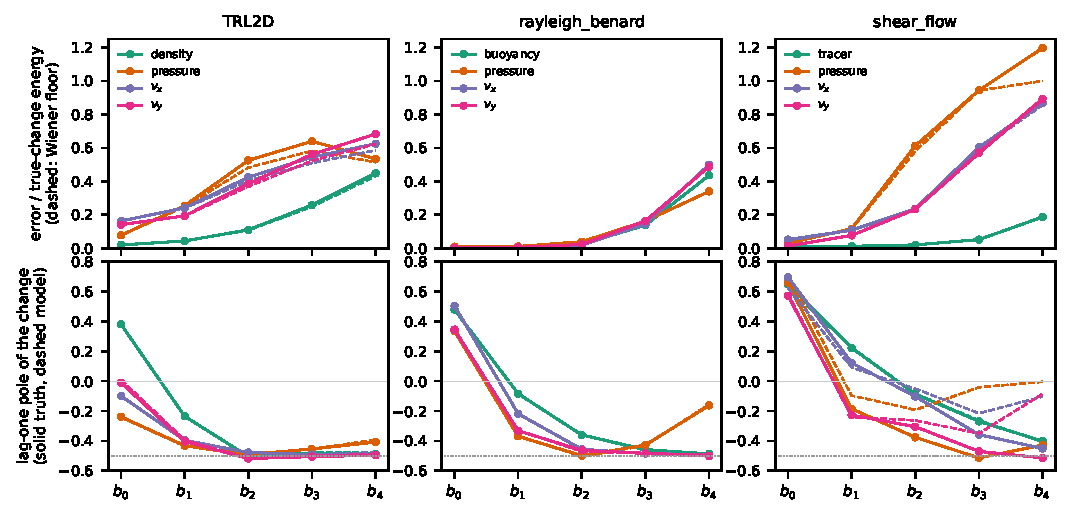
\includegraphics[width=\linewidth]{fig_spectral.pdf}}{}
\caption{What is left after the gate, per Fourier octave $b_0$ (coarsest) to $b_4$. Top: error energy over the octave's
true-change energy (solid) and its Wiener floor, $1-$coherence (dashed). Bottom: lag-one regression slope of the octave's next change on the last observed change (teacher-forced),
truth (solid) against the final model (dashed); the dotted line marks $-\tfrac12$, the value frame-to-frame white content
gives. TRL2D: full test split; rayleigh\_benard and shear\_flow: stratified test samples.}
\label{fig:spectral}
\end{figure}

\section{Per-seed results for the TRL2D official and sliding-start protocols}
\label{app:perseed}

\begin{figure}[h]
\centering
\IfFileExists{fig_multistart.pdf}{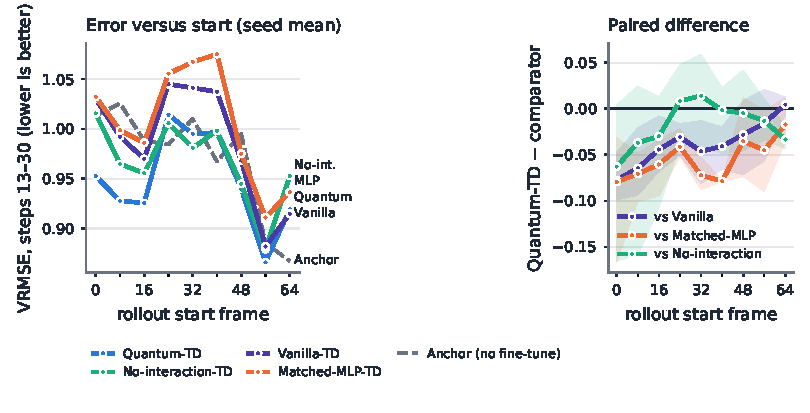
\includegraphics[width=0.66\linewidth]{fig_multistart.pdf}}{\fbox{\parbox{0.9\linewidth}{\centering\pendingnum{fig\_multistart.pdf missing}}}}
\caption{Rollout error versus start frame under the sliding-start protocol. \emph{Left:} seed-mean 13:30 VRMSE per arm
at each start (anchor dashed). \emph{Right:} paired difference, register minus comparator (seed mean, band $=$ seed
range; below zero $=$ register better). The edge over the fine-tuned classical controls persists across starts; the
difference from the anchor is negative only at early starts.}
\label{fig:multistart}
\end{figure}

\begin{table}[h]
\centering
\caption{TRL2D long-horizon window 13:30 test VRMSE (TD fine-tuning, 3 seeds). Right: seeds on which the register
beats that model, by the pre-registered test over start frames (Holm-corrected) and by an uncorrected test over
all 81 trajectory-start pairs. Per-seed values and bootstrap intervals: Appendix~\ref{app:perseed}.}
\label{tab:trl2d}
\small
\setlength{\tabcolsep}{4pt}
\begin{tabular}{lcccc}
\toprule
Model & from the official start frame & mean over 9 start frames & seeds better (Holm) & seeds better (81 pairs) \\
\midrule
$+$ 30-atom register & \TDquantum & \MSquantum & --- & --- \\
$+$ register, $V_{ij}{=}0$ (no interactions) & \TDnoent & \MSnoent & 1/3 & 1/3 \\
released checkpoint (anchor) & 1.0132 & \MSanchor & 0/3 & 1/3 \\
$+$ register, mean-field (Gutzwiller) & \TDgutz & \MSgutz & 0/3 & 0/3 \\
vanilla continued & \TDvanilla & \MSvanilla & \textbf{2/3} & \textbf{3/3} \\
$+$ matched MLP & \TDmlp & \MSmlp & \textbf{2/3} & \textbf{3/3} \\
\bottomrule
\end{tabular}
\end{table}

\paragraph{Four-seed replication.} Registered before any run of seed 1340: one more seed per arm, with the same recipe,
checkpoint selection (best rollout VALID) and evaluation. The effect counts as replicated only if seed 1340's primary test
is significant against both fine-tuned controls, Holm across four seeds. It is not. At seed 1340 all three arms selected
checkpoints from the first 72--84 steps (seeds 1337--1339: steps 5,726--9,309), and the register is the worst of the three:
start-averaged 13:30 VRMSE 0.9568 against 0.8996 (MLP) and 0.8939 (vanilla), worse on all nine trajectories against each.
Over four seeds the register is significant against the MLP on 2/4 seeds and against vanilla on 1/4
(Table~\ref{tab:tdrepl}). The four-seed start-averaged means are 0.9506 (register), 0.9635 (vanilla) and 0.9780
(MLP), and the per-seed tests support no edge. A secondary analysis scores every arm's final step-10{,}000 weights with the same tests. It was
registered after the early selection was seen for the register and before any final-step evaluation, and it cannot
change the primary verdict. There the register is significant against the MLP on 0/4 seeds and against vanilla on 2/4,
so the edge over the MLP seen on three seeds depended on validation-based checkpoint selection.

\begin{table}[h]
\centering
\caption{TRL2D TD replication, four seeds (1337--1340): 13:30 test VRMSE (mean $\pm$ SD over seeds) at the
VALID-selected checkpoints (primary) and at the final training step (secondary), the seeds on which the register is
significantly better (per-trajectory Wilcoxon on start-averaged error, Holm across four seeds), and the seed-1340
official-start value.}
\label{tab:tdrepl}
\small
\IfFileExists{td_repl_table.tex}{\begin{tabular}{llcccc}
\toprule
Checkpoint & arm & official start & all 9 starts & reg.\ better (Holm, 4 seeds) & seed 1340 \\
\midrule
VALID-selected & register & 0.9660 $\pm$ 0.0515 & 0.9506 $\pm$ 0.0193 & --- & 1.0056 \\
 & matched MLP & 1.0101 $\pm$ 0.0490 & 0.9780 $\pm$ 0.0539 & 2/4 & 0.9439 \\
 & vanilla continued & 0.9892 $\pm$ 0.0897 & 0.9635 $\pm$ 0.0491 & 1/4 & 0.8664 \\
\midrule
final step & register & 1.0467 $\pm$ 0.0684 & 1.0242 $\pm$ 0.0203 & --- & 1.1009 \\
 & matched MLP & 1.0109 $\pm$ 0.0507 & 0.9723 $\pm$ 0.0373 & 0/4 & 0.9841 \\
 & vanilla continued & 1.1236 $\pm$ 0.1669 & 1.0877 $\pm$ 0.0978 & 2/4 & 1.1456 \\
\bottomrule
\end{tabular}
}{}
\end{table}

Table~\ref{tab:perseed} lists every TD arm's per-seed official-start (start-0) 13:30 test VRMSE, its all-start value,
and its rollout-validation selection best (VRMSE@8 at the selected checkpoint). Table~\ref{tab:msfull} gives the
pre-specified statistics of the register against each comparator. The sliding-start protocol reproduces the official
protocol exactly at start 0 (checked to machine precision). Its primary test is a per-trajectory paired Wilcoxon on
13:30 VRMSE averaged over the nine starts ($n{=}9$, one-sided, Holm across seeds); the secondary uses per-(trajectory,
start) pairs ($n{=}81$, correlated within trajectory, uncorrected). Per-window $p$-values on the one-step endpoint are
anti-conservative because windows overlap within trajectories and are read together with seed-level consistency.

\begin{table}[h]
\centering
\small
\resizebox{\linewidth}{!}{%
\begin{tabular}{lccc}
\toprule
Arm & 13:30, official start (s1337/s1338/s1339) & 13:30, all starts & selection best \\
\midrule
official checkpoint (anchor) & 1.0132 & \MSanchor & --- \\
vanilla continued & 1.0787 / 1.0216 / 0.9901 & 1.0091 / 0.9784 / 0.9727 & 0.5846 / 0.5909 / 0.5750 \\
$+$ matched MLP & 1.0328 / 1.0060 / 1.0578 & 0.9993 / 1.0221 / 0.9911 & 0.5716 / 0.5796 / 0.5802 \\
$+$ 30q, $V_{ij}{=}0$ & 1.0202 / 0.9701 / 1.0564 & 0.9437 / 0.9602 / 0.9954 & 0.5923 / 0.5807 / 0.5739 \\
$+$ 30q, mean-field & 1.1882 / 0.9592 / 1.0011 & 1.0222 / 0.9732 / 0.9390 & 0.5847 / 0.5870 / 0.5838 \\
$+$ 30q Rydberg & 0.9927 / 0.9745 / 0.8911 & 0.9620 / 0.9618 / 0.9219 & 0.5783 / 0.5771 / 0.5642 \\
\bottomrule
\end{tabular}}
\caption{Per-seed values behind Table~\ref{tab:trl2d}. The mean-field arms' official-start 6:12 values are
0.5029/0.5221/0.5397; all arms' 6:12 means are 0.5216--0.5278 (anchor 0.5482).}
\label{tab:perseed}
\end{table}

\begin{table}[h]
\centering
\footnotesize
\setlength{\tabcolsep}{3.5pt}
\resizebox{\linewidth}{!}{%
\begin{tabular}{llrcccccc}
\toprule
comparator & seed & mean diff & prim.\ win & prim.\ $p$ & Holm & sec.\ win & sec.\ $p$ & bootstrap CI$_{95}$ \\
\midrule
vanilla & 1337 & $-0.0471$ & 0.78 & 0.0195 & 0.0391$^*$ & 0.59 & $5.0{\times}10^{-3}$ & $[-0.0833, -0.0129]$ \\
vanilla & 1338 & $-0.0167$ & 0.78 & 0.1016 & 0.1016 & 0.57 & $2.3{\times}10^{-2}$ & $[-0.0393, +0.0101]$ \\
vanilla & 1339 & $-0.0508$ & 0.89 & 0.0039 & 0.0117$^*$ & 0.77 & $7.5{\times}10^{-8}$ & $[-0.0702, -0.0260]$ \\
\midrule
matched MLP & 1337 & $-0.0372$ & 0.78 & 0.1016 & 0.1016 & 0.53 & $1.9{\times}10^{-2}$ & $[-0.0795, +0.0079]$ \\
matched MLP & 1338 & $-0.0603$ & 1.00 & 0.0020 & 0.0059$^*$ & 0.75 & $5.2{\times}10^{-8}$ & $[-0.0889, -0.0339]$ \\
matched MLP & 1339 & $-0.0692$ & 1.00 & 0.0020 & 0.0059$^*$ & 0.77 & $1.0{\times}10^{-8}$ & $[-0.0929, -0.0462]$ \\
\midrule
anchor & 1337 & $-0.0086$ & 0.56 & 0.5449 & 1.0000 & 0.44 & $4.9{\times}10^{-1}$ & $[-0.0981, +0.0725]$ \\
anchor & 1338 & $-0.0089$ & 0.44 & 0.6328 & 1.0000 & 0.48 & $5.0{\times}10^{-1}$ & $[-0.0900, +0.0571]$ \\
anchor & 1339 & $-0.0488$ & 0.56 & 0.1504 & 0.4512 & 0.56 & $3.5{\times}10^{-2}$ & $[-0.1206, +0.0249]$ \\
\midrule
$V_{ij}{=}0$ & 1337 & $+0.0183$ & 0.11 & 0.9512 & 1.0000 & 0.30 & $1.0$ & $[-0.0706, +0.0737]$ \\
$V_{ij}{=}0$ & 1338 & $+0.0016$ & 0.44 & 0.5000 & 1.0000 & 0.54 & $4.6{\times}10^{-1}$ & $[-0.0333, +0.0391]$ \\
$V_{ij}{=}0$ & 1339 & $-0.0735$ & 0.89 & 0.0039 & 0.0117$^*$ & 0.67 & $9.5{\times}10^{-5}$ & $[-0.1152, -0.0350]$ \\
\midrule
mean-field & 1337 & $-0.0602$ & 0.44 & 0.4102 & 0.5703 & 0.40 & $5.4{\times}10^{-1}$ & $[-0.2393, +0.0877]$ \\
mean-field & 1338 & $-0.0115$ & 0.44 & 0.2852 & 0.5703 & 0.53 & $2.0{\times}10^{-1}$ & $[-0.0349, +0.0090]$ \\
mean-field & 1339 & $-0.0172$ & 0.56 & 0.1504 & 0.4512 & 0.51 & $1.2{\times}10^{-1}$ & $[-0.0447, +0.0101]$ \\
\bottomrule
\end{tabular}}
\caption{Sliding-start protocol: register minus comparator on start-averaged 13:30 VRMSE, per seed. $^*$: Holm-adjusted
$p < 0.05$. CI: trajectory cluster bootstrap (10{,}000 resamples) of the mean paired difference.}
\label{tab:msfull}
\end{table}



\begin{figure}[h]
\centering
\IfFileExists{fig_training.pdf}{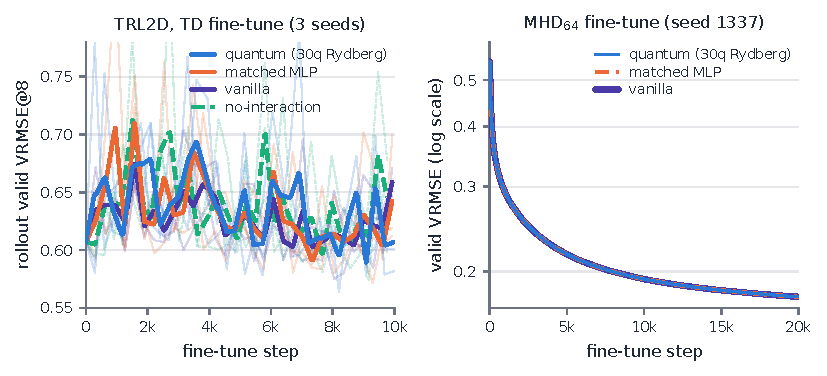
\includegraphics[width=0.52\linewidth]{fig_training.pdf}}{}
\caption{Fine-tuning dynamics. \emph{Left:} TRL2D TD fine-tuning from the official checkpoint (thin: seeds; bold:
3-seed mean of the rollout-validation selection metric); arms overlap step by step, and the test-rollout separation
is not visible in validation curves. \emph{Right:} \texttt{MHD\_64} (seed 1337, log scale); all arms converge to
per-channel validation VRMSE $\approx$0.177.}
\label{fig:training}
\end{figure}

\section{Qubit-ladder details}
\label{app:ladder}



Per-seed VRMSE@8 (s1337/s1338/s1339) under TD: 5 atoms 0.9245/0.8053/0.7982; 10 atoms 1.1810/0.7799/0.8387; 20 atoms
1.2486/0.7843/0.7478; 30 atoms 0.903/0.826/0.806; matched MLP 1.098/0.933/0.829; mean-field pilot 0.891/0.825/0.802.
Seed 1337 is the outlier at every interior count. Under the one-step arena objective the means were 30 atoms
$1.1002 \pm 0.1939$, matched MLP $1.0574 \pm 0.0574$ and bare backbone $0.9637 \pm 0.0048$: the adapters' edge appears only
under TD. A smoke-scale CMA-ES configuration search (about 200 evaluations per regime) was not competitive with
gradient training.

\section{MHD\_64}
\label{app:mhd}

The released \texttt{MHD\_64} checkpoint evaluates to 0.5447 (test) / 0.5464 (validation) per-channel VRMSE under our
pipeline ($\approx$0.66 field-grouped, the convention of the published 0.1633); the same pipeline reproduces the TRL2D
anchor to 1.1\%, which points to, but does not prove, a discrepancy in the released artifact. Four of the nine 20k-step
runs stopped at about 7.5k steps; the primary row uses the two seeds at which all three arms reached the same length
(backbone $0.1897 \pm 0.0178$, MLP $0.1897 \pm 0.0178$, register $0.1896 \pm 0.0177$; the arms agree to four decimals and
the gate never opens). All arms beat the released artifact on every one of 960 test windows.

\paragraph{Physics constraints on the classical part (registered).} The true magnetic field is divergence-free on this
periodic grid (longitudinal energy share $8\times10^{-6}$), while 6\% of the backbone's field error is longitudinal, and
the backbone, which zero-pads and down-samples, is not shift-equivariant. Projecting the predicted field onto its
divergence-free part in physical units lowers the gated model's full-test VRMSE from 0.1725 to 0.1709 per channel
(0.1853 to 0.1840 field-grouped); averaging over eight circular shifts of the input as well gives
0.1592$^\dagger$ (0.1707$^\dagger$), lower in every channel and in every octave, with the predicted high-wavenumber
energy shrinking by about 3\%. $^\dagger$Eight-fold test-time averaging, eight times the inference cost; the published
model did not average. On the published convention both remain above 0.1633 and far above the current best, 0.1160
(EddyFormer, \citealp{du2025eddyformer}; Flowers 0.1165). Both steps change the classical part of
every arm equally.

\section{Learned register configurations}
\label{app:registers}

\begin{figure}[h]
\centering
\IfFileExists{fig_config3d.pdf}{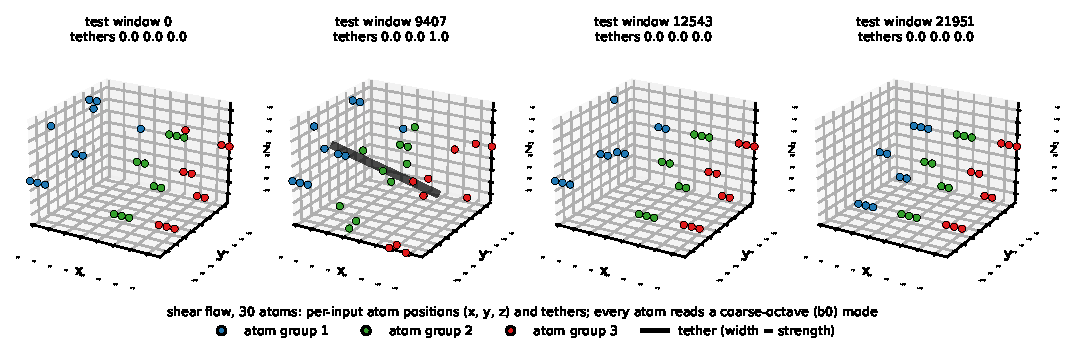
\includegraphics[width=\linewidth]{fig_config3d.pdf}}{}
\caption{Per-input qubit configuration in 3-D (routed register, 3-D variant of Appendix~\ref{app:hscale}, shear flow,
30 atoms, seed 1): atom positions $(x,y,z)$ of the three 10-atom groups (drawn side by side) on four test windows, and
tether strength between groups (line width). Positions move with each input (mean 0.33, at most 1.36 grid units from
the mean layout; $z$ spans 2.1), and on window 9407 the network switches on the tether between groups 1 and 3. The variation is shown, not shown
useful: swapping positions or tethers between inputs changed VALID error by at most 0.21\% (registered, 3 seeds).}
\label{fig:config3d}
\end{figure}

\begin{figure}[h]
\centering
\IfFileExists{fig_registers.pdf}{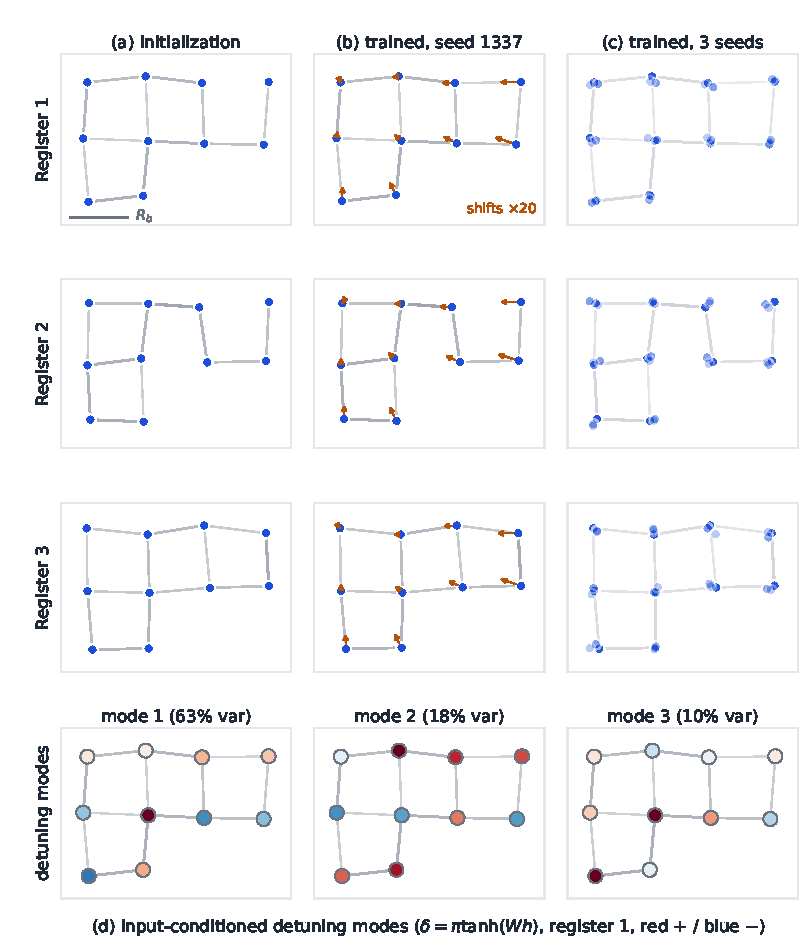
\includegraphics[width=0.5\linewidth]{fig_registers.pdf}}{}
\caption{Register configurations (three blockade-decoupled 10-atom registers, trainable 2-D geometry, blockade-radius
units). \emph{(a)}~Initialization (lattice with $\sigma{=}0.05\,R_b$ jitter). \emph{(b)}~TD-trained geometry (seed
1337, displacements $\times 20$): a small coherent contraction (mean radial shift $-0.007\,R_b$). \emph{(c)}~Three seeds
agree to $\le 0.11\,R_b$ rms. \emph{(d)}~Per-input reconfiguration via detunings: the top three singular modes of the
conditioning map hold 91\% of its variance.}
\label{fig:registers}
\end{figure}

\section{Visual rollout fields: TRL2D and MHD\_64}
\label{app:fields}

\begin{figure}[h]
\centering
\begin{minipage}[t]{0.54\linewidth}
\centering
\IfFileExists{fig_fields.pdf}{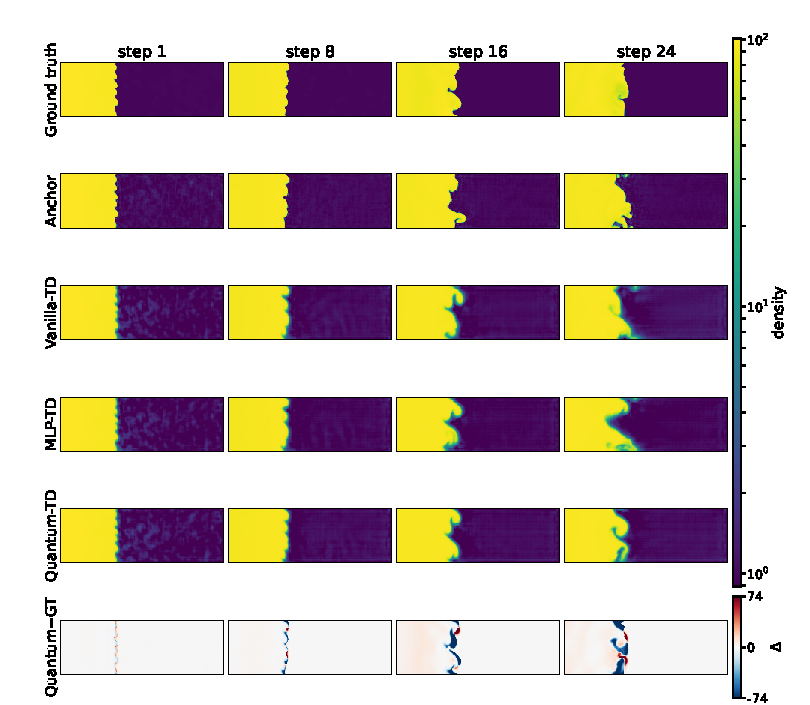
\includegraphics[width=\linewidth]{fig_fields.pdf}}{}
\caption{Ground truth vs model rollouts on the first TRL2D test trajectory (density, log scale; bottom: signed error of
the TD register arm). Error concentrates at the mixing front. On this trajectory the anchor has the lowest late-step
VRMSE (0.640/0.659 at steps 16/24 vs 0.890/0.712 for the register arm); headline claims rest on full-test-set
averages.}
\label{fig:fields}
\end{minipage}\hfill
\begin{minipage}[t]{0.43\linewidth}
\centering
\IfFileExists{fig_fields_mhd.pdf}{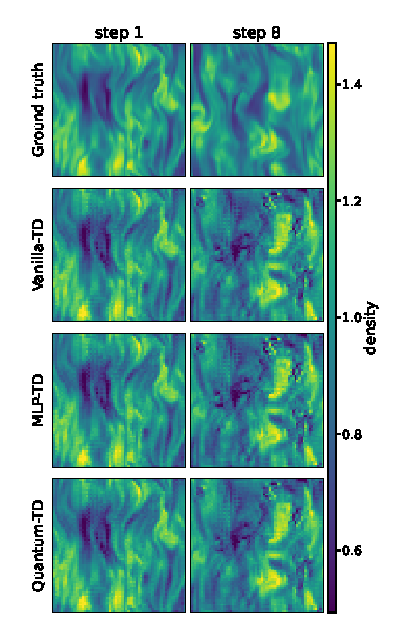
\includegraphics[width=\linewidth]{fig_fields_mhd.pdf}}{}
\caption{Ground truth vs model rollouts for 3D magnetohydrodynamics (MHD\_64, valid trajectory 0, mid-$z$ density slice, steps 1 and 8). Top to bottom: Ground truth, Vanilla-TD, matched MLP-TD, and Quantum-TD. All arms preserve coarse density topology; fine discrepancies concentrate in turbulent magnetic shear interfaces.}
\label{fig:fields_mhd}
\end{minipage}
\end{figure}

\section{Dynamic configuration and hardware mapping}
\label{app:dynamic}

\begin{table}[h]
\centering
\caption{What maps to current neutral-atom devices, from the vendors' public programming interfaces (QuEra Aquila via
Amazon Braket's analog Hamiltonian simulation schema; Pasqal Fresnel and Pulser's detuning map modulator, DMM).}
\label{tab:hardware}
\scriptsize
\setlength{\tabcolsep}{3pt}
\begin{tabular}{p{0.2\linewidth}p{0.25\linewidth}p{0.23\linewidth}p{0.24\linewidth}}
\toprule
 & Our registers & QuEra Aquila & Pasqal Fresnel \\
\midrule
Geometry & 2-D, $3\times10$ atoms; routed co-processor adds per-input 2-D offsets & user-defined 2-D arrangement & 2-D on calibrated trap layouts; $\le$80 atoms, $\ge$5\,\textmu m apart, within 38\,\textmu m \\
Drive & global $\Omega$, $\phi$ per layer & global $\Omega(t)$, $\phi(t)$ & global Rydberg channel \\
Detuning & signed, per atom, per layer, input-dependent & global $\Delta(t)$; local $\Delta_\ell(t)\,h_k$, $h_k\in[0,1]$ static (experimental) & global $\Delta(t)$; DMM: negative only, one waveform, static weights in $[0,1]$ \\
Readout & $\langle Z\rangle$, $\langle X\rangle$, $\langle Y\rangle$ & ground/Rydberg bitstrings & ground/Rydberg bitstrings \\
\bottomrule
\end{tabular}
\end{table}

Table~\ref{tab:hardware} states what a deployment would need. The neck register's 2-D geometry and global drives map
directly, and distances are clamped from below as both devices require. Three features do not map as trained. Signed,
per-layer, input-dependent local detunings would have to be re-encoded as a global detuning plus one static,
one-signed weight pattern per input, which means one device program per input. $\langle X\rangle$ and
$\langle Y\rangle$ readouts need a basis-rotating pulse before measurement. The configuration network also outputs a $z$ offset, but it stays at zero in training (a planar start gives it no gradient), so every learned layout is 2-D.

\paragraph{Finite-shot readout.} A device estimates each atom's $\langle Z\rangle$, $\langle X\rangle$ and
$\langle Y\rangle$ from $N$ shots per measurement setting. We re-evaluated the route-supervised co-processor register
(3 seeds per row, trained exactly as before) with each expectation replaced by $2\,\mathrm{Bin}(N,(1+\langle P\rangle)/2)/N-1$,
drawn independently per atom and axis. This independent-marginal approximation gets each estimate's variance right but
omits the covariance between atoms read in the same shot (a real shot samples a joint bitstring), so it is not a
hardware-fidelity test. Nothing was retrained with noise, and the rule was registered first: under this approximation the register counts as shot-robust at $N$ if the
mean increase in test VRMSE stays below half its gap to the matched MLP. The increase is $7.6\times10^{-5}$,
$8\times10^{-6}$ and $1\times10^{-6}$ on shear\_flow and $3.2\times10^{-4}$, $3.4\times10^{-5}$ and $4\times10^{-6}$ on
rayleigh\_benard at $N=100$, $1{,}000$ and $10{,}000$ (thresholds $5.5\times10^{-5}$ and $1.8\times10^{-4}$). The register is
shot-robust under this approximation from $N=1{,}000$ on both rows and not at $N=100$. Because that gap is itself not significant, we also
compare with seed spread: at $N=1{,}000$ the increase is below the seed standard deviation of every core on
shear\_flow ($1.8$--$3.4\times10^{-4}$) and of the classical cores on rayleigh\_benard ($3.1$--$3.7\times10^{-4}$), though not
below the register's own spread there ($2.2\times10^{-5}$). With the three 10-atom groups run in parallel on a 30-atom
array, the measured cost per input is $3N$ shots (three settings) when the tethers are inactive, as in five of the six
shot-study fits (their tethers are fixed, not set per input); the single nonzero tether (shear\_flow seed 1, group 0 to
group 2) needs two rounds, $6N$, and a full three-group chain would need up to $9N$. A 10-atom device reused in turn needs
$9N$ group executions. The matched classical cores need none of this.
Calibration errors were tested the same way (registered first; 3 seeds, 3 repeats): Gaussian in-plane position jitter
of 1\% and 5\% of the lattice spacing and a multiplicative detuning error of 1\% and 5\% per atom and layer. Jitter and
the 1\% detuning error raise test VRMSE by at most $7\times10^{-6}$ on both rows; a 5\% detuning error costs
$1.4\times10^{-4}$ on rayleigh\_benard (within its threshold) and $7.3\times10^{-5}$ on shear\_flow (above its
$5.5\times10^{-5}$ threshold). The register tolerates placement errors well and needs detunings calibrated to about 1\%.


Detunings depend on each input; geometry, drives and evolution times are shared learned parameters in the reported
arms, and each forward pass resets the register. An arena-only variant with input-conditioned positions
$r_i(h) = r_i^0 + 0.6\tanh(g_\phi(h)_i)$ reached \QLgeo, worse than the static layout. Mapping to a neutral-atom device
would require: replacing signed per-layer local detunings with the platform's addressable detuning patterns; enforcing
minimum atom separation (clamping regularizes interaction energies but does not enforce physical spacing); replacing the
first-order digital--analog split by continuous pulses; and a noise model beyond finite-shot readout. Optical tweezers
assemble user-defined 2-D arrangements at the 100-atom scale \citep{barredo2018synthetic}, with coherent arrays reported
at 6{,}100 atoms \citep{manetsch2025tweezer}; the registers here use at most 30 atoms in blocks of 10. The trained neck
registers of the audit are inference-inert, so those deployed models need none of this; the routed co-processor is not,
and its readout cost is given above.

\section{Hybrid scaling with the qubit budget}
\label{app:hscale}

Table~\ref{tab:audit}'s convection row was first scored on a stratified test sample (5{,}600 of 34{,}300 windows), the sample this scaling study uses: classical 0.0449, $+$MLP 0.0428, $+$30/50/100 qubits 0.0426/0.0422/0.0412. A registered retraining with the same recipe, scored once on every test window, gives the values now in the table (0.0456, 0.0435, 0.0430/0.0425/0.0418; vs MLP $+1.1\%$ instead of $+0.5\%$, vs classical $+5.6\%$ instead of $+5.1\%$). It is a representativeness check on test data already used, not an independent confirmation.

Registered before the sweep (a 5-qubit smoke run only tested the code). $K$ counts allocated atom slots across groups of
at most 10 atoms: the largest joint quantum state has 10 atoms, and tethers pass classical readouts between groups, so
200 qubits means 20 separately simulated 10-atom groups, not a 200-qubit entangled state. The backbone and cached inputs are fixed; the gate, a classical head for unselected modes and a classical bypass beside
the core on selected modes are retrained with the core at each budget and seed, so budgets compare separately fitted hybrids. The routed co-processor sets every register degree of freedom it can per input: atom
positions ($x,y,z$), detunings, which modes the atoms receive, and, new here, the strength of each tether between the
10-atom groups (a learned base plus a linear map of the routed modes' features). Drives and evolution times stay
shared. Budgets $K\in\{0,5,10,20,30\}$ ($K=0$: classical part alone); register and a similarly sized MLP (199 trainable core parameters against the register's 241, 244 in total); three seeds on
every row (full test on shear\_flow, TRL2D and MHD\_64, stratified test on rayleigh\_benard). The backbone in the classical
part is the vanilla CNextU-net, never trained with a register. A first version of this sweep used, on three rows, a backbone
trained with a register in its neck; it is kept below as a check of how much the backbone matters.

Figure~\ref{fig:hscale} (top) gives the hybrid's test VRMSE relative to its classical part. It falls with the budget
on the two rows with predictable error: to 0.877 (register) and 0.900 (MLP) at 30 qubits on shear\_flow, and to 0.949
and 0.954 on rayleigh\_benard. It stays at 1.000 on TRL2D and MHD\_64. Figure~\ref{fig:fill} shows where the added qubits work. The bottom row of Figure~\ref{fig:hscale} explains the shape in error-energy space,
where orthonormal modes add. The coverage $U(K)$, the best $K$ modes' share of the error energy, is
measured, like the captured share, relative to the error energy of the cached pre-gate anchor, not of the learned
gate's residual, and is computed from the test data for any $K$ (no fitting); each run's own coverage bounds what its $K$ qubits can capture, while
the plotted curve pools runs and is descriptive. It follows the closed form
$U_\infty[1-(1+K/K_0)^{1-a}]$ within 0.015 on every row (0.008 or less except on TRL2D; $U_\infty$ 0.430, 0.0475, 0.555, 0.019 and $a$ 1.92, 2.11, 1.85,
2.62 for shear\_flow, rayleigh\_benard, TRL2D, MHD\_64), a power-law decay of mode energies. $U(K)$ saturates near 200
qubits because the band-wise POD basis spans only that share of the anchor's error energy: the limit beyond it is the basis, not the
qubit count, and a richer or input-adaptive basis (wavelet packets, a best basis per input) is what would raise it.
The qubits reach $\eta(K)=$ mean captured$/$mean $U(K)$ of the coverage, where $U(K)$ is the curve pooled over both
cores, all budgets and seeds (each arm's gate is trained separately, so a run's own coverage differs; against the
register runs' own coverage $\eta$ is 0.78 and 0.81 on shear\_flow and 0.81 and 0.83 on rayleigh\_benard at 100 and 200
qubits), rising from 0.34 to 0.63 on shear\_flow and from 0.42 to
0.65 on rayleigh\_benard between 5 and 30 qubits; on TRL2D $U_\infty$ is large but $\eta$ is effectively zero, the residual no tested corrector
captured (Appendix~\ref{app:gate}). At 30 qubits the register captures 54\% of what the basis allows on shear\_flow (86\% at its
current efficiency); the shaded fans extrapolate beyond 30 qubits with $\eta$ held at its 30-qubit value or at 1.
The fan was tested at 50 qubits (five groups, same per-input layout), with ranges for the register's capture
registered before any run: $[0.249, 0.380]$ on shear\_flow and $[0.027, 0.040]$ on rayleigh\_benard. The upper edges
come from the pooled coverage (only a run's own coverage is a strict bound on its capture), so the test is whether $\eta$ falls below its 30-qubit value. All six
seeds fell inside (shear\_flow 0.255, 0.253, 0.269; rayleigh\_benard 0.029, 0.028, 0.028), near the lower edges, with
$\eta$ rising slightly (0.63 to 0.66 and 0.65 to 0.70), and the hybrid reached 0.869 and 0.940 of its classical part. The matched MLP did as well or better (shear\_flow 0.268, 0.263, 0.302; rayleigh\_benard 0.028, 0.027, 0.028; hybrid
0.877 and 0.940), so at 50 qubits too the gain belongs to the routing, not the register. At 100 qubits a registered
replication on five new seeds (4--8), with the rule fixed before any 200-qubit register result, found the one
exception: on shear flow the register's test VRMSE was below its matched MLP's on 5 of 5 seeds (means 0.0202 against
0.0207, 2.5\%; one-sided paired $t$-test $p=0.0065$, below 0.05 even after a Holm correction over the four registered
cells). This MLP has 199 trainable core parameters against the register's 241 (244 in total; the MLP's hidden width is an
integer), and it
does not see the register's interaction graph; a one-unit wider MLP (297) and a graph-aware GNN of 239 parameters that learns its
own interaction graph with the same geometry architecture, both registered before they ran, were scored on all five shared seeds. The register was lower than the GNN on only 2 of the 5 seeds (means 0.02020 against 0.01990; one-sided paired
$p=0.76$) and lower than the wider MLP on 3 of 5 (0.02020 against 0.02053, $p=0.13$), so it does not meet the rule (lower on
at least 4 of 5 and $p<0.05$) against either: the edge is not established against a graph-aware GNN of similar size or a wider MLP.
The GNN learns its own graph and router and normalises its coupling weights, so this does not attribute the original
edge to the graph. The lower mean VRMSE is not accompanied by a
consistently higher captured-energy share (the register's is lower on 3 of the 5 new seeds); the two measures weight
fields and windows differently, and the co-trained gate and head differ between arms. A metric-aligned 100-qubit control
remains pending; the test windows were seen in
earlier rounds, so this is TEST-informed. On rayleigh\_benard the register is below the smaller MLP on 5 of 5
new seeds (0.0410 against 0.0414, 0.9\%, one-sided paired $p=0.029$), which passes the unadjusted rule; the Holm
correction over the four cells waits for the two 200-qubit cells. Against the same two controls on this row the register
was lower than the GNN on 1 of 5 seeds (0.04104 against 0.04078, $p=0.97$) and than the wider MLP on 3 of 5 (0.04104
against 0.04114, $p=0.15$), so it does not meet the rule against either. A registered interaction-free control
(the same register retrained with interaction time fixed at zero, so each atom evolves alone; 3 seeds, VALID) is within
0.5\% of the register on all 3 seeds on rayleigh\_benard (no measurable contribution from atom--atom interaction in
this recipe) and mixed on shear\_flow ($+1.3$, $+0.2$, $-0.7\%$; neither outcome of the rule). Training on the metric itself (mean VRMSE),
promoted on VALID by a registered rule and then scored once on TEST from frozen checkpoints (TEST-informed, two seeds),
lowered TEST error for the register (shear\_flow 0.0195 and 0.0199 from 0.0205 and 0.0208; rayleigh\_benard 0.0418
and 0.0417 from 0.0425 and 0.0427) and by similar amounts for the matched MLP. The metric-aligned loss lowers TEST error for both cores in all four
row-seed pairs, without establishing a register-specific advantage. About 94\% of the capture added
between 30 and 50 qubits lands in the coarsest octave (shear\_flow 0.222 to 0.248 of the error, rayleigh\_benard 0.020
to 0.025); the finer octaves, whose error no tested corrector predicts (Appendix~\ref{app:gate}), barely move.
The same ladder at 50, 100 and 200 qubits on TRL2D and MHD\_64 (registered before any run with the expectation that
$\eta$ stays below 0.15 at every budget; the stated rationale was that their gated residual is not predictable from
the input) leaves the hybrid on its classical part: seed-mean test VRMSE 0.1922 against 0.1922 on TRL2D and 0.1733
against 0.1733 on MHD\_64 at every budget (single seeds differ in the fourth decimal), for the register and the matched
MLP alike (three seeds each). On TRL2D the qubits capture effectively nothing ($\eta\le 2.4{\times}10^{-4}$; at most
$1.2{\times}10^{-4}$ of the error, on one seed). On MHD\_64 the register's capture rises from 0.0015 to 0.0020
of the error (seed means at 50 and 200 qubits; $\eta$ 0.10 to 0.11), inside the registered ranges on all nine seeds,
and the matched MLP captures as much (0.0021 at 200). More qubits did not recover the remaining error with this basis, router and trained correction; whether another
input-conditioned correction could is not tested here.
\begin{figure}[h]
\centering
\IfFileExists{fig_spectral_fill.pdf}{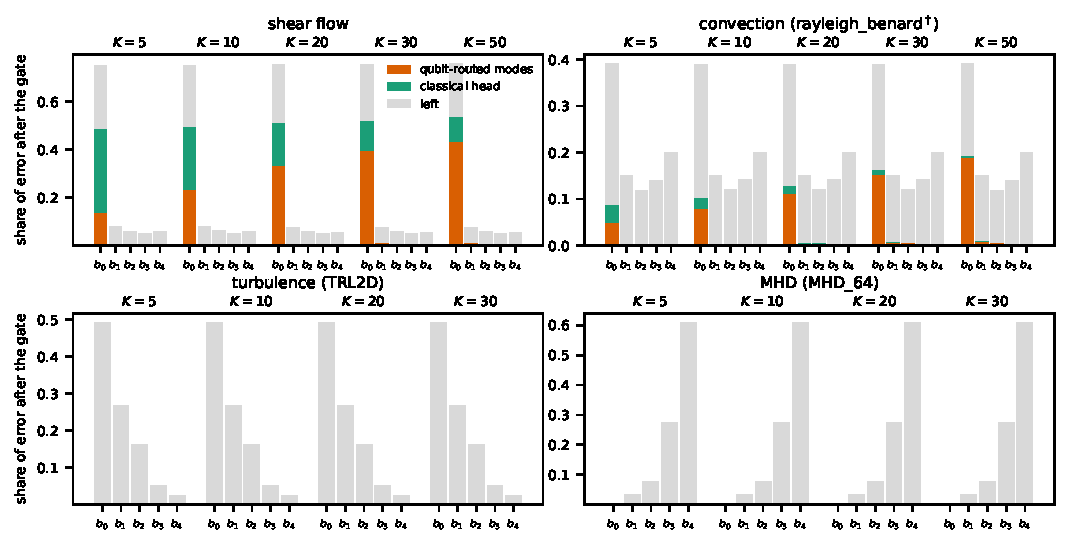
\includegraphics[width=0.92\linewidth]{fig_spectral_fill.pdf}}{}
\caption{Where added qubits work, per Fourier octave ($b_0$ coarsest to $b_4$ finest), register arm, three seeds. Bars (fractions
of the pre-gate anchor's error energy): error after the gate captured by the qubit-routed modes (orange), by the classical head (green), and left (grey). On
shear flow and convection the error sits in the coarse octave and the qubits take it over from the classical head as
$K$ grows; on TRL2D it is spread across octaves and on MHD it sits in the finest octave, and no budget up to 200 qubits captures it here.}
\label{fig:fill}
\end{figure}

\paragraph{100 and 200 qubits (registered).} The same test at 100 and 200 qubits (10 and 20 groups), with ranges
registered before any run from $\eta$ at 50 qubits: $[0.274, 0.405]$ and $[0.279, 0.412]$ on shear\_flow, $[0.0313,
0.0442]$ and $[0.0323, 0.0455]$ on rayleigh\_benard. All twelve seeds fell inside (shear\_flow 0.348--0.354 and
0.369--0.375; rayleigh\_benard 0.037--0.039 and 0.040--0.041), $\eta$ rose to 0.81 and 0.84 at 100 qubits and 0.88
and 0.87 at 200, and the hybrid reached 0.837 and 0.917 of its classical part at 100 qubits and 0.851 and 0.919 at 200.
Past 100 qubits the coverage saturates ($U$ 0.416 at 100 and 0.423 at 200 on shear\_flow), so the extra qubits have
little left to take. The matched MLP reached 0.891 and 0.923 at 100 and 0.859 and 0.917 at 200; the register is below
it on shear\_flow on 3/3 seeds at 100 qubits (paired $p=0.006$) and 2/3 at 200. That comparison was not the registered
test; a registered replication on five new seeds decides it.

\paragraph{Where the gain comes from (registered, 3 seeds).} The position head starts at zero and every atom at $z{=}0$, so the loss has no gradient in $z$ and all trained layouts are 2-D. A control registered before it ran compares, at 30 atoms with the same routing design (each model trained separately), per-input 2-D positions with dynamic tethers (shear\_flow 0.02073, rayleigh\_benard 0.04261), a fixed grid without tethers (0.02071, 0.04258), and a bilayer grid that trains $z$ (0.02110, 0.04271); the matched MLP scores 0.02129 and 0.04281. Neither ``3-D helps'' (1/3 seeds on each row) nor ``geometry and tethers help'' (2/3 and 0/3) passes its rule: no tested geometry or tether variant met the registered gain rule (not an equivalence test). In a validation-only mechanism check registered before its six trainings, swapping positions or tethers across inputs, or replacing positions with the fixed grid, changed the register's VRMSE by at most 0.21\% in any seed; none met the prespecified criterion of a $\geq 0.5\%$ degradation on at least two of three seeds per row. Removing the fitted core term at inference raised VRMSE by 4.8--17.4\% on shear\_flow and 14.2--19.8\% on rayleigh\_benard. Thus the fitted core term contributes at these checkpoints, while the tested per-input configuration perturbations have not shown a material effect under the registered rule. \begin{figure}[t]
\centering
\IfFileExists{fig_outputs_all.pdf}{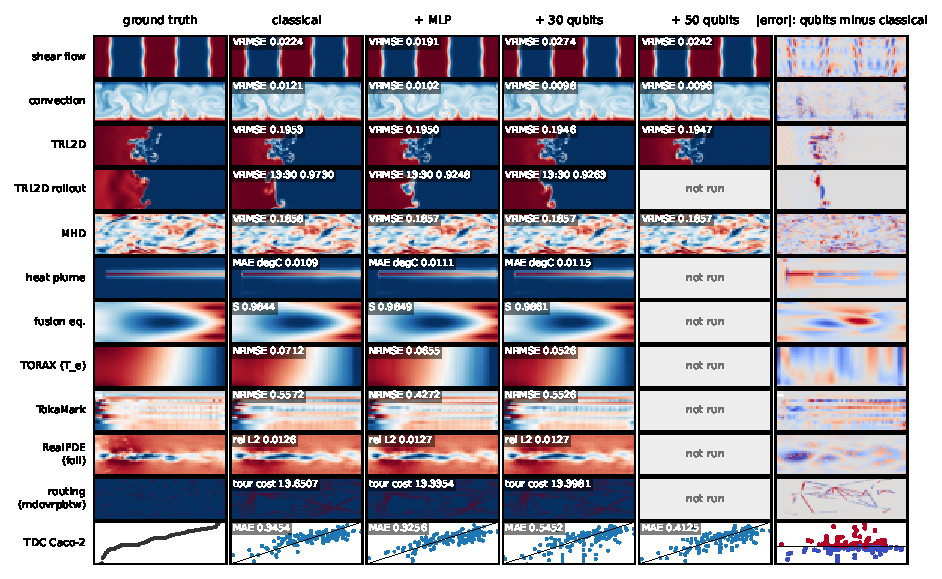
\includegraphics[width=\linewidth]{fig_outputs_all.pdf}}{}
\caption{Figure~\ref{fig:fields_well} at full size, with notes per row (The Well rows show the first output channel; their printed
VRMSE scores all channels of the sample); last column: change in absolute error from classical to qubits (blue: qubits better).
Heat plume: the three predictions agree; the qubits' extra error (MAE 0.0115 against 0.0109\,$^\circ$C) sits on the
steepest tenth of the plume (91\% of the net excess), and elsewhere the net error change is small. Fusion equilibrium (PCA backbone, held-out TEST; panels give the
split's mean official score $S$): classical 0.9844, MLP 0.9849, qubits 0.9861; the flux maps agree to $R^2$ 0.9993, and
the qubits' gain is in the shape of the flux surfaces, not visible at this scale. TORAX (vertical axis: time along a 32-step rollout; horizontal: normalized radius): on this sample (seed 1337) the
clearest gain (0.0526 against 0.0712; MLP 0.0655), growing with lead time and largest at the magnetic axis; over three
seeds the register and its MLP are close (VRMSE@8 0.0305 against 0.0309, classical 0.0321; register ahead on 1 of 3). RealPDEBench: the MLP and
register corrections differ by less than 1\% of the field's spread and leave the U-Net's wake unchanged. TRL2D rollout (VALID-selected rollout
checkpoints, seed 1337; official start; the trajectory with the median classical error; density at step 22 of 30): on
this trajectory the MLP and the register stay closer to the truth than the classical model (13:30 VRMSE 0.925, 0.926 and
0.973); over the nine test trajectories at this seed the register is lowest (0.993 against 1.033 MLP and 1.079
classical), an edge that does not replicate over four seeds (Table~\ref{tab:tdrepl}). Shear flow, convection and TRL2D
(routed co-processor of Table~\ref{tab:audit}, top, seed 1337; window fixed in advance): on the shear sample the MLP is
lowest (VRMSE 0.0191; 0.0274 at 30 qubits, 0.0242 at 50, classical 0.0224), although over the test split 30 qubits tie
the MLP (0.0213) and 50 qubits are lower (0.0210; classical 0.0237); on convection the sample follows the split (0.0096
at 50 qubits, 0.0098 at 30, 0.0102 MLP, 0.0121 classical; test 0.0425, 0.0433, 0.0435, 0.0458). On TRL2D (window 436) the arms differ only along the front (0.1946 at 30 qubits, 0.1947 at 50,
0.1950 MLP, 0.1953 classical; test 0.1921--0.1923). Routing (RouteFinder, first test instance of the first unseen multi-depot variant, MD-OVRPBTW; no
reference tour is released, so the first column shows depots and customers, and the last column only marks where the
register's and the classical tours differ, not an error): on this instance the MLP's tour is cheapest (13.34 against
13.40 for the register and 13.65 classical); in this 3-D run the register's mean gap over the 16 variants is lowest (8.62\%
against 8.69\% classical and 8.77\% MLP at seed 1; over three seeds 8.67\% against 8.68\% MLP and 8.63\% classical), while at the EAL budget of
Table~\ref{tab:rf} no routed arm beats vanilla (Appendix~\ref{app:routing}). TokaMark (FT-Base recipe; the middle test shot by id, chosen mechanically after the scores were known, 467
windows left to right; rows: the 15 EFIT signals, two for each X-point; blank: no EFIT value): on this shot the MLP is
lowest (NRMSE 0.43 against 0.55 register and 0.56 classical); over all 1{,}020 test shots the task score is 0.1500 MLP, 0.1504
classical and 0.1512 register (one seed, descriptive; our best, 0.1379, uses the Scratch recipe). MHD (routed, test window 480, mid-plane slice): the four arms
agree to 0.0001 (VRMSE 0.1857--0.1858; test 0.1733 each), so the gate carries the whole gain.}
\label{fig:outputs_all}
\end{figure}

\paragraph{3-D, tethered configuration on every benchmark (registered).} A 3-D register (three 10-atom
groups; per-input positions $(x,y,z)$ on a randomly offset 3-D lattice so every coordinate trains; per-input detunings;
per-input tethers that pass each group's readout to the next) replaced the neck register on every benchmark, each against
its own similarly sized MLP. It improves on the classical model on the heat plume (MAE 0.0341 against 0.0364) and TORAX
(VRMSE@8 0.0305 against 0.0321), but its matched MLP gains as much (0.0340, 0.0309); on RealPDEBench every corrector scores
0.00939; on fusion equilibrium it ties its MLP with the starter U-Net ($S$ 0.786 against 0.791), and on the stronger
PCA backbone (held-out $S$ 0.9844) it beats its MLP on 3/3 seeds (0.9861 against 0.9849; paired $p=0.039$ one-sided,
0.078 two-sided), all of it in the $\psi$-derived shape scalars (elongation $R^2$ 0.900 against 0.892); on the FNO arena it beats its MLP on 3/3 seeds
(0.969 against 1.023, $p{=}0.010$), which does not survive correction across benchmarks. A registered screen of seven
configuration levers in the routed co-processor (3-D random lattice, wider per-input shifts, active tethers, depth,
configuration width, their combination, a neighbour-correlator readout) found none that lowers validation error on both
rows. Figure~\ref{fig:outputs_all} shows where the three models differ on one sample per benchmark.

With the register-trained backbone the curves have the same shape: 0.858 (register) and 0.885 (MLP) at 30 qubits on
shear\_flow, 0.961 and 0.957 on rayleigh\_benard, flat on TRL2D.

Exploratory, not the registered test: the register is below its matched MLP in 10 of 12 seed-by-budget cells on
shear\_flow (mean 1.8\%; at 30 qubits 2 of 3 seeds, paired $p=0.30$) and in 11 of 12 on rayleigh\_benard (mean 0.5\%;
3 of 3 at 30 qubits, $p=0.19$); TRL2D and MHD\_64 tie. With fixed tether strengths at 30 qubits the two tied
(Appendix~\ref{app:gate}). The registered rule requires a GNN arm and a majority of rows, so no quantum claim follows.





\section{A distribution of configurations per input}
\label{app:fgn}
On TRL2D the qubits capture no predictable error at any budget ($\eta=0$, Appendix~\ref{app:hscale}), and the change
that the backbone misses behaves like frame-to-frame noise (Appendix~\ref{app:gate}). A single configuration per input can
only predict the mean of that noise. WeatherNext~3 \citep{rasp2026weathernext3} builds its ensembles on functional
generative networks \citep{alet2025fgn}: each member is drawn by feeding one low-dimensional noise vector into the
network's conditional normalization layers, and training minimizes the fair CRPS over two members. We move the noise
into the qubit configuration.

\paragraph{Method.} For each window and ensemble member, a code $\xi\sim\mathcal N(0, I_{32})$ enters only the
input-dependent configuration of Appendix~\ref{app:hscale} (30 qubits, band gate, supervised router, per-input
tethers). It enters in three places:
\begin{itemize}
  \item a feature-wise affine map (scale and shift) of the features that enter the core, the analogue of conditional normalization;
  \item the hidden layer of the network that sets each atom's $x$, $y$, $z$ offset;
  \item the per-input tether logits.
\end{itemize}
Each input therefore gets a distribution over atom positions, detunings and tether strengths, and each draw is one
ensemble member. The three maps start at zero, so training starts at the deterministic hybrid. The gate, the classical
head and the routing stay deterministic, so any spread comes through the co-processor alone.

\paragraph{Loss.} We minimize the fair energy score over two members \citep{gneiting2007scoring}. Dividing by the
target's own spatial variance $D(y)$, as below, weights each window by $1/\sqrt{D(y)}$, so the score is observation-weighted
and not strictly proper (it is minimized by a tilted law); the registered re-run replaces $D(y)$ with a fixed
training-set scale, which keeps it proper. In the orthonormal band-wise POD basis it is exact and cheap. Per field, a member's
distance to the target is $\sqrt{E_{\text{new},m}/D}$, which is that member's VRMSE. The distance between two members
is $\lVert c_m-c_{m'}\rVert/\sqrt D$. For a point forecast the score equals the VRMSE, so the two share one scale.
Unlike a per-point CRPS, which WeatherNext~3 notes can reward members with wrong spatial covariance, it depends on the
joint distribution of each field, although its sensitivity to errors in that covariance is known to be weak
\citep{pinson2013energy}.

\paragraph{Protocol.} Selection is on the VALID energy score with 8 fixed draws; TEST is scored once with 16 draws.
The matched MLP twin shares every noise path; as in Appendix~\ref{app:hscale}, only the register reads the atom
positions. We report:
\begin{itemize}
  \item the energy score;
  \item the benchmark VRMSE of the ensemble mean;
  \item the spread--skill ratio (with the $(M{+}1)/M$ correction);
  \item the deterministic hybrid's VRMSE at the same seeds, for comparison.
\end{itemize}
The protocol was fixed before any run, though after earlier TEST results on these rows (TEST-informed, Appendix~\ref{app:claims}). Repeat runs of the deterministic hybrid at one seed differ by up to 3\% on the
GPU, so single-seed gaps below that are not read.

\paragraph{Results.} Table~\ref{tab:fgn} gives the vanilla-backbone rows. On every row and core the energy score is
16--20\% below the deterministic hybrid's VRMSE, while the ensemble mean's VRMSE is 1--9\% worse. The benchmark metric
therefore does not improve, and this lower score is variance-normalised (not strictly proper). The registered proper re-run (fixed training-set scale; shear\_flow and rayleigh\_benard, seeds 1--3, TEST once) confirms the ordering on every seed: the proper-trained hybrid scores 0.0062--0.0063 and 0.0225--0.0231, against 0.0079--0.0080 and 0.0277--0.0281 for the deterministic hybrid and 0.0069--0.0070 and 0.0234--0.0237 for a Gaussian dressing tuned on VALID under the same score; the matched MLP core scores the same within noise (0.0062--0.0064; 0.0232--0.0235), so the effect is not register-specific. Below, on the variance-normalised score, a Gaussian dressing beats the drawn configurations on some controls. The spread is calibrated on shear\_flow (spread--skill 1.03--1.07)
and under-dispersed on TRL2D (0.57--0.58), where it can only come through the 30 routed modes.

Much of the gain comes from calibrated spread, and on TRL2D a control without training does better. A stationary
Gaussian dressing of the deterministic hybrid, tuned on VALID, reaches 0.163 (0.175 on the routed modes only). The
registered primary control sizes the noise on each mode by that mode's TRAIN residual relative to the window's input
amplitude (the standard deviation of the last input frame), times one scale chosen on VALID. On TRL2D it reaches 0.147
with either core, below the drawn configurations even when their spread is scaled about the ensemble mean by a
VALID-tuned factor $\tau$ (0.152 register, 0.158 MLP, $\tau=2.5$ on every seed). That $\tau$ overshoots the
spread--skill ratio (1.2--1.5) and still lowers the score, which suggests the drawn spread has the wrong profile across
windows rather than the wrong size. On shear\_flow the order reverses on every seed and core (0.017 and 0.018 drawn,
0.019 dressed), as it does on rayleigh\_benard (0.035 drawn, 0.037 dressed), while on MHD\_64 the dressing wins again
(0.128 against 0.139--0.142). The dressing thus wins on the two rows whose remaining error the qubits cannot capture
($\eta\approx 0$, Appendix~\ref{app:hscale}) and loses on the two where they capture most of what the basis allows, a
pattern over four rows only.
Among drawn configurations the register was below its matched MLP on each of the first three seeds on TRL2D and
shear\_flow (paired $p=0.055$ and $0.069$). An extension to six seeds, registered after seeing those three, decides this
by a two-sided paired $t$ test with Holm correction across the two rows and requires the register lower on at least five
seeds. On shear\_flow it is lower on 6/6 seeds, by 3.4\% (Holm $p=0.044$), which meets the rule (0.0171, against 0.0177
for the MLP, 0.019 dressed and 0.021 deterministic). On TRL2D it is lower on 5/6 seeds by 0.8\% ($p=0.12$), which does not
meet the rule, and the untrained dressing beats both cores there. The matched MLP, however, has 199 trainable parameters
to the register's 244, so a second control, registered before it ran, widened the MLP by one hidden unit (297
parameters). Against it the register is lower on only 4/6 seeds on shear\_flow (2.2\%, $p=0.24$), which fails the same
rule: the shear advantage does not survive a wider MLP, and no core effect is claimed. The two MLP widths differ by no
more than seed noise (3/6, $p=0.48$). On TRL2D, reported without a claim, the register is lower than the wider MLP on 5/6
seeds (1.1\%, $p=0.09$).

\begin{table}[h]
\centering
\caption{Distribution of configurations per input (30 qubits, TEST, mean over seeds). ES / det.: energy score over the
deterministic hybrid's VRMSE, same core and seeds. Last two columns (seeds in brackets): the energy score with the
spread scaled by the VALID-tuned $\tau$, and the window-scaled Gaussian dressing of the deterministic hybrid.}
\label{tab:fgn}
\small
\resizebox{\linewidth}{!}{\IfFileExists{fgn_table.tex}{\begin{tabular}{llcccccccc}
\toprule
Row & core & seeds & deterministic VRMSE & energy score & ES / det. & ensemble-mean VRMSE & spread--skill & ES, tuned $\tau$ & dressed (e) \\
\midrule
TRL2D & register & 3 & 0.1922 & 0.1593 & 0.829 & 0.1941 & 0.58 & 0.1517 (3) & 0.1469 (3) \\
 & MLP & 3 & 0.1922 & 0.1612 & 0.839 & 0.1944 & 0.57 & 0.1578 (3) & 0.1470 (3) \\
& \multicolumn{9}{l}{\footnotesize register vs MLP on the energy score: +1.2\% (3/3 seeds, paired $p=0.06$); tuned $\tau$: +3.9\% (3/3, $p=0.08$)} \\
shear\_flow & register & 3 & 0.0207 & 0.0170 & 0.822 & 0.0226 & 1.03 & 0.0171 (3) & 0.0189 (3) \\
 & MLP & 3 & 0.0213 & 0.0179 & 0.839 & 0.0231 & 1.07 & 0.0179 (3) & 0.0190 (3) \\
& \multicolumn{9}{l}{\footnotesize register vs MLP on the energy score: +4.6\% (3/3 seeds, paired $p=0.07$); tuned $\tau$: +4.5\% (3/3, $p=0.14$)} \\
rayleigh\_benard$^\dagger$ & register & 3 & 0.0426 & 0.0352 & 0.827 & 0.0444 & 0.77 & 0.0350 (3) & 0.0368 (3) \\
 & MLP & 3 & 0.0428 & 0.0356 & 0.831 & 0.0447 & 0.88 & 0.0358 (3) & 0.0369 (3) \\
& \multicolumn{9}{l}{\footnotesize register vs MLP on the energy score: +1.0\% (2/3 seeds, paired $p=0.36$); tuned $\tau$: +2.3\% (3/3, $p=0.06$)} \\
MHD\_64 & register & 3 & 0.1733 & 0.1419 & 0.818 & 0.1761 & 0.63 & 0.1419 (3) & 0.1280 (3) \\
 & MLP & 3 & 0.1733 & 0.1392 & 0.803 & 0.1769 & 0.79 & 0.1387 (3) & 0.1281 (3) \\
& \multicolumn{9}{l}{\footnotesize register vs MLP on the energy score: -1.9\% (1/3 seeds, paired $p=0.34$); tuned $\tau$: -2.3\% (1/3, $p=0.33$)} \\
\bottomrule
\end{tabular}
}{}}
\end{table}

\section{Vehicle routing: the routed register on RouteFinder}
\label{app:routing}
\paragraph{Row.} RouteFinder \citep{berto2025routefinder} is a pretrained transformer for vehicle routing. Its released
RF-TE checkpoint reproduces on the 16 variants with 100 customers to a mean gap of 3.126\% (published 3.124\%). The row
we use is its efficient-adapter-layer (EAL) fine-tuning to 16 unseen multi-depot variants, with their protocol:
\begin{itemize}
  \item 10 epochs of 10,000 generated instances, batch 128, learning rate $3{\times}10^{-4}$, last epoch kept;
  \item their test files and their gap to reference solutions;
  \item fp32 for every arm of the qubit ladder; the later 3-D tethered triplet (vanilla, register, matched MLP) ran in
    bf16 mixed precision, matched within the triplet but not with the ladder.
\end{itemize}
The fixed classical part ($K=0$) is the pretrained model fine-tuned this way.
A second routing anchor reproduces as well: the released RRNCO checkpoint \citep{son2026rrnco}, which routes on real
road-network distance matrices, scores 72.160, 23.279 and 73.005 on its three asymmetric CVRP test sets (in distribution,
clustered, out of distribution; published 72.145, 23.282 and 73.010). With the released model frozen and only the routed register trained (RRNCO's own
REINFORCE and real-city generator, 10 epochs $\times$ 10k instances, three seeds), the hybrid is worse on all three sets:
3.71, 3.90 and 3.44\% against 3.49, 3.57 and 3.22\% (gaps against the reference costs implied by the published numbers);
after one epoch at a tenth of the rate it sits at parity (3.48, 3.55, 3.20\%), so the loss grows with training. RRNCO's own PyVRP local search applied at test time to the released model's best
decode lowers the gaps to 2.41, 2.61 and 2.07\% (RADAR: 2.61, 2.62, 2.59\%), at about 0.09\,s of CPU per instance; this
is extra test-time compute, not a like-for-like comparison with RADAR's decode-only numbers.

\paragraph{Routed register.} A pooled insertion would see only the mean node embedding (Proposition~\ref{prop:pool}).
The routed register instead acts per instance:
\begin{itemize}
  \item a learned scorer picks $K$ nodes;
  \item their atoms sit at those customers' own coordinates, scaled to lattice units, plus a bounded learned offset in $x$, $y$, $z$;
  \item groups of at most 10 atoms are joined by tethers whose strengths are set per instance;
  \item each atom's readout ($\langle Z\rangle, \langle X\rangle, \langle Y\rangle$) is written back to its own node through a
  zero-initialized map, so training starts at the pretrained model.
\end{itemize}
The MLP control uses the same routing design, tethers and write-back, trained separately; its core ignores the atom
coordinates.

\paragraph{Two fixes before the reported runs.} First, the multi-depot environment can reach a state with no feasible
action. When a remaining customer cannot be served from any depot, each depot deadlock marks the current depot
unavailable until none is left, and sampling then fails. We let such rows visit any unvisited customer. The change acts
only where the original code would stop, so it leaves every other step as it was. Second, every arm trains on the same
generated instances, because instance differences alone moved one pilot arm by 1.6 points.

\paragraph{Results.} Table~\ref{tab:rf} and Figure~\ref{fig:rf} give the qubit ladder at two budgets. At the pilot
budget the register is ahead of vanilla at every budget tried, and ahead of its matched MLP at 5, 10 and 30 qubits but
behind it at 20. At the
EAL budget no routed arm improves on the fine-tuned model alone: vanilla 8.53\%, matched MLP 8.56\% and register
8.59\% at 30 qubits; at 20 qubits both are worse, register 8.87\% and matched MLP 8.71\% (seed 1). The per-variant counts in Table~\ref{tab:rf} are not
independent evidence, because all 16 variants are scored by one trained policy and move together from run to run. The
early lead does not survive full training, and, as on the physics rows, a matched classical core does what the
register does. With the 3-D tethered register at 30 qubits (EAL protocol, common random numbers, bf16 mixed precision, seed 1, 10 epochs), the
register's gap is 8.62\% against 8.77\% for its matched MLP (1{,}715{,}198 and 1{,}715{,}057 parameters) and 8.69\% for
vanilla at seed 1; over seeds 1--3 the register, the MLP and vanilla average 8.67\%, 8.68\% and 8.63\% (vanilla seeds 2--3 run on a second machine whose seed-1 rerun lands within 0.03 points).
Against the published EAL result (8.58\%, the unweighted mean of Table~11 in \citet{berto2025routefinder}), fp32
vanilla runs give 8.53, 8.60 and 8.82\% (seeds 1--3, mean 8.65\%: parity, not a lead); the first was 0.05 points lower and the bf16 runs are 0.04--0.19 points higher; on 2{,}048 generated validation
instances, decoding in fp32 instead of bf16 changes route cost by $+0.001\%$ (CI $\pm0.05\%$), so the difference sits
in training, not decoding.
With the routed register (30 atoms, the design of Table~\ref{tab:audit}, top) over five seeds in bf16, the mean gap is
8.61\% against 8.65\% for vanilla (better on 2 of 5 seeds; Table~\ref{tab:audit}); with the sampling decode below it is
5.96\% against 6.02\% (3 of 5). Neither difference is outside the seed spread (standard deviation of the paired
difference 0.19 points). A registered gate that applies the register only to time-window instances gives 8.73\%.

\paragraph{Extra decode compute (registered, test files, reported apart).} Multi-start sampling (temperature 0.5,
four samples per start, eight augmentations; $4\times$ the protocol's decode) lowers the register's mean gap from 8.62\%
to 6.03\% and the matched MLP's from 8.77\% to 6.14\% (a harness rerun of the protocol decode reproduces every per-variant
gap within 0.008 points). Register minus MLP is $-0.11$ points (95\% CI $-0.13$ to $-0.09$ over test instances, 8 of 16
variants; one trained policy per arm, so the interval does not cover seed variation). These rows use more test-time
compute than the published protocol and are not compared with 8.58\% as like for like. Post hoc, at seed 1 the register was ahead on all eight time-window
variants and behind on the other eight; a registered test on seeds 2 and 3 did not replicate this (register minus MLP:
$-0.15$, $+0.13$, $0.00$ points at seeds 1--3).

\paragraph{Blockade move selection (registered screen, VALID only).} After the fine-tuned policy builds a route, ten
rounds of local search take the 18 best improving 2-opt and relocate moves, keep a set that do not conflict, and apply
them together. An ideal blockade array (adiabatic sweep, 100 shots) picks that set as a maximum-weight independent set;
exact enumeration is the ceiling. On 128 VALID instances of four unseen variants and two seeds, applying compatible
moves together lowers the mean gap from 14.55\% (policy alone) to 8.39\% (exact), against 9.43\% for one move per round.
On average the array was level with exact (8.38\% against 8.39\%, descriptive; no cell significant after Holm
correction), but greedy selection was only 0.014 points above exact (8.40\%), and from a nearest-neighbour start the
array fell up to 0.15 points behind exact. A control that samples near-optimal sets at random matched the array on 2 of
4 variants, short of the registered 3 of 4 for attributing an edge to random selection; this negative control does not
identify a role for the blockade dynamics either. The registered promotion to TEST
required the array to reach the ceiling in every cell; one policy-start cell missed by 0.026 points, so no TEST run was
made. Exact enumeration of $n\le 18$ moves is instant, so this checks the emulation, not a speed-up. The one robust
result is that, at equal rounds in this fixed pipeline, applying compatible moves together beats one move per round: a
method-level effect, not quantum evidence. At these sizes the choice of selector had little observed effect.

\begin{table}[h]
\centering
\caption{RouteFinder EAL, 16 multi-depot variants: mean test gap to the reference solutions (lower is better). Every arm
trains on the same generated instances. Pilot: 1 epoch of 2,000 instances.}
\label{tab:rf}
\small
\IfFileExists{rf_table.tex}{\begin{tabular}{llccc}
\toprule
Budget & arm & seeds & mean gap (\%) & variants better than vanilla \\
\midrule
pilot & vanilla ($K{=}0$) & 1 & 24.48 & --- \\
 & register, $K{=}5$ & 1 & 23.66 & 14 of 16 \\
 & matched MLP, $K{=}5$ & 1 & 23.80 & 15 of 16 \\
 & register, $K{=}10$ & 1 & 24.31 & 11 of 16 \\
 & matched MLP, $K{=}10$ & 1 & 24.98 & 2 of 16 \\
 & register, $K{=}20$ & 1 & 24.36 & 11 of 16 \\
 & matched MLP, $K{=}20$ & 1 & 23.61 & 14 of 16 \\
 & register, $K{=}30$ & 1 & 23.91 & 13 of 16 \\
 & matched MLP, $K{=}30$ & 1 & 25.05 & 4 of 16 \\
\midrule
EAL protocol & vanilla ($K{=}0$) & 1 & 8.53 & --- \\
 & register, $K{=}20$ & 1 & 8.87 & 0 of 16 \\
 & matched MLP, $K{=}20$ & 1 & 8.71 & 3 of 16 \\
 & register, $K{=}30$ & 1 & 8.59 & 6 of 16 \\
 & matched MLP, $K{=}30$ & 1 & 8.56 & 8 of 16 \\
\bottomrule
\end{tabular}
}{}
\end{table}

\begin{figure}[h]
\centering
\IfFileExists{fig_rf_ladder.pdf}{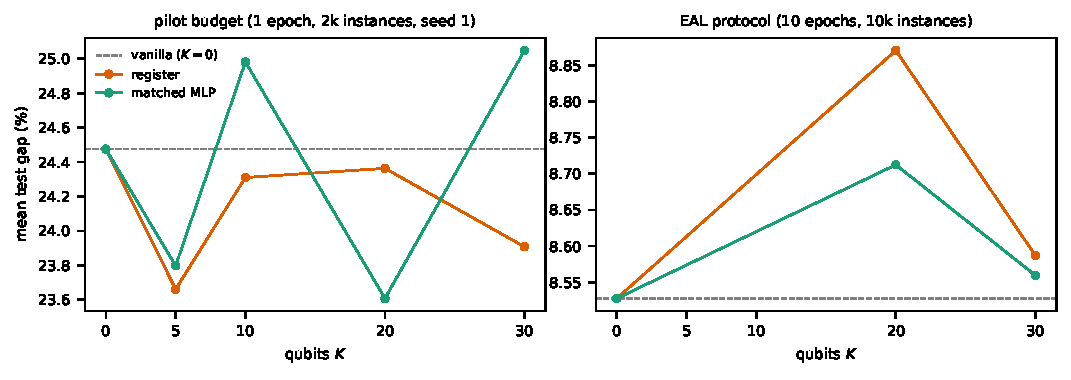
\includegraphics[width=\linewidth]{fig_rf_ladder.pdf}}{}
\caption{RouteFinder qubit ladder with the pretrained model fixed as the classical part ($K=0$, dashed). Left: pilot
budget. Right: EAL protocol. Dots are seeds.}
\label{fig:rf}
\end{figure}

\section{Future work: foundation video world models and long-horizon generative metrics}
\label{app:future_world_models}

While the paper's title and framework refer to \emph{physics world models}, our empirical results in this work
focus on continuous neural PDE surrogates (The Well, RealPDEBench) and physical transport simulators
(TokaMark, TORAX), with one discrete routing row (Appendix~\ref{app:routing}). We explicitly leave the evaluation of open-domain, generative video world models and their
long-horizon benchmarks as future work.

\paragraph{Video world model benchmark suites.} Emerging benchmarks evaluate whether generative video models capture
intuitive physical laws from visual inputs. Specifically, \citet{li2025worldmodelbench} introduce \emph{WorldModelBench},
using visual question-answering judges across physical scenarios, while \citet{punzo2026videophysics} develop
\emph{Physics-IQ} to score video prediction models against counterfactual physical violations. Open-weights video foundation
models such as Wan2.2 \citep{wan2025wan} and LingBot-World \citep{gao2026lingbotworld}, and the 7B world-action model
FLUX 3 Action \citep{flux3action2026}, are multi-billion-parameter diffusion or flow-matching models. FLUX 3 Action decodes
future video frames and robot actions from the same future tokens; that shared latent is where the co-processor would be
inserted, which we have not tested. On our hardware, one Physics-IQ pass costs 13--27 GPU-hours for three arms,
and WorldModelBench needs a VLM judge pipeline on top. We make no empirical claims on video world
model benchmarks in this paper; doing so under matched classical controls is an active direction for future work.

\paragraph{Long-horizon rollouts.} The one candidate regime, rollout-aware fine-tuning evaluated on
long-horizon rollouts (\S\ref{sec:trl2d}), did not replicate at four seeds; more seeds and a checkpoint rule that early
checkpoints cannot dominate are the first requirement. Generative video world models drift away from physically
consistent states over multi-second rollouts. Testing a routed register in the latent bottleneck of such a model, under
the same matched controls, is future work.

\paragraph{Predicting the qubit scaling law.} Appendix~\ref{app:hscale} measures the hybrid's error against the qubit
budget and bounds it by a data-derived coverage curve; how efficiently qubits fill that curve is measured, not
predicted. Recent theory could predict it. For an analog register the accessible frequencies are gaps of its
Hamiltonian's spectrum, so per-input atom positions can give input-conditioned frequency support \citep{wang2026qsm} (in our registered test,
swapping positions between inputs or fixing them to a grid changed VALID error by at most 0.21\%, so this support went
unused; Appendix~\ref{app:hscale});
Fourier-coefficient variance decays with frequency under non-linear embeddings such as our $\tanh$ detunings, a smooth
bias consistent with our probe \citep{kang2026fourier}; pulse-level control changes the optimization landscape more than
the reachable function class \citep{strobl2026pulse}; and finite-shot generalization bounds fix how a readout budget
should be split between inputs and shots \citep{catak2026budget}. Raising the coverage ceiling needs a richer or
input-adaptive mode basis rather than more qubits.

\paragraph{Long-horizon metrics.} One-step scores reward the behaviour we measure in the incoherent bands
(Appendix~\ref{app:gate}): where the prediction's coherence with the true change is low, the least-squares answer shrinks
that band, and over a rollout the shrinkage compounds into lost small-scale energy. Long-horizon evaluation of world
models should therefore report, per Fourier octave and horizon, the prediction-to-truth energy ratio and the coherence,
the lag-one regression slope of each band's change (truth against model), and a proper probabilistic score (CRPS) for ensembles, next
to each benchmark's own rollout metric. We have not run these; they are future work.

\end{document}
